\documentclass[11pt,a4paper]{article}

% Paquets de base
\usepackage[utf8]{inputenc}
\usepackage[T1]{fontenc}
\usepackage{lmodern}
\usepackage{microtype}
\usepackage[shorthands=off,french]{babel}
\usepackage[a4paper,margin=2.2cm]{geometry}
\usepackage{amsmath,amssymb,mathtools}
\usepackage{graphicx}
\graphicspath{{v2/}{../}} % figures v2 (article/v2/figures) en priorité, puis reports/figures
\usepackage{booktabs}
\usepackage{array}
\usepackage{tabularx}
\usepackage{multirow}
\usepackage{makecell}
\usepackage{enumitem}
\usepackage{xcolor}
\usepackage{float}
\usepackage{caption}
\usepackage{subcaption}
\usepackage{longtable}

% Pseudocode
\usepackage{algorithm}
\usepackage{algpseudocode}
\algrenewcommand\algorithmicrequire{\textbf{Entrée :}}
\algrenewcommand\algorithmicensure{\textbf{Sortie :}}

% Références et Liens
\usepackage[hyphens]{url}
\usepackage{hyperref}
\usepackage[nameinlink,capitalise]{cleveref}

\hypersetup{
  colorlinks=true,
  linkcolor=blue!55!black,
  citecolor=blue!55!black,
  urlcolor=blue!65!black,
  pdftitle={Au-delà des heuristiques de dispatching statiques},
  pdfauthor={Jean-Luc MUPASA KALUNGA}
}

% Configuration des légendes et tableaux
\captionsetup{font=small,labelfont=bf} % Légendes petites et labels en gras
\setlist[itemize]{leftmargin=1.5em,itemsep=2pt,topsep=4pt}
\setlist[enumerate]{leftmargin=1.7em,itemsep=2pt,topsep=4pt}
\renewcommand{\arraystretch}{1.15} % Espacement vertical des tableaux

% Suppression du style fancyhdr
\pagestyle{plain} 


% ============================================================================
% MARQUAGE DES RÉVISIONS (version 2, 7 octobre 2026)
% \revmarkstrue  : les passages modifiés apparaissent en bleu, suivis de leur
%                  code entre crochets [M1], [m4]... renvoyant au rapport de
%                  relecture (M = commentaire majeur, m = mineur) ou au
%                  rapport d'audit du code (N = nouveau problème, A = audit).
% \revmarksfalse : version propre, sans couleurs ni balises.
% Les balises orange signalent une expérience encore à faire, les balises
% violettes une décision à valider avec la directrice, les balises vertes
% une figure à régénérer avec les scripts du projet.
% ============================================================================
\newif\ifrevmarks
\revmarkstrue
\definecolor{revcolor}{RGB}{0,70,160}
\newcommand{\revtag}[1]{\ifrevmarks\textsuperscript{\textcolor{red!70!black}{\scriptsize[#1]}}\fi}
\newcommand{\rev}[2]{\ifrevmarks{\color{revcolor}#2}\revtag{#1}\else#2\fi}
\newenvironment{revbloc}[1]{\par\ifrevmarks\color{revcolor}\noindent\revtag{#1}\ \fi}{\par}
\newcommand{\aexp}[1]{\ifrevmarks\textcolor{orange!85!black}{\textbf{[EXPÉRIENCE À FAIRE : #1]}}\fi}
\newcommand{\adir}[1]{\ifrevmarks\textcolor{violet}{\textbf{[À VALIDER AVEC LA DIRECTRICE : #1]}}\fi}
\newcommand{\afig}[1]{\ifrevmarks\textcolor{green!45!black}{\textbf{[FIGURE À RÉGÉNÉRER : #1]}}\fi}

% Macros de rédaction
\newcommand{\pending}[1]{\textcolor{red}{[À COMPLÉTER : #1]}}
% Cadre de figure provisoire (à remplacer par \includegraphics)
\newcommand{\phfig}[2][6cm]{%
  \fbox{\parbox[c][#1][c]{0.92\textwidth}{\centering #2}}}


% Titre et Auteurs
\title{\textbf{Au-delà des heuristiques de dispatching statiques : une évaluation comparative de l'apprentissage par renforcement profond face aux perturbations dans l'exploitation minière à ciel ouvert}}

\author{%
\begin{tabular}{c}
Jean-Luc Mupasa Kalunga$^{1,*}$ \qquad Olfa Ferchichi$^{2}$\\[0.5em]
{\small $^{1}$Faculté d'Informatique, Université Don Bosco de Lubumbashi (UDBL), Lubumbashi, RDC}\\
{\small $^{2}$Laboratoire RIADI, ENSI, Université de la Manouba, Tunis, Tunisie}\\[0.3em]
{\small\texttt{16mk293@esisalama.org; olfaferchichi@yahoo.fr}}\\[0.2em]
{\small \rev{m27}{$^{*}$Auteur correspondant : Jean-Luc Mupasa Kalunga}}
\end{tabular}%
}
\date{} % Pas de date apparente


\begin{document}

\maketitle

\adir{adresse électronique : 16mk293@esisalama.org ne correspond pas à l'affiliation UDBL ; utiliser une adresse institutionnelle UDBL si possible.}

\begin{abstract}
\begin{revbloc}{m1, m2, M1, M3}
Le transport par camions et pelles peut représenter jusqu'à 60\,\% des coûts d'exploitation d'une mine à ciel ouvert et reste très sensible aux perturbations. Les travaux d'apprentissage par renforcement appliqués au dispatching des camions évaluent généralement les politiques dans un seul régime, si bien que leur comportement sous perturbation reste mal connu. Cet article compare huit politiques de dispatching dans un simulateur stochastique : quatre règles heuristiques, deux agents d'apprentissage par renforcement tabulaire, Q-Learning et State--Action--Reward--State--Action, et deux agents d'apprentissage par renforcement profond, Deep Q-Network et Proximal Policy Optimization. Trois régimes sont étudiés : conditions nominales, flotte augmentée de moitié et pannes fréquentes des camions. Chaque combinaison de politique et de régime est évaluée sur 30 réplications appariées, avec des tests non paramétriques corrigés pour les comparaisons multiples. Le classement des politiques change avec le régime : Proximal Policy Optimization obtient la productivité la plus élevée en conditions nominales, l'affectation fixe lorsque la flotte est augmentée et Deep Q-Network lorsque les pannes sont fréquentes, et l'interaction entre politique et régime est significative. Les deux règles fondées sur la seule distance concentrent toute la flotte sur une pelle et sont dominées dans les trois régimes. Évalués sans réentraînement en pannes fréquentes, les agents profonds entraînés en conditions nominales conservent une productivité proche de celle des agents entraînés dans ce régime. Ces résultats suggèrent que la performance nominale prédit mal le comportement sous perturbation et plaident pour une évaluation des politiques de gestion de flotte sur plusieurs régimes contrastés.
\end{revbloc}
\end{abstract}

\noindent\textbf{Mots-clés :} \rev{m1}{Apprentissage par renforcement profond ; Exploitation minière à ciel ouvert ; Dispatching de camions ; Gestion de flotte ; Résilience opérationnelle ; Simulation stochastique ; Proximal policy optimization ; Deep Q-network.}

% ============================================================================
% Section 1 : Introduction
% ============================================================================
\section{Introduction}
\label{sec:intro}

L'exploitation minière à ciel ouvert constitue une pierre angulaire de la chaîne mondiale d'approvisionnement en matières premières, où la viabilité économique des opérations est indissociable de l'efficacité de systèmes logistiques de grande envergure. Il est par conséquent impératif d'explorer les avancées technologiques récentes pour améliorer la performance et la résilience de ces dispositifs logistiques.

% ---------------------------------------------------------
\subsection{Contexte industriel}
% ---------------------------------------------------------

Les mines à ciel ouvert sont des systèmes industriels de très grande échelle dans lesquels le cycle des camions et des pelles constitue l'ossature logistique principale. Ce processus, qui comprend l'excavation, le transport et le déversement des matériaux, n'est pas une simple tâche opérationnelle mais un facteur financier déterminant, représentant jusqu'à 60\,\% des coûts d'exploitation totaux d'un site minier \cite{Afrapoli2017}. Dans l'exploitation minière moderne, la pression pour optimiser ces flux est double : maximiser le débit afin de répondre à la demande mondiale de matières premières, tout en minimisant la consommation d'énergie et les émissions de gaz à effet de serre associées aux flottes de transport diesel.

L'efficacité de ces systèmes est toutefois constamment mise à l'épreuve par une forte variabilité opérationnelle. Dans les environnements miniers réels, les conditions sont loin d'être déterministes. Les pannes d'équipements, les fluctuations de charge utile, les temps de trajet aléatoires causés par la dégradation des pistes et les congestions soudaines du trafic créent ensemble un environnement très instable. La gestion de cette complexité exige une prise de décision en temps réel, capable de concilier la productivité immédiate et la résilience de la flotte.

% ---------------------------------------------------------
\subsection{Notions utilisées}
% ---------------------------------------------------------

\begin{revbloc}{m3, m4}
Cette étude repose sur quelques notions utilisées tout au long de l'article. L'apprentissage par renforcement (Reinforcement Learning, RL) désigne une branche de l'intelligence artificielle dans laquelle un agent autonome apprend un comportement par essais et erreurs, au fil de ses interactions avec un environnement dynamique, de façon à maximiser un signal de récompense cumulée. L'apprentissage par renforcement profond (Deep Reinforcement Learning, DRL) étend le RL en utilisant des réseaux de neurones pour approximer les fonctions de valeur ou les politiques, ce qui permet de traiter des espaces d'états de grande dimension. Le dispatching de camions désigne le processus opérationnel en temps réel consistant à affecter des camions à des points de chargement et de déversement afin d'assurer la synchronisation de la flotte et la productivité ; il est mis en œuvre dans les mines par des systèmes de gestion de flotte (Fleet Management Systems, FMS).

Quatre algorithmes d'apprentissage sont étudiés. Q-Learning et State--Action--Reward--State--Action (SARSA) sont des méthodes tabulaires qui stockent une valeur pour chaque couple état--action. Deep Q-Network (DQN) remplace cette table par un réseau de neurones. Proximal Policy Optimization (PPO) apprend directement une politique au moyen d'une méthode acteur--critique. Les quatre règles de référence sont désignées dans la suite par premier arrivé, premier servi (First-In-First-Out, FIFO), Affectation fixe, Pelle la plus proche et Plus court chemin ; leur définition exacte est donnée dans la \cref{sec:baselines-def}. Enfin, le problème de décision est formulé comme un processus de décision markovien (Markov Decision Process, MDP), plus précisément comme un processus de décision semi-markovien (Semi-Markov Decision Process, SMDP), puisque les décisions sont séparées par des durées variables (\cref{sec:smdp}).
\end{revbloc}

% ---------------------------------------------------------
\subsection{Objectif et organisation de l'article}
% ---------------------------------------------------------

\begin{revbloc}{M23, M24}
L'objectif de ce travail est de déterminer dans quels régimes de fonctionnement une politique de dispatching apprise est préférable à une règle industrielle, et d'expliquer les écarts observés à partir du comportement des politiques. La contribution est évaluative : aucun nouvel algorithme n'est proposé, et l'apport réside dans un protocole de comparaison contrôlé, appliqué à huit politiques et à trois régimes.

Le reste de l'article est organisé comme suit. La \cref{sec:relwork} (\nameref{sec:relwork}) passe en revue la littérature sur le dispatching de camions selon trois paradigmes. La \cref{sec:positioning} (\nameref{sec:positioning}) synthétise cette littérature dans un tableau de positionnement et en déduit la lacune de recherche, le problème étudié, les questions de recherche et les hypothèses. La \cref{sec:contributions} (\nameref{sec:contributions}) présente les contributions et le cadre méthodologique. La \cref{sec:approach} (\nameref{sec:approach}) décrit le système modélisé, le simulateur, la formulation du problème de décision et les agents étudiés. La \cref{sec:design} (\nameref{sec:design}) détaille le protocole expérimental et la \cref{sec:results} (\nameref{sec:results}) les résultats. La \cref{sec:discussion} (\nameref{sec:discussion}) discute ces résultats et leurs limites, et la \cref{sec:conclusion} (\nameref{sec:conclusion}) conclut l'article.
\end{revbloc}

\adir{nouvelle structure de l'article (M24) : à faire valider avant la traduction anglaise.}


\section{Travaux connexes}
\label{sec:relwork}

L'optimisation des systèmes camions--pelles est au c\oe ur de l'ingénierie minière et de la recherche opérationnelle depuis plus de six décennies. \rev{m22}{Comme le soulignent Newman et al.} \cite{AlexandraNewman2010}, l'évolution de ces systèmes est passée de la planification manuelle à des systèmes de gestion de flotte (FMS) automatisés complexes. Cette section passe en revue la littérature autour de trois grands paradigmes : les heuristiques statiques, la programmation mathématique et le domaine émergent de l'apprentissage par renforcement.

\subsection{Dispatching de camions statique et à base de règles}

Le dispatching à base de règles demeure le paradigme dominant dans les mines en exploitation, car il est transparent, peu coûteux en calcul et facile à intégrer dans les logiciels FMS commerciaux. Les premières revues des stratégies de dispatching informatisées \cite{MohanMunirathinam1994} et l'aperçu ultérieur des stratégies de résolution proposé par Alarie et Gamache \cite{Alarie2002} identifient un petit ensemble de règles de décision récurrentes qui structurent encore aujourd'hui la pratique industrielle.

\begin{revbloc}{M25, Dir. corr. 1}
Quatre règles sont particulièrement pertinentes pour la présente étude. La règle premier arrivé, premier servi (FIFO) sert en priorité l'unité de chargement qui attend un camion depuis le plus longtemps ; elle équilibre la charge des pelles mais ignore la configuration spatiale de la fosse. L'Affectation fixe attribue chaque camion à une pelle prédéterminée pour toute la durée du poste ; elle stabilise le facteur d'appariement et reste une référence industrielle répandue, mais ne peut pas réallouer la capacité en réponse à des déséquilibres de files. La Pelle la plus proche envoie le camion vers l'unité de chargement la plus proche, ce qui minimise la distance parcourue à vide au prix d'une optimisation purement locale. Le Plus court chemin généralise cette idée en choisissant la destination qui minimise un coût de cycle estimé sur le graphe des pistes. Les définitions exactes retenues dans cette étude figurent dans le \cref{tab:baselines}.
\end{revbloc}

La performance pratique de ces règles a été évaluée aussi bien sur le terrain qu'en simulation. Subtil et al. \cite{Subtil2011} rapportent une mise en œuvre pratique du dispatching dans une mine à ciel ouvert en exploitation, tandis que Mohtasham et Mirzaei-Nasirabad \cite{MehrnazMohtasham2023} évaluent un progiciel de dispatching commercial dans la mine de cuivre de Sungun et soulignent la sensibilité de la logique à base de règles aux conditions opérationnelles. La simulation à événements discrets a été l'instrument standard de ce type d'évaluation \cite{NecmettinCetin2004, MarceloFioroni2008, Zeng2022, MiladAbolghasemian2020}. Elle montre de façon constante que les règles gloutonnes se dégradent fortement dès que la taille de la flotte dépasse la capacité de chargement de la fosse, car les files d'attente se concentrent sur un sous-ensemble de pelles. \rev{M25, m5}{Les quatre règles retenues ici représentent des logiques différentes : FIFO tient compte de l'état des files, l'Affectation fixe impose une répartition statique et équilibrée, tandis que Pelle la plus proche et Plus court chemin s'appuient sur la proximité spatiale sans tenir compte des files. Les systèmes commerciaux utilisent en outre des règles combinant files et temps de trajet, telles que le temps d'attente minimal des camions \cite{Zeng2022}, ou une couche d'optimisation linéaire en amont \cite{Soumis1989, AmandaSmith2020}, qui ne sont pas incluses dans la présente étude.}

\subsection{Optimisation mathématique et métaheuristiques}

Pour dépasser les limites des règles simples, les chercheurs se sont tournés vers la programmation mathématique. Soumis et al. \cite{Soumis1989} ont proposé une approche à plusieurs étapes combinant la programmation linéaire (PL) pour la planification de la production et des modèles d'affectation pour le dispatching en temps réel. Cette structure modulaire reste l'ossature de nombreux FMS modernes. Ahangaran et al. \cite{Ahangaran2012} ont étendu cette approche en développant des modèles spécifiquement dédiés aux flottes de camions de capacités hétérogènes, en utilisant des réseaux de flots pour équilibrer la production.

Cependant, la nature déterministe de la programmation linéaire en nombres entiers mixtes (MILP) entre souvent en conflit avec la réalité stochastique de l'exploitation minière. Ta et al. \cite{ChungTa2013} ont tenté de combler cet écart en incorporant des probabilités d'inactivité des pelles dans des modèles linéaires, en recourant à la théorie des files d'attente pour obtenir de meilleures estimations de production. Malgré ces avancées, les modèles MILP souffrent fréquemment de la malédiction de la dimensionnalité lorsqu'ils sont appliqués à de grandes mines exploitant des dizaines de camions \cite{AmandaSmith2020, ZhongxinWang2022}.

Pour gérer cette complexité, les métaheuristiques ont été largement appliquées au dispatching et à l'acheminement des camions. Souza et al. \cite{Souza2010} ont démontré qu'une heuristique hybride combinant GRASP et VNS pouvait obtenir des solutions quasi optimales en des temps de calcul réduits. Liu et Chai \cite{GuangweiLiu2019} ont utilisé un algorithme génétique pour minimiser la consommation d'énergie liée au transport tout en tenant compte de la résistance variable des pistes dans le temps. Les algorithmes d'optimisation par colonies de fourmis, qui modélisent la sélection probabiliste d'itinéraires par les insectes sociaux au moyen de mécanismes de mise à jour des phéromones, ont été appliqués aux problèmes d'affectation multi-véhicules dans l'exploitation minière de surface, car leur sélection stochastique s'adapte naturellement aux demandes concurrentes sur des tronçons de piste partagés \cite{ShivPrakashUpadhyay2017}. Le recuit simulé, qui accepte des mouvements sous-optimaux avec une probabilité contrôlée par une température afin d'échapper aux optima locaux, a de même été utilisé pour l'ordonnancement dans les environnements à ciel ouvert \cite{BurakOzdemir2019}. Bien que puissantes, les métaheuristiques sont souvent formulées pour optimiser un état donné du système ou un horizon de planification donné. Lorsque des perturbations importantes modifient les conditions de fonctionnement sous-jacentes, le processus d'optimisation doit être répété ou réoptimisé, ce qui peut limiter la réactivité lorsque les décisions doivent être mises à jour à de courtes échelles de temps dans des environnements miniers dynamiques.

\subsection{Approches par apprentissage par renforcement}

Le passage à l'apprentissage par renforcement représente un changement de paradigme : au lieu de résoudre un nouveau problème d'optimisation à chaque époque de décision, un agent apprend une politique qui associe les états du système à des actions optimales \cite{RichardSutton2018, MoezKrichen2022}. Les premières applications du RL en logistique, comme celles de Nazari et al. \cite{MohammadrezaNazari2018} pour le problème de tournées de véhicules (VRP) et de Zhang et al. \cite{CongZhang2020} pour l'ordonnancement d'atelier, ont démontré que le DRL pouvait surpasser les heuristiques classiques en apprenant à partir de milliers d'interactions simulées.

Au sein de la famille de l'apprentissage par renforcement, les méthodes diffèrent substantiellement par leur puissance de représentation et leur paradigme d'apprentissage. \rev{m5}{Les méthodes tabulaires, telles que Q-Learning et SARSA \cite{RichardSutton2018},} construisent des fonctions de valeur sur des tables d'états-actions discrets, ce qui les rend transparentes et légères en calcul, mais leur expressivité se dégrade fortement lorsque l'espace d'observation croît avec la taille de la flotte. Les agents DQN répondent à ce problème en approximant la fonction Q par un réseau de neurones et en stabilisant l'entraînement grâce au rejeu d'expériences et au gel du réseau cible, ce qui permet de généraliser à des entrées continues de grande dimension. PPO \cite{JohnSchulman2017} appartient à la famille acteur-critique : elle optimise directement la politique via un objectif de substitution dont la contrainte d'écrêtage empêche les mises à jour catastrophiques des paramètres. Ces quatre algorithmes, du tabulaire au profond et de l'approche fondée sur la valeur au gradient de politique, forment un spectre comparatif naturel et constituent précisément la composante RL du banc d'essai conçu dans cette étude.

Dans le secteur minier, cette transition est plus récente. Hazrathosseini et Afrapoli \cite{Hazrathosseini2024} proposent une revue critique, soulignant que, bien que le RL présente un potentiel considérable pour les FMS intelligents, la plupart des études restent au stade de la preuve de concept. de Carvalho et Dimitrakopoulos \cite{deCarvalho2023} ont appliqué un cadre acteur--critique à la planification de la production, montrant que le RL peut traiter efficacement la dynamique de la flotte tout en mettant à jour les objectifs de production.

Des bancs d'essai récents, tels que Mining-Gym \cite{Banerjee2025}, ont commencé à fournir des environnements standardisés pour tester ces algorithmes. Zhao et al. \cite{Zhao2025} ont proposé une approche hiérarchique d'apprentissage par renforcement multi-agent (MARL) pour un dispatching durable, avec un accent sur l'efficacité énergétique, tandis que Pei et al. \cite{Pei2025} et Rosales et Diaz \cite{FranciscoRosales2025} ont exploré le dispatching par apprentissage et le dispatching interprétable pour le transport minier autonome. L'usage d'une aide à la décision fondée sur le RL pour l'ordonnancement industriel hiérarchique dépasse le secteur minier : Szatmari et al.~\cite{KingaSzatmari2025} démontrent des architectures multi-niveaux similaires dans la conduite de procédés chimiques, ce qui suggère que les schémas de conception émergeant dans la recherche sur le dispatching minier ont une large pertinence inter-domaines. Une limite commune à ces études est toutefois leur focalisation sur les conditions nominales. La plupart des agents RL sont entraînés et testés dans des environnements stables ; peu d'études évaluent explicitement le comportement d'un agent DQN ou PPO face à des pannes d'équipements fréquentes ou à des pics de congestion inattendus.

% ============================================================================
% Section 3 : Positionnement et problématique
% ============================================================================
\section{Positionnement et problématique}
\label{sec:positioning}

\begin{revbloc}{M24}
Cette section rassemble ce qui était auparavant réparti entre l'introduction, la synthèse des travaux connexes et une section de positionnement séparée. Le \cref{tab:litterature} situe l'étude par rapport aux familles de travaux examinées dans la \cref{sec:relwork} ; les sous-sections suivantes en déduisent la lacune de recherche, le problème étudié, les questions de recherche et les hypothèses.
\end{revbloc}

\begin{table}[H]
\centering

\caption{Positionnement de l'étude proposée par rapport à des approches représentatives de dispatching de camions.}
\label{tab:litterature}

\renewcommand{\arraystretch}{1.35}
\setlength{\tabcolsep}{3.2pt}
\footnotesize

\begin{tabularx}{\textwidth}{
>{\raggedright\arraybackslash}p{3.0cm}
>{\centering\arraybackslash}p{1.9cm}
>{\centering\arraybackslash}p{2.2cm}
>{\centering\arraybackslash}p{1.7cm}
>{\centering\arraybackslash}p{1.6cm}
>{\centering\arraybackslash}p{2.0cm}
>{\raggedright\arraybackslash}X
}

\toprule

\textbf{Approche} &
\makecell{\textbf{Optimisation}\\\textbf{formelle}} &
\textbf{Apprentissage} &
\makecell{\textbf{Tests de}\\\textbf{perturbation}} &
\textbf{Références} &
\makecell{\textbf{Protocole de}\\\textbf{réplication}} &
\textbf{Objet de l'évaluation} \\

\midrule

Revues sur le dispatching et la gestion de flotte
\cite{AlexandraNewman2010,MohanMunirathinam1994,Alarie2002,Hazrathosseini2024,Afrapoli2017}
&
s.o.
&
s.o.
&
Non
&
s.o.
&
s.o.
&
Panorama des modèles et algorithmes
\\

\addlinespace

Dispatching à base de règles, terrain et simulation
\cite{Subtil2011,MehrnazMohtasham2023,NecmettinCetin2004,MarceloFioroni2008,MiladAbolghasemian2020}
&
Non
&
Non
&
Non
&
Pratique actuelle
&
Limité
&
Validation sur le terrain ou par événements discrets
\\

\addlinespace

Comparaison de règles selon la taille de la flotte
\cite{Zeng2022}
&
Algorithme génétique
&
Non
&
Congestion
&
4 à 6 règles
&
Limité
&
Comparaison de stratégies d'allocation
\\

\addlinespace

Programmation mathématique
\cite{Soumis1989,Ahangaran2012,ChungTa2013,AmandaSmith2020,ZhongxinWang2022}
&
Oui (PL / MILP)
&
Non
&
Non
&
0 à 2
&
Limité
&
Optimalité en conditions stables
\\

\addlinespace

Métaheuristiques et simulation-optimisation
\cite{Souza2010,GuangweiLiu2019,ShivPrakashUpadhyay2017,BurakOzdemir2019}
&
Oui (recherche heuristique)
&
Non
&
Fondé sur des scénarios
&
MILP ou 1 à 2 règles
&
Limité
&
Solutions de planification quasi optimales
\\

\addlinespace

Dispatching par apprentissage, autres domaines
\cite{MohammadrezaNazari2018,CongZhang2020,KingaSzatmari2025}
&
Non
&
RL profond et hiérarchique
&
Non
&
Heuristiques classiques
&
Oui
&
Performance en tournées et ordonnancement
\\

\addlinespace

Apprentissage par renforcement dans le secteur minier
\cite{deCarvalho2023,Banerjee2025,Zhao2025,Pei2025,FranciscoRosales2025}
&
Non
&
Acteur--critique, MARL, RL interprétable
&
Non
&
0 à 3
&
Limité
&
Dispatching de type preuve de concept
\\

\addlinespace

\textbf{Étude proposée}
&
\rev{m17}{\textbf{Non (heuristiques comme références)}}
&
\textbf{RL tabulaire et profond (Q-Learning, SARSA, DQN, PPO)}
&
\textbf{Congestion et pannes}
&
\textbf{8 politiques}
&
\rev{M3}{\textbf{30 réplications appariées}}
&
\textbf{Résilience opérationnelle sur trois régimes}
\\

\bottomrule

\end{tabularx}
\end{table}

% ---------------------------------------------------------
\subsection{Lacunes de la recherche}
\label{sec:gap}
% ---------------------------------------------------------

\begin{revbloc}{M24 (fusion §1.3, §2.4, §3)}
La littérature examinée et le \cref{tab:litterature} font apparaître quatre lacunes complémentaires.

Premièrement, les trois paradigmes passés en revue sont rarement comparés entre eux. Les travaux à base de règles comparent les règles de dispatching entre elles \cite{Alarie2002, MehrnazMohtasham2023, Zeng2022}, la programmation mathématique compare un optimiseur à une règle ou à une formulation en nombres entiers mixtes \cite{Soumis1989, AmandaSmith2020}, et les travaux fondés sur l'apprentissage comparent un agent à un petit nombre de règles de référence \cite{deCarvalho2023, Zhao2025}. Lorsque des comparaisons entre familles existent, les algorithmes sont évalués sur des environnements, des récompenses ou des configurations de flotte différents, ce qui empêche d'attribuer une différence observée à la logique de dispatching elle-même.

Deuxièmement, le régime de fonctionnement est généralement traité comme un contexte fixe plutôt que comme un facteur expérimental. Les revues sur la gestion de flotte fondée sur le RL observent que la plupart des contributions restent au stade de la preuve de concept et sont évaluées dans des environnements stables \cite{Hazrathosseini2024}, et les études qui prennent en compte des perturbations n'en considèrent généralement qu'un seul type, le plus souvent la congestion \cite{Zeng2022}. Un classement rapporté est donc conditionnel à un seul point de fonctionnement.

Troisièmement, la solidité des références est souvent insuffisante. Les études fondées sur l'apprentissage rapportent des améliorations par rapport à deux ou trois règles de référence \cite{Zhao2025}, et parfois par rapport à aucune \cite{deCarvalho2023}. Lorsque la règle de comparaison est faible, une amélioration n'établit que peu de choses sur la valeur pratique de la politique apprise.

Quatrièmement, le protocole inférentiel est rarement documenté. Le nombre de réplications, le contrôle des graines aléatoires et les corrections pour comparaisons multiples sont rarement rapportés dans la littérature sur le dispatching minier \cite{MehrnazMohtasham2023, MiladAbolghasemian2020, BurakOzdemir2019}, alors que la littérature sur l'évaluation des agents d'apprentissage par renforcement a montré que ces choix modifient les conclusions \cite{Henderson2018, Agarwal2021}.
\end{revbloc}

% ---------------------------------------------------------
\subsection{Problème de recherche}
\label{sec:problem-statement}
% ---------------------------------------------------------

\begin{revbloc}{M24}
Le défi central du dispatching est l'affectation dynamique, en temps réel, des camions aux points de chargement et de déversement afin d'optimiser un objectif combinant débit, temps d'inactivité et consommation d'énergie. Les systèmes de gestion de flotte sont déployés dans les mines depuis plusieurs décennies \cite{Afrapoli2017, AlexandraNewman2010}, et les règles de décision qui les sous-tendent sont bien documentées \cite{MohanMunirathinam1994, Alarie2002}. Lorsqu'une perturbation survient, telle qu'une panne ou une congestion, elle peut se propager dans le réseau de transport sous forme de files d'attente et de sous-utilisation des équipements ; des études à événements discrets montrent ainsi que l'attente en file augmente avec la taille de la flotte dès que la capacité de chargement est approchée \cite{Zeng2022, NecmettinCetin2004}.

La question pratique n'est donc pas seulement de savoir si un dispatching adaptatif améliore la productivité en conditions stables, mais si le choix d'une politique reste le bon lorsque le régime de fonctionnement change. Le problème est étudié à deux niveaux.

\begin{quote}
\textbf{Problème P1 -- Décision de dispatching en temps réel.}
Étant donné l'état courant de la mine, affecter le camion qui vient de se libérer à un couple pelle--point de déversement, ou le faire patienter, de manière à maximiser le tonnage livré sur un poste tout en limitant l'attente en file et la consommation de carburant.
\end{quote}

\begin{quote}
\textbf{Problème P2 -- Choix d'une politique selon le régime.}
Étant donné un ensemble de politiques de dispatching et un ensemble de régimes de fonctionnement, déterminer quelle politique est la plus performante dans chaque régime, si le classement obtenu en conditions nominales se maintient sous perturbation, et si une politique apprise en conditions nominales conserve sa performance lorsqu'elle est déployée sans réentraînement dans un autre régime.
\end{quote}

Le problème P1 est formalisé dans la \cref{sec:smdp}. Le problème P2 est traité par le protocole expérimental de la \cref{sec:design}.
\end{revbloc}

% ---------------------------------------------------------
\subsection{Questions de recherche et hypothèses}
\label{sec:rq}
% ---------------------------------------------------------

\begin{revbloc}{M23}
L'évaluation empirique répond à quatre questions de recherche :

\begin{description}[leftmargin=1.2cm,labelwidth=1.0cm]
  \item[QR1] Quelle politique atteint la productivité la plus élevée dans chaque régime, et ce classement se maintient-il d'un régime à l'autre ?
  \item[QR2] Comment la productivité et l'attente en file évoluent-elles conjointement selon la politique et le régime ?
  \item[QR3] Une politique apprise en conditions nominales conserve-t-elle sa performance lorsqu'elle est déployée sans réentraînement dans un régime perturbé, par rapport à une politique entraînée dans ce régime ?
  \item[QR4] Le classement selon la consommation spécifique de carburant suit-il le classement de productivité ?
\end{description}

Les QR1 et QR2 sont traitées dans les \cref{sec:productivity,sec:waiting,sec:behaviour,sec:pareto}, la QR3 dans la \cref{sec:robustness} et la QR4 dans la \cref{sec:sustainability}. La significativité statistique de chaque comparaison est examinée dans la \cref{sec:stats}.

Trois hypothèses réfutables, formulées avant l'analyse des résultats, guident l'étude :

\begin{itemize}
  \item \textbf{H1 :} en conditions nominales, les politiques d'apprentissage par renforcement profond obtiennent une productivité supérieure à celle de la meilleure heuristique.
  \item \textbf{H2 :} aucune politique ne domine dans les trois régimes : le classement dépend du régime, ce qui se traduit par une interaction significative entre politique et régime.
  \item \textbf{H3 :} une productivité élevée ne s'accompagne pas nécessairement d'une faible attente en file, de sorte que plusieurs politiques forment un compromis entre ces deux critères.
\end{itemize}
\end{revbloc}

% ---------------------------------------------------------
\subsection{Revendications et limites de portée}
% ---------------------------------------------------------

\begin{revbloc}{M26, M27}
La contribution de cet article est évaluative plutôt qu'algorithmique : aucun nouvel algorithme d'apprentissage par renforcement n'est proposé. Elle ne repose pas non plus sur l'existence d'un environnement de simulation minier, puisque des environnements comparables existent déjà, tels que Mining-Gym \cite{Banerjee2025}. Elle réside dans la combinaison de plusieurs éléments rarement réunis : huit politiques de familles différentes dans un même environnement, plusieurs régimes de fonctionnement traités comme un facteur expérimental, une évaluation de politiques apprises sans réentraînement, un protocole de réplication appariée avec des tests corrigés, et une analyse du comportement des politiques qui explique les écarts observés.

Trois limites de portée découlent de ce positionnement et sont discutées dans la \cref{sec:limitations}. L'évaluation est menée en simulation, de sorte que les ordres de grandeur rapportés décrivent une performance relative dans l'environnement simulé proposé plutôt que des prédictions à l'échelle d'un site. Les agents sont des contrôleurs uniques qui décident pour tous les camions, de sorte que les formulations multi-agents \cite{Zhao2025} sortent de l'espace comparé. Enfin, les trois régimes représentent des perturbations stylisées, conçues pour être interprétables et reproductibles.
\end{revbloc}

\adir{vérifier ce que propose exactement Mining-Gym (perturbations, références) et ajuster la colonne correspondante du \cref{tab:litterature} (M26).}


% ============================================================================
% Section 4 : Contributions et cadre méthodologique
% ============================================================================
\section{Contributions et cadre méthodologique}
\label{sec:contributions}

\subsection{Contributions}

\begin{revbloc}{M23, M24, M26, M16}
Ce travail apporte quatre contributions.

\begin{itemize}
  \item \textbf{C1. Un protocole d'évaluation sur plusieurs régimes.} Un simulateur stochastique compatible avec l'interface Gymnasium est associé à un protocole de mesure qui traite le régime de fonctionnement comme un facteur expérimental, évalue chaque politique sur 30 réplications appariées et applique des tests appariés corrigés pour les comparaisons multiples.
  \item \textbf{C2. Une comparaison de huit politiques de familles différentes.} Quatre heuristiques, deux agents d'apprentissage tabulaire et deux agents d'apprentissage profond sont évalués dans le même environnement, avec les mêmes actions, les mêmes graines et les mêmes indicateurs.
  \item \textbf{C3. Une analyse du comportement des politiques.} La répartition des cycles entre les pelles et l'usage de l'action d'attente, mesurés sur toutes les réplications, expliquent les écarts de productivité et d'attente entre politiques.
  \item \textbf{C4. Une mise en évidence de la dépendance au régime.} Le classement des politiques change d'un régime à l'autre, l'interaction entre politique et régime est significative, et une évaluation sans réentraînement montre dans quelle mesure une politique apprise en conditions nominales conserve sa performance sous perturbation.
\end{itemize}
\end{revbloc}

\subsection{Cadre méthodologique}

\begin{revbloc}{M24}
La \cref{fig:framework} résume les étapes de l'étude. (1) Le système de transport est modélisé et implémenté dans un simulateur stochastique (\cref{sec:system,sec:simulator}). (2) La décision de dispatching est formulée comme un processus de décision semi-markovien doté d'une récompense multi-objectif (\cref{sec:smdp,sec:reward}). (3) Les quatre agents d'apprentissage sont entraînés et les quatre heuristiques sont implémentées (\cref{sec:agents,sec:baselines-def}). (4) Toutes les politiques sont évaluées dans trois régimes sur 30 réplications appariées, et les agents nominaux sont en outre évalués sans réentraînement dans les régimes perturbés (\cref{sec:design}). (5) Les résultats sont analysés par des tests statistiques appariés et par une analyse du comportement des politiques (\cref{sec:results}).
\end{revbloc}

\begin{figure}[H]
\centering
\phfig[5cm]{\textbf{Figure à créer} : schéma des cinq étapes du cadre méthodologique\\(modélisation et simulateur ; formulation et récompense ; entraînement des agents et heuristiques ;\\évaluation sur trois régimes ; analyse statistique et comportementale), sans logos.}
\caption{Cadre méthodologique de l'étude.}
\label{fig:framework}
\end{figure}

\adir{la directrice a demandé une figure récapitulative des étapes, sans logos (réunions des 16 août et 22 septembre).}


% ============================================================================
% Section 5 : Approche proposée
% ============================================================================
\section{Approche proposée : modèle, simulateur et agents étudiés}
\label{sec:approach}

\rev{M23}{Cette section décrit le système modélisé, le simulateur, la formulation du problème de décision, la fonction de récompense, les agents d'apprentissage et les heuristiques de référence. Toutes les valeurs indiquées sont celles de l'implémentation évaluée.}

\subsection{Système de transport par camions et pelles}
\label{sec:system}

La mine est modélisée comme un système de transport en boucle fermée composé de trois entités physiques :

\begin{enumerate}
  \item \textbf{Unités de chargement (pelles) :} ressources fixes caractérisées par leur durée de chargement. Chaque pelle sert un camion à la fois ; un camion qui arrive pendant un chargement attend que la pelle se libère.
  \item \textbf{Unités de transport (camions) :} une flotte homogène de camions de 140 tonnes, caractérisés par leurs vitesses à vide et en charge et par leur consommation de carburant.
  \item \textbf{Unités de déversement (verses) :} les destinations des matériaux. Comme les pelles, elles servent un camion à la fois.
\end{enumerate}

\rev{M11, N5}{Le système est soumis à des pannes de camions. À la fin de chaque cycle, un camion tombe en panne avec une probabilité fixe (2\,\% ou 10\,\% selon le régime) et reste immobilisé pendant une durée tirée uniformément entre 10 et 30 minutes. Les pelles et les verses ne tombent pas en panne dans la présente étude.}

\subsection{Réseau routier stochastique}

L'infrastructure de la mine est représentée par un graphe orienté $G = (V, E)$, où $V$ regroupe le parc de stationnement, une intersection, les pelles et les verses, et où $E$ représente les pistes reliant ces points. \rev{M11}{Chaque arête porte une distance, une pente et un état de surface. Le temps de trajet $T(e)$ d'une arête $e$ suit une loi log-normale centrée sur le temps moyen $\bar T(e)$ :}

\begin{equation}
T(e) \sim \mathrm{Lognormal}\big(\mu_e, \sigma^2\big), \qquad \mu_e = \ln \bar T(e) - \tfrac{\sigma^2}{2}, \qquad \sigma = 0{,}12 ,
\end{equation}

\rev{M11}{où $\bar T(e)$ dépend de la distance, de la vitesse de base (26~km/h en charge, 32~km/h à vide), d'une pénalité de 3\,\% par point de pente et de l'état de la piste. À chaque passage sur une arête, l'état de la piste se dégrade de 0,02 avec une probabilité de 5\,\% (plancher de 0,6) ; les pistes sont remises à neuf au début de chaque poste. L'ensemble des paramètres est rassemblé dans le \cref{tab:simparams}.}

\subsection{Environnement de simulation}
\label{sec:simulator}

Le simulateur est conforme à l'interface Gymnasium \cite{MarkTowers2025}, ce qui garantit sa compatibilité avec Stable-Baselines3 \cite{AntoninRaffin2021}. L'architecture logicielle est illustrée dans la \cref{fig:simulation}.

\begin{figure}[H]
\centering
\includegraphics[width=0.88\textwidth]{"figures/Architecture_logicielle_du_projet_EN_v2.drawio.png"}
\caption{Architecture logicielle modulaire du cadre d'évaluation.}
\label{fig:simulation}
\end{figure}

\afig{dans draw.io, corriger le module « Simulation Engine » (« Time-step haulage physics » devient « Event-driven cycle simulation ») et le module « Energy Consumption » (« Fuel use from power demand ; idling, uphill hauling, braking » devient « Distance-based fuel model with slope factor ; idling at 10 L/h »), pour rester cohérent avec le texte (M11).}

\begin{revbloc}{M11, A, v3}
L'architecture comprend les modules suivants :

\begin{itemize}
  \item \textbf{Moteur de simulation à événements discrets :} une décision est demandée chaque fois qu'un camion devient disponible, au parc pour son premier cycle, puis à la verse où il vient de déverser. Un cycle va du lieu du camion à la pelle choisie, puis à la verse choisie, et se termine à la verse après le déversement et une panne éventuelle. La décision lance seulement le trajet à vide. La file et le chargement sont simulés à l'arrivée du camion à la pelle, la file et le déversement à son arrivée à la verse, et ces événements sont traités dans l'ordre chronologique de toute la flotte. Les pelles et les verses servent donc les camions dans leur ordre d'arrivée (premier arrivé, premier servi). L'horloge avance d'événement en événement jusqu'au prochain camion disponible.
  \item \textbf{Module de réseau routier :} représentation de la mine sous forme de graphe, calcul des itinéraires par l'algorithme de Dijkstra et tirage des temps de trajet.
  \item \textbf{Module de consommation de carburant :} consommation proportionnelle à la distance parcourue, majorée selon la pente et l'état de la piste, et consommation au ralenti pendant les files, les chargements, les déversements, les pannes et les attentes volontaires. Toutes les consommations sont multipliées par un facteur unique (environ 6,49), choisi pour que l'Affectation fixe consomme en moyenne 95~L/h par camion, milieu de la plage « usage moyen » publiée pour un tombereau de 136~t (Cat 785D, \emph{Caterpillar Performance Handbook}). Ce facteur conserve les rapports entre trajet en charge, trajet à vide et ralenti : il rend réalistes les valeurs absolues (L/t) sans changer les écarts relatifs entre politiques. La surconsommation sur piste dégradée reste une hypothèse non calibrée (\cref{sec:limitations}).
  \item \textbf{Aléas :} la graine d'un épisode engendre un flux aléatoire indépendant par processus (trajets, chargements et déversements, dégradation des pistes) et un flux de pannes par camion. Deux politiques jouées avec la même graine partagent ainsi les mêmes aléas (nombres aléatoires communs) : en particulier, le $k$-ième cycle d'un camion donné subit la même panne, de même durée, quelle que soit la politique.
  \item \textbf{Interface d'apprentissage :} l'API \texttt{reset}--\texttt{step} de Gymnasium, par laquelle l'agent observe l'état, choisit une action et reçoit une récompense.
  \item \textbf{Modules d'indicateurs et de banc d'essai :} calcul des indicateurs de la \cref{sec:metrics} pour toutes les politiques, avec les mêmes graines.
\end{itemize}
\end{revbloc}

\begin{table}[H]
\centering
\caption{\rev{M11}{Paramètres du simulateur.}}
\label{tab:simparams}
\footnotesize
\begin{tabularx}{\textwidth}{>{\raggedright\arraybackslash}p{3.6cm}X}
\toprule
\textbf{Élément} & \textbf{Valeur} \\
\midrule
Topologie & 7 nœuds : parc, intersection, 3 pelles, 2 verses ; arêtes orientées, liaisons directes pelle--verse \\
Distances & parc--intersection 0,8~km ; intersection--pelles 1,5 / 1,8 / 2,2~km ; intersection--verses 2,8 / 3,2~km ; pelle--verse $0{,}8\times$ (somme des deux distances précédentes) \\
Pentes & accès aux pelles 4 / 5 / 6\,\% ; accès aux verses 6 / 8\,\% ; pente de retour réduite de 2 à 3 points (minimum 1\,\%) \\
Vitesses & 26~km/h en charge, 32~km/h à vide ; facteur $\max(0{,}55\,;\,1-0{,}03\times\text{pente})\times$ état de la piste ; minimum 5~km/h \\
Temps de trajet & log-normal autour du temps moyen, $\sigma=0{,}12$ ; minimum 0,2~min \\
Chargement & log-normal, moyenne 2,0~min, écart-type 0,3~min (capacité d'une pelle $\approx 30$ chargements/h, soit $\approx 4\,200$~t/h) \\
Déversement & log-normal, moyenne 1,0~min, écart-type 0,2~min \\
Dégradation des pistes & probabilité 5\,\% par passage de perdre 0,02 d'état (plancher 0,6) ; remise à neuf à chaque poste \\
Pannes & camions uniquement ; probabilité par cycle 2\,\% (nominal, forte charge) ou 10\,\% (fortes pannes) ; réparation $\mathcal{U}(10,30)$~min \\
Camions, poste & 140~t par camion ; poste de 480~min ; un cycle n'est compté que s'il se termine avant la fin du poste \\
Carburant & \rev{v3}{$4{,}22$ (en charge) ou $2{,}92$ (à vide) L/km $\times(1+0{,}03\times\text{pente})\times(1+0{,}5\times(1-\text{état}))$ ; ralenti 64,9~L/h (valeurs d'origine 0,65 ; 0,45~L/km et 10~L/h, multipliées par 6,49)} \\
Aléas & \rev{v3}{un flux aléatoire indépendant par processus et un flux de pannes par camion, engendrés par la graine de l'épisode (nombres aléatoires communs entre politiques)} \\
\bottomrule
\end{tabularx}
\end{table}

\subsection{Formulation sous forme de processus de décision semi-markovien}
\label{sec:smdp}

\begin{revbloc}{M9, M24, Dir. 30/09}
Le problème P1 est formulé comme un processus de décision markovien \cite{Puterman1994, RichardSutton2018} défini par le n-uplet $(S, A, P, R, \gamma)$. Comme les décisions sont déclenchées par des événements (la libération d'un camion) et séparées par des durées variables, il s'agit plus précisément d'un processus de décision semi-markovien \cite{BradtkeDuff1995, SuttonPrecupSingh1999}. La \cref{fig:mdp} illustre la boucle d'interaction ; le \cref{tab:mdp} résume les composantes.
\end{revbloc}

\subsubsection{Espace d'états}

\begin{revbloc}{M1, N1, N2, N3, v3}
L'état $S_t$ est un vecteur de 23 composantes, normalisées dans $[0,1]$, qui décrit le système vu par le camion qui décide (\cref{tab:state}). Sa taille vaut $3S + 2D + SD + 4$ et ne dépend pas du nombre de camions : 23 composantes avec 12 comme avec 18 camions. Un agent entraîné dans un régime peut donc être évalué dans un autre sans réentraînement (\cref{sec:protocol}).

Dans la version précédente, l'état contenait un bloc par camion (statut, disponibilité, tonnage, carburant, position) : 147 composantes pour 12 camions et 213 pour 18, dont 54 (respectivement 78) étaient constantes. Ces composantes ont été retirées, et les informations par camion remplacées par des grandeurs agrégées par pelle.

Le bloc des attentes prévues par route donne, pour chacun des six couples pelle--verse, l'attente que subirait le camion qui décide s'il prenait cette route : la file prévue à son arrivée à la pelle, puis la file prévue à son arrivée à la verse après un chargement moyen. Les prévisions tiennent compte des camions déjà en route. C'est exactement l'information qu'utilise la règle du temps d'attente minimal des camions (MTWT, \cref{sec:baselines-def}). Ce bloc a été ajouté pendant la mise au point des agents (\cref{sec:tuning}) : sans lui, l'agent devait apprendre seul la combinaison non linéaire $\max(0, \text{libération} - \text{arrivée})$ que calcule MTWT.
\end{revbloc}

\begin{table}[H]
\centering
\caption{\rev{M1, N1, N2, v3}{Composition du vecteur d'état ($S = 3$ pelles, $D = 2$ verses).}}
\label{tab:state}
\footnotesize
\begin{tabularx}{\textwidth}{lcX}
\toprule
\textbf{Bloc} & \textbf{Taille} & \textbf{Contenu et normalisation} \\
\midrule
Attente aux pelles & 3 & temps avant que chaque pelle soit libre, camions en route compris, divisé par 480~min \\
Attente aux verses & 2 & même grandeur pour chaque verse \\
Camions par pelle & 3 & camions engagés vers chaque pelle (en route, en file ou en chargement), divisé par 24 \\
Distances & 3 & distance du camion qui décide à chaque pelle, divisée par 10~km \\
Attente prévue par route & 6 & attente prévue du camion qui décide sur chaque route pelle--verse (file à la pelle et file à la verse), divisée par 30~min et plafonnée à 1 \\
Position & 3 & lieu du camion qui décide (parc ou l'une des deux verses), codage one-hot \\
Camion qui décide & 2 & tonnage livré depuis le début du poste / 3\,500~t ; carburant consommé / 1\,085~L \\
Temps & 1 & temps écoulé dans le poste, divisé par 480~min \\
\midrule
Total & 23 & indépendant du nombre de camions \\
\bottomrule
\end{tabularx}
\end{table}

\subsubsection{Espace d'actions}

L'action $A_t$ est demandée chaque fois qu'un camion devient disponible. Chaque action code une affectation de cycle complète : un couple pelle--verse $(\text{Pelle}_j, \text{Verse}_k)$, ou une action d'attente (ATTENDRE). Avec $S=3$ pelles et $D=2$ verses :
\begin{equation}
  |A| = S \times D + 1 = 7,
  \quad A_t \in \{0, 1, \dots, 6\},
\end{equation}
où l'action $a \in \{0,\dots,5\}$ correspond à $\text{Pelle}_{\lfloor a/D \rfloor}$ et $\text{Verse}_{a \bmod D}$. \rev{M11}{L'action 6 immobilise le camion jusqu'au prochain événement du système (libération d'un camion, d'une pelle ou d'une verse), dans la limite de 5~minutes et pendant au moins 0,2~minute.} \rev{M16, v3}{Aucun masque d'actions n'est utilisé : les sept actions sont toujours permises, pour tous les agents.}

\subsubsection{Fonction de transition et actualisation}
\label{sec:discount}

La fonction de transition $P(S_{t+1} \mid S_t, A_t)$ est définie implicitement par le simulateur : temps de trajet, durées de chargement et de déversement, dégradation des pistes et pannes. La même action prise dans le même état peut donc conduire à des états successeurs différents.

\begin{revbloc}{M9, v3}
\textbf{Durée des décisions.} Deux décisions successives sont séparées par une durée $\Delta t_t$ variable : de 0,2~min après une ATTENDRE courte à plusieurs minutes, selon le moment où le prochain camion se libère. Sur un poste, les durées des décisions couvrent exactement les 480~minutes.

\textbf{Actualisation par minute.} Une récompense obtenue après une décision qui a duré $\Delta t_t$ minutes est actualisée par $\gamma_{\min}^{\Delta t_t}$, et non par un facteur $\gamma$ fixe à chaque décision \cite{BradtkeDuff1995, SuttonPrecupSingh1999}. Le retour actualisé à partir de la décision $t$ s'écrit donc
\begin{equation}
G_t = \sum_{l \geq 0} \Big( \prod_{m=0}^{l-1} \gamma_{\min}^{\Delta t_{t+m}} \Big) R_{t+l}
    = \sum_{l \geq 0} \gamma_{\min}^{\,\tau_{t+l} - \tau_t} R_{t+l} ,
\label{eq:smdp-return}
\end{equation}
où $\tau_t$ est l'heure de la décision $t$ dans le poste. Le temps qui compte devient celui de la mine, et non le nombre de décisions.

\textbf{Aucun paramètre nouveau.} Le facteur par minute est déduit du $\gamma$ de chaque algorithme par $\gamma_{\min} = \gamma^{1/\bar{\Delta}}$, où $\bar{\Delta} = 1{,}89$~min est l'intervalle moyen entre deux décisions de l'Affectation fixe en conditions nominales. Une décision de durée moyenne est donc actualisée exactement comme auparavant. Avec $\gamma = 0{,}995$, l'horizon effectif reste en moyenne d'environ 200 décisions, soit environ 377~minutes en conditions nominales. Il ne dépend plus de la taille de la flotte, alors qu'avec une actualisation par décision il raccourcissait en minutes quand les décisions devenaient plus fréquentes, par exemple en forte charge.

\textbf{Pourquoi.} Avec une actualisation par décision, une décision qui dure 0,2~min et un cycle vers la pelle la plus éloignée retardent autant la suite, alors que l'un dure cent fois plus que l'autre. La mise au point des agents a montré deux conséquences mesurées de ce défaut (\cref{sec:tuning}). Les agents à valeurs dérivaient vers la pelle la plus éloignée, puisqu'un long trajet ne retarde pas la production suivante en nombre de décisions. Quand un cycle rapportait en moyenne une valeur négative, enchaîner des attentes de 0,2~min repoussait ce coût de nombreuses décisions pour quelques minutes seulement. L'actualisation par minute corrige la cause commune de ces deux défauts sans modifier la récompense.

\textbf{Mise en œuvre.} Pour Q-Learning et SARSA, la cible devient $R_t + \gamma_{\min}^{\Delta t_t}\, Q(S_{t+1}, \cdot)$. Pour DQN, la mémoire de rejeu conserve le facteur $\gamma_{\min}^{\Delta t}$ de chaque transition, que Stable-Baselines3 utilise dans la cible. Pour PPO, l'estimation généralisée de l'avantage utilise un facteur par pas :
\begin{equation}
\delta_t = R_t + \gamma_{\min}^{\Delta t_t} V(S_{t+1}) - V(S_t), \qquad
\hat{A}_t = \delta_t + \gamma_{\min}^{\Delta t_t}\, \lambda\, \hat{A}_{t+1} .
\end{equation}
Le prolongement de la valeur à la fin du poste utilise le même facteur. Un test vérifie que, si toutes les décisions duraient exactement 1,89~min, les quatre algorithmes apprendraient exactement ce qu'ils apprennent avec l'actualisation par décision : mêmes poids des réseaux pour PPO et DQN, mêmes tables pour Q-Learning et SARSA.

\textbf{Approximations.} Elles sont au nombre de deux. D'une part, la récompense d'un pas est comptée au début du pas, sans actualisation à l'intérieur de celui-ci, ce qui est l'usage pour un processus semi-markovien à récompense par transition. D'autre part, pour PPO, la normalisation de la récompense estime l'échelle des retours avec le $\gamma$ par décision. Elle ne sert qu'à mettre la récompense à l'échelle et n'entre pas dans la cible. Enfin, l'actualisation par minute suppose un seul environnement simulé par entraînement.

\textbf{Attribution du mérite.} Un agent unique décide successivement pour tous les camions. La récompense d'un pas porte sur les cycles terminés pendant ce pas, quel que soit le camion (\cref{sec:reward}) : l'attribution du mérite d'une décision à un camion particulier n'est donc pas explicite.
\end{revbloc}

\begin{table}[H]
\centering
\caption{Composantes du processus de décision semi-markovien.}
\label{tab:mdp}
\small
\begin{tabularx}{\textwidth}{llX}
\toprule
\textbf{Composante} & \textbf{Notation} & \textbf{Description} \\
\midrule
Environnement & $\mathcal{E}$ & \rev{M11, v3}{Simulateur à événements discrets : 3 pelles, 2 verses, $N$ camions, poste de 480~min (\cref{tab:simparams}).} \\
État       & $S_t \in [0,1]^{23}$ & \rev{M1, v3}{Attentes aux pelles et aux verses, camions par pelle, distances, attente prévue par route, position, tonnage et carburant du camion qui décide, temps du poste (\cref{tab:state}).} \\
Action     & $A_t \in \{0,\dots,6\}$    & Affectation à l'un des 6 couples pelle--verse ou ATTENDRE (indice 6). \\
Transition & $P(S_{t+1}\mid S_t,A_t)$   & Simulateur stochastique : trajets log-normaux, chargements et déversements, dégradation des pistes, pannes. \\
Récompense & $R_t$                      & \rev{v3}{Somme des récompenses des cycles terminés pendant le pas, et coût d'une ATTENDRE (\cref{eq:reward}).} \\
Actualisation & $\gamma_{\min}^{\Delta t_t}$ & \rev{M9, v3}{Par minute de simulation ; $\gamma_{\min} = \gamma^{1/1{,}89}$ (\cref{sec:discount}).} \\
\bottomrule
\end{tabularx}
\end{table}

\begin{figure}[H]
\centering
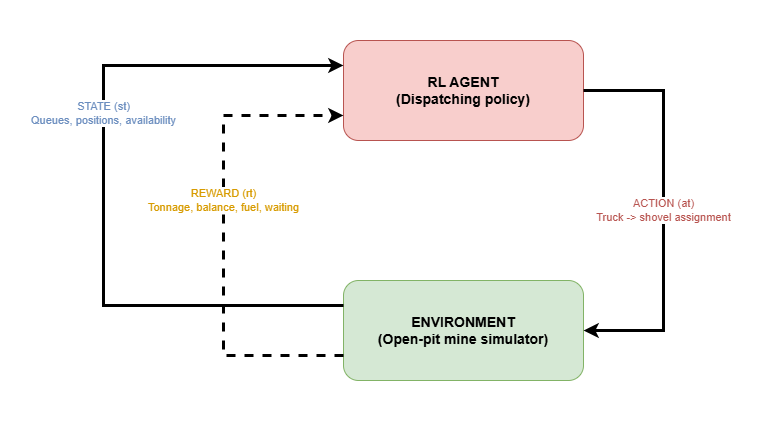
\includegraphics[width=0.9\textwidth]{figures/mdp_formulation.png}
\caption{Formulation du problème de dispatching de camions sous forme de processus de décision.}
\label{fig:mdp}
\end{figure}

\rev{m6}{\ifrevmarks\small Fichier renommé \texttt{mdp\_formulation.png} ; son contenu est déjà en anglais.\fi}

\subsection{Fonction de récompense multi-objectif}
\label{sec:reward}

\begin{revbloc}{M10, M16, v3}
L'objectif de l'agent est de maximiser la récompense cumulée actualisée sur un poste (\cref{eq:smdp-return}). La récompense d'un cycle $c$, décidé pour le camion $i$, vaut :

\begin{equation}
r_c = w_1\, r^{\mathrm{prod}}_c - w_2\, p^{\mathrm{éq}}_c - w_3\, c^{\mathrm{dist}}_c - w_4\, p^{\mathrm{att}}_c ,
\label{eq:reward}
\end{equation}

avec $w_1 = 1$, $w_2 = 0{,}1$, $w_3 = 0{,}05$ et $w_4 = 0{,}3$, et où :

\begin{itemize}
  \item $r^{\mathrm{prod}}_c = q_c / Q$ est la production du cycle, rapportée à la capacité $Q = 140$~t : elle vaut 1 si le cycle se termine avant la fin du poste et 0 sinon ;
  \item $p^{\mathrm{éq}}_c = \frac{1}{100}\,\mathrm{Var}_j\big(\omega_j\big)$ pénalise le déséquilibre entre pelles, où $\omega_j$ est le temps restant, en minutes, avant que la pelle $j$ soit libre au moment de la décision ;
  \item $c^{\mathrm{dist}}_c = \big(d(x_i, j) + d(j, k)\big)/5$ est la distance du cycle en kilomètres, divisée par 5, où $x_i$ est le lieu du camion (parc ou verse), $j$ la pelle et $k$ la verse choisies ; le retour à vide est le premier trajet du cycle suivant ;
  \item $p^{\mathrm{att}}_c = \min\big((W^{\mathrm{pelle}}_c + W^{\mathrm{verse}}_c)/30\,;\,1\big)$ pénalise l'attente en file réellement subie pendant le cycle, en minutes, divisée par 30 et plafonnée à 1.
\end{itemize}

\textbf{Moment du versement.} La récompense d'un cycle n'est connue qu'à sa fin, puisque les files dépendent des arrivées des autres camions. Elle est versée au pas pendant lequel le cycle se termine. La récompense $R_t$ d'un pas est donc la somme des récompenses des cycles terminés depuis la décision précédente, quel que soit le camion, augmentée du coût d'une ATTENDRE si c'est l'action choisie. À la fin du poste, les cycles en cours sont menés à terme : la somme des $R_t$ sur un poste est la somme des récompenses de tous ses cycles. Une version où la récompense était estimée et versée au moment de la décision a été essayée puis rejetée pendant la mise au point (\cref{sec:tuning}).

\textbf{Coût d'une attente volontaire.} Pour l'action ATTENDRE, de durée $\delta_t$, la récompense vaut
\begin{equation}
R^{\mathrm{att}}_t = - w_4 \min(\delta_t/30\,;\,1) - w_1\, \frac{\delta_t}{23{,}2} .
\label{eq:wait-reward}
\end{equation}
Le second terme est le coût d'opportunité de l'immobilité : la production perdue par un camion arrêté, en cycles, où 23,2~min est la durée moyenne d'un cycle de l'Affectation fixe en conditions nominales. Il est pondéré par $w_1$, car il s'exprime dans la même unité que la production, et n'ajoute donc aucun poids à régler. Dans la version précédente, ce terme n'existait pas : une attente de 0,2~min ne coûtait qu'environ 0,002, et PPO choisissait ATTENDRE dans 87\,\% de ses décisions en forte charge. Les politiques qui n'attendent jamais, dont toutes les heuristiques, ont exactement la même récompense qu'avec la formulation précédente.

\textbf{Ordre de grandeur.} Avec ces normalisations, la récompense cumulée d'un poste est proche du nombre de cycles terminés, diminué principalement du coût de distance. Pour l'Affectation fixe en conditions nominales (moyenne sur les 10 graines de sélection, \cref{sec:protocol}), 241,5 cycles livrés donnent une récompense de 218,7, dont $-19{,}3$ pour la distance, $-2{,}1$ pour l'équilibre et $-1{,}4$ pour l'attente.

\textbf{Récompense non modifiée.} La récompense a été fixée avant la campagne. Une variante qui étendait le coût d'opportunité à tous les cycles a été essayée pendant la mise au point, puis abandonnée (\cref{sec:tuning}). Le défaut qu'elle visait a été corrigé par l'actualisation par minute (\cref{sec:discount}), sans changer la récompense.
\end{revbloc}

Les poids privilégient la production tout en conservant une pénalité d'attente. La sensibilité des agents à $w_4$ est examinée dans l'étude d'ablation (\cref{sec:ablation}).

\subsection{Agents d'apprentissage étudiés}
\label{sec:agents}

\subsubsection{Proximal Policy Optimization}

PPO \cite{JohnSchulman2017} est un algorithme acteur--critique qui optimise directement la politique. Son objectif utilise une fonction de substitution écrêtée afin d'éviter des mises à jour de politique trop importantes :

\begin{equation}
L^{\mathrm{CLIP}}(\theta) = \hat{\mathbb{E}}_t \Big[ \min \big( r_t(\theta)\hat{A}_t,\ \mathrm{clip}(r_t(\theta), 1-\epsilon, 1+\epsilon)\hat{A}_t \big) \Big],
\qquad r_t(\theta) = \frac{\pi_\theta(a_t \mid s_t)}{\pi_{\theta_{\mathrm{old}}}(a_t \mid s_t)} ,
\end{equation}

\rev{Bibliographie, v3}{où l'avantage $\hat{A}_t$ est estimé par la méthode d'estimation généralisée de l'avantage (Generalized Advantage Estimation, GAE) \cite{Schulman2016GAE}, avec le facteur par minute de la \cref{sec:discount}.} L'acteur et le critique sont deux perceptrons multicouches distincts comportant chacun deux couches cachées de 128 neurones et une activation tangente hyperbolique, valeur par défaut de Stable-Baselines3 pour PPO ; la couche de sortie de l'acteur définit une distribution sur les 7 actions. \rev{v3}{La récompense est normalisée pendant l'entraînement (\texttt{VecNormalize} de Stable-Baselines3, observations non normalisées, puisqu'elles sont déjà dans $[0,1]$). Un seul environnement simulé est utilisé.}

\begin{revbloc}{M12, v3}
Les hyperparamètres sont rassemblés dans le \cref{tab:hyper}. Pour PPO et DQN, le taux d'apprentissage et, selon l'algorithme, le coefficient d'entropie ou la durée de l'exploration ont été choisis par un réglage de même taille pour les deux agents : quatre configurations chacun, valeurs de la version précédente incluses, 200\,000 pas, graine d'entraînement 1, critère de productivité sur les graines de sélection. Le facteur $\gamma = 0{,}995$ et la normalisation de la récompense de PPO ont été retenus pendant la mise au point des agents (\cref{sec:tuning}). Le même $\gamma$ a été donné à DQN, mais pas la normalisation : sa mémoire de rejeu conserverait des récompenses normalisées avec des statistiques qui changent pendant l'entraînement. Pour Q-Learning et SARSA, le taux d'apprentissage et le nombre d'intervalles de discrétisation ont été choisis par un réglage de même taille (quatre configurations chacun, budget complet). Leur facteur $\gamma = 0{,}99$ est celui de la version précédente : la règle de mise au point gardait la configuration des agents tabulaires en dehors de ce réglage. Les autres valeurs reprennent les valeurs par défaut de Stable-Baselines3 et les réglages usuels \cite{JohnSchulman2017, Mnih2015}.

Les budgets d'entraînement sont exprimés dans des unités différentes : les méthodes tabulaires sont entraînées pendant 30\,000 épisodes, chaque épisode comptant environ 250 décisions, et les agents profonds pendant 2~millions de décisions, soit environ 8\,000 postes. Les deux budgets ne sont pas directement comparables.
\end{revbloc}

\begin{table}[H]
\centering
\caption{\rev{M12, v3}{Hyperparamètres des algorithmes d'apprentissage. Les valeurs choisies par un réglage sont en gras.}}
\label{tab:hyper}
\footnotesize
\setlength{\tabcolsep}{4pt}
\begin{tabular}{lcccc}
\toprule
\textbf{Hyperparamètre} & \textbf{PPO} & \textbf{DQN} & \textbf{Q-Learning} & \textbf{SARSA} \\
\midrule
Représentation                 & MLP [128, 128] & MLP [128, 128] & \multicolumn{2}{c}{table, 6 variables (\cref{sec:tabular})} \\
Activation                     & Tanh$^{a}$     & ReLU$^{a}$     & s.o. & s.o. \\
Intervalles de discrétisation  & s.o. & s.o. & \textbf{6} & \textbf{6} \\
Taux d'apprentissage $\alpha$  & $\mathbf{1\times10^{-4}}$ & $\mathbf{3\times10^{-4}}$ & \textbf{0,2} & \textbf{0,1} \\
Facteur $\gamma$ (décision de 1,89~min) & 0,995 & 0,995 & 0,99 & 0,99 \\
Actualisation                  & \multicolumn{4}{c}{par minute, $\gamma_{\min} = \gamma^{1/1{,}89}$ (\cref{sec:discount})} \\
Normalisation de la récompense & oui & non & non & non \\
Taille de lot                  & 64             & 64             & s.o. & s.o. \\
$n_{\mathrm{steps}}$ / $n_{\mathrm{epochs}}$ & 1\,024 / 10 & s.o. & s.o. & s.o. \\
GAE $\lambda$ / écrêtage $\epsilon$ & 0,95 / 0,2 & s.o. & s.o. & s.o. \\
Coefficient d'entropie         & \textbf{0}     & s.o. & s.o. & s.o. \\
Tampon de rejeu / échauffement & s.o. & 200\,000 / 1\,000 & s.o. & s.o. \\
Mise à jour du réseau cible    & s.o. & tous les 1\,000 pas & s.o. & s.o. \\
Exploration $\varepsilon$      & s.o. & $1\to0{,}02$, \textbf{10\,\%} des pas & \multicolumn{2}{c}{$1\to0{,}01$, sur les épisodes} \\
Budget d'entraînement          & 2\,000\,000 pas & 2\,000\,000 pas & 30\,000 épisodes & 30\,000 épisodes \\
\bottomrule
\end{tabular}
\\[4pt]
\raggedright
\footnotesize $^{a}$\,Valeur par défaut de la bibliothèque SB3 : Tanh pour les algorithmes on-policy (PPO) ; ReLU pour les algorithmes off-policy (DQN).\\
\end{table}

\subsubsection{Deep Q-Network}

\rev{Bibliographie, M14, v3}{DQN \cite{Mnih2015} approxime la fonction de valeur action $Q(s,a)$ par un réseau de neurones, et stabilise l'apprentissage par un tampon de rejeu d'expériences et un réseau cible mis à jour périodiquement. Avec l'actualisation par minute, la mise à jour vise la cible}
\begin{equation}
y = r + \gamma_{\min}^{\Delta t} \max_{a'} Q_{\theta^-}(s', a') ,
\end{equation}
\rev{v3}{où $\Delta t$ est la durée de la décision, conservée avec chaque transition dans le tampon de rejeu.} Le réseau comporte deux couches cachées de 128 neurones avec une activation ReLU. \rev{v3}{L'exploration suit une stratégie $\varepsilon$-gloutonne dont le taux décroît linéairement de 1,0 à 0,02 sur les 10\,\% premiers pas d'entraînement.}

\subsubsection{Agents tabulaires : Q-Learning et SARSA}
\label{sec:tabular}

\begin{revbloc}{M8, v3}
Q-Learning \cite{WatkinsDayan1992} et SARSA \cite{RummeryNiranjan1994} stockent une valeur pour chaque couple état--action dans une table. L'état de 23 composantes étant trop grand pour une table, il est réduit à six variables. Les cinq premières sont les temps d'attente aux 3 pelles et aux 2 verses, découpés en 6 intervalles égaux entre 0 et 9,6~min (au-delà, la valeur sature). La sixième est \pending{selon les essais 24 et 25 : l'indice de la pelle la plus proche du camion qui décide (0 à 2), ou celui de la route de plus petite attente prévue (0 à 5), lu dans le bloc des attentes prévues par route}. L'espace discrétisé compte donc \pending{$6^5 \times 3 = 23\,328$ ou $6^5 \times 6 = 46\,656$} états. Lorsqu'un état est absent de la table, l'action 0 est jouée par défaut ; la part des décisions concernées est mesurée pendant l'évaluation. Cette représentation ne dépend pas du nombre de camions.

Q-Learning met à jour la valeur de l'action à partir de la meilleure action suivante (méthode hors politique), tandis que SARSA utilise l'action effectivement choisie ensuite (méthode sur politique). Avec l'actualisation par minute, la mise à jour s'écrit
\begin{equation}
Q(s,a) \leftarrow Q(s,a) + \alpha \big[ r + \gamma_{\min}^{\Delta t}\, Q(s',a') - Q(s,a) \big] ,
\end{equation}
où $a'$ est l'action de plus grande valeur en $s'$ pour Q-Learning, et l'action choisie en $s'$ pour SARSA. Les deux agents utilisent $\gamma = 0{,}99$ et une exploration $\varepsilon$-gloutonne décroissant linéairement de 1,0 à 0,01 sur 30\,000 épisodes. Q-Learning utilise $\alpha = 0{,}2$ et SARSA $\alpha = 0{,}1$, valeurs choisies par le réglage (\cref{sec:tuning}). La comparaison entre agents tabulaires et profonds doit donc être lue avec la représentation et le budget de calcul retenus ici.
\end{revbloc}

Les Algorithmes~\ref{alg:ppo}, \ref{alg:dqn} et \ref{alg:qlearning} formalisent les méthodes d'apprentissage sous forme de pseudocode ; la ligne qui distingue SARSA de Q-Learning est indiquée à la fin de l'Algorithme~\ref{alg:qlearning}. \rev{v3}{Dans les trois, $\Delta t_t$ est la durée de la décision $t$, donnée par le simulateur, et $\gamma_{\min} = \gamma^{1/1{,}89}$.}

\begin{algorithm}[H]
\caption{PPO pour le dispatching de camions miniers}
\label{alg:ppo}
\begin{algorithmic}[1]
\Require Environnement minier $\mathcal{E}$ ; acteur $\pi_\theta$ et critique $V_\phi$ (MLP $[128,128]$, Tanh)
\Require $\alpha{=}10^{-4}$, $\gamma{=}0{,}995$, $\lambda_{\text{GAE}}{=}0{,}95$, $\epsilon_{\text{clip}}{=}0{,}2$, $N{=}1024$, $T_{\max}{=}2{\times}10^6$
\State Initialiser $\theta$, $\phi$ aléatoirement ; $\gamma_{\min}\leftarrow\gamma^{1/1{,}89}$
\For{$k = 1,2,\ldots,\lfloor T_{\max}/N\rfloor$}
  \For{$t = 1,\ldots,N$} \Comment{Collecter le déroulement}
    \State Observer $s_t$ (\cref{tab:state})
    \State Échantillonner $a_t \sim \pi_\theta(\cdot\mid s_t)$, $\;a_t\in\{0,\ldots,6\}$ (couple pelle--verse ou \textsc{attendre})
    \State Exécuter $a_t$ ; recevoir $r_t$ (cycles terminés pendant le pas, \cref{eq:reward}), $s_{t+1}$ et la durée $\Delta t_t$
    \State Normaliser $r_t$ ; stocker $\bigl(s_t,\,a_t,\,r_t,\,\gamma_{\min}^{\Delta t_t},\,\log\pi_\theta(a_t\mid s_t)\bigr)$
  \EndFor
  \State Calculer les avantages : $\hat{A}_t = \delta_t + \gamma_{\min}^{\Delta t_t}\lambda_{\text{GAE}}\hat{A}_{t+1}$,
         $\;\delta_t = r_t + \gamma_{\min}^{\Delta t_t} V_\phi(s_{t+1}) - V_\phi(s_t)$
  \For{chaque époque, mini-lots de taille 64}
    \State $r_t(\theta)\leftarrow \pi_\theta(a_t\mid s_t)/\pi_{\theta_k}(a_t\mid s_t)$
    \State Maximiser $L^{\text{CLIP}}(\theta)=\mathbb{E}\bigl[\min\bigl(r_t\hat{A}_t,\;\mathrm{clip}(r_t,1{-}\epsilon_{\text{clip}},1{+}\epsilon_{\text{clip}})\hat{A}_t\bigr)\bigr]$
    \State Minimiser $L^{V}(\phi)=\mathbb{E}\bigl[(V_\phi(s_t)-R_t^{\text{target}})^2\bigr]$
  \EndFor
\EndFor
\Ensure Politique entraînée $\pi_\theta^*$
\end{algorithmic}
\end{algorithm}

\begin{algorithm}[H]
\caption{DQN pour le dispatching de camions miniers}
\label{alg:dqn}
\begin{algorithmic}[1]
\Require $\mathcal{E}$ ; réseaux $Q_\theta$, $Q_{\theta^-}$ (MLP $[128,128]$, ReLU) ; tampon de rejeu $\mathcal{B}$ (200\,000)
\Require $\alpha{=}3{\times}10^{-4}$, $\gamma{=}0{,}995$, $\varepsilon{:}\;1{,}0\!\to\!0{,}02$ (linéaire sur $10\,\%$ des pas)
\State Initialiser $\theta$ aléatoirement ; $\theta^-\leftarrow\theta$ ; $\mathcal{B}\leftarrow\emptyset$ ; $\gamma_{\min}\leftarrow\gamma^{1/1{,}89}$
\For{chaque pas $t = 1,2,\ldots,T_{\max}$}
  \State Avec prob.\ $\varepsilon$ : $a_t\sim\text{Uniform}(\mathcal{A})$ ; sinon $a_t\leftarrow\arg\max_a Q_\theta(s_t,a)$
  \State Exécuter $a_t$ ; observer $r_t$, $s_{t+1}$, $\Delta t_t$ ; stocker $(s_t,a_t,r_t,s_{t+1},\gamma_{\min}^{\Delta t_t})$ dans $\mathcal{B}$
  \State Échantillonner un mini-lot $\{(s_i,a_i,r_i,s'_i,d_i)\}$ depuis $\mathcal{B}$
  \State $y_i \leftarrow r_i + d_i\max_{a'}Q_{\theta^-}(s'_i,a')$ \Comment{Cible actualisée par la durée de la décision}
  \State Minimiser $\frac{1}{B}\sum_i\bigl(Q_\theta(s_i,a_i)-y_i\bigr)^2$
  \If{$t \bmod 1000 = 0$} $\theta^-\leftarrow\theta$ \EndIf \Comment{Synchroniser le réseau cible}
\EndFor
\Ensure $\pi(s)=\arg\max_a Q_\theta(s,a)$
\end{algorithmic}
\end{algorithm}

\begin{algorithm}[H]
\caption{Q-Learning pour le dispatching de camions miniers (référence tabulaire)}
\label{alg:qlearning}
\begin{algorithmic}[1]
\Require $\mathcal{E}$ ; $\alpha{=}0{,}2$ (SARSA : 0,1), $\gamma{=}0{,}99$, $\varepsilon{:}\;1{,}0\!\to\!0{,}01$ (linéaire sur 30\,000 épisodes)
\State Initialiser $Q(s,a)\leftarrow 0$ pour tout $(s,a)$ (état réduit à 6 variables, 6 intervalles) ; $\gamma_{\min}\leftarrow\gamma^{1/1{,}89}$
\For{épisode $= 1, \ldots, 30\,000$}
  \State $s_0\leftarrow\texttt{reset}(\mathcal{E})$
  \While{l'épisode n'est pas terminé}
    \State Avec prob.\ $\varepsilon$ : $a_t\sim\text{Uniform}(\mathcal{A})$ ; sinon $a_t\leftarrow\arg\max_a Q(s_t,a)$
    \State Exécuter $a_t$ ; observer $r_t$, $s_{t+1}$, $\Delta t_t$
    \State $Q(s_t,a_t)\leftarrow Q(s_t,a_t)+\alpha\bigl[r_t+\gamma_{\min}^{\Delta t_t}\max_{a'}Q(s_{t+1},a')-Q(s_t,a_t)\bigr]$
    \State $s_t\leftarrow s_{t+1}$
  \EndWhile
  \State Décroître $\varepsilon$ linéairement
\EndFor
\Ensure $\pi^*(s)=\arg\max_a Q(s,a)$
\Statex \textbf{Note (SARSA) :} remplacer $\max_{a'}Q(s_{t+1},a')$ par $Q(s_{t+1},a_{t+1})$ pour des mises à jour on-policy.
\end{algorithmic}
\end{algorithm}

\subsection{Heuristiques de référence}
\label{sec:baselines-def}

\begin{revbloc}{M25, M16, Dir. corr. 1, A, v3}
Les six règles de référence sont définies dans le \cref{tab:baselines} telles qu'elles sont implémentées. Aucune n'utilise l'action ATTENDRE. Elles se répartissent en trois groupes.

\textbf{Règles tenant compte des files et des trajets.} La règle du temps d'attente minimal des camions (MTWT) envoie le camion à la pelle où il attendra le moins à son arrivée, en combinant le temps de trajet moyen et la libération prévue de chaque pelle, camions déjà en route compris ; elle choisit la verse de la même façon. Elle représente les règles des systèmes commerciaux de gestion de flotte \cite{Zeng2022}. La politique fondée sur un programme linéaire (LP) suit le principe de DISPATCH \cite{Soumis1989} : un programme linéaire fixe, en début de poste, des taux de flux cibles sur chaque route pelle--verse ; à chaque décision, le camion est envoyé sur la route la plus en retard sur son plan. Le programme maximise la production sous des contraintes de capacité des pelles et des verses, de conservation des camions et d'heures-camions disponibles, en limitant l'utilisation planifiée de chaque ressource à une valeur $u \leq 1$. Avec $u = 1$, le plan sature la pelle la plus proche, ce qui est optimal sans aléa mais crée une file sans limite avec des durées aléatoires. La valeur $u = 0{,}7$ a été choisie parmi sept candidats sur les graines de sélection, jamais sur celles de l'évaluation, et sert pour les trois régimes. Ces deux règles n'utilisent que des grandeurs moyennes (temps de trajet, durées de service, probabilité de panne), jamais les aléas de l'épisode.

\textbf{Règles tenant compte des files seulement, ou d'aucune information.} La règle appelée FIFO dans la version précédente choisit la pelle qui sera libre le plus tôt, sans tenir compte des trajets : une pelle libre dans une minute mais lointaine passe avant une pelle proche libre dans deux minutes. Ce n'est donc pas une file « premier arrivé, premier servi » ; le nom est conservé pour la continuité avec la version précédente. L'Affectation fixe attache chaque camion à une pelle et à une verse pendant tout le poste, sans réaffectation.

\textbf{Règles géométriques.} La Pelle la plus proche et le Plus court chemin ignorent les files. Depuis que la décision est prise à la verse, ils comparent réellement toutes les pelles. Mais la pelle 1 est la plus proche du parc et des deux verses : la Pelle la plus proche y envoie toute la flotte pendant tout le poste, et sa production est plafonnée par la capacité d'une seule pelle (environ 4\,200~t/h). Le Plus court chemin, dont le coût compte aussi le trajet pelle--verse, envoie environ 72\,\% de ses cycles à cette pelle. Ces deux règles sont des bornes basses, et non des représentants de la pratique industrielle.
\end{revbloc}

\begin{table}[H]
\centering
\caption{\rev{M25, Dir. corr. 1, v3}{Définition des heuristiques de référence telles qu'implémentées.}}
\label{tab:baselines}
\small
\begin{tabularx}{\textwidth}{lX}
\toprule
\textbf{Politique} & \textbf{Règle appliquée lorsque le camion $i$ devient disponible} \\
\midrule
MTWT & Pour chaque pelle $j$ : arrivée prévue $a_j = t + $ trajet moyen à vide ; attente prévue $\max(0,\ \text{libération prévue de } j - a_j)$. Choisir la pelle de plus petite attente (à égalité, la plus tôt atteinte), puis la verse de la même façon, depuis la fin prévue du chargement. \\
LP (programme linéaire) & En début de poste, taux de flux cibles $x_{jk}$ (cycles/h) maximisant la production, utilisation planifiée $\leq u = 0{,}7$. À chaque décision : la route dont le nombre de cycles lancés est le plus en retard sur $x_{jk}$, à l'heure d'arrivée prévue à la pelle ; à égalité, la pelle la plus proche. \\
FIFO & Affecter le camion à la pelle qui sera libre le plus tôt et à la verse qui sera libre le plus tôt, indépendamment des distances. \\
Affectation fixe & Affecter le camion $i$ à la pelle $i \bmod 3$ et à la verse $i \bmod 2$ pendant tout le poste, sans réaffectation. \\
Pelle la plus proche & Affecter le camion à la pelle la plus proche de sa position sur le graphe, puis à la verse la plus proche de cette pelle, sans tenir compte des files. \\
Plus court chemin & Affecter le camion au couple pelle--verse qui minimise le coût $C = 0{,}5\,T + 0{,}3\,D + 0{,}2\,E/6{,}49$ des trajets camion--pelle et pelle--verse, où $T$, $D$ et $E$ sont le temps moyen, la distance et la consommation, calculés par l'algorithme de Dijkstra ; la division par 6,49 annule l'effet de la calibration du carburant sur les décisions. \\
\bottomrule
\end{tabularx}
\end{table}

\subsection{Architecture du système et coût de calcul}
\label{sec:compute}

L'architecture découple la logique d'apprentissage de la simulation, ce qui permet de tester différents agents de manière interchangeable (\cref{fig:architecture}). L'agent sélectionne une action $a_t$ à partir de l'état $s_t$ ; l'environnement applique l'affectation et renvoie l'état suivant et la récompense ; le module d'évaluation calcule les indicateurs pour \rev{v3}{les dix politiques (six heuristiques et quatre agents)} dans les trois régimes.

\begin{figure}[H]
\centering
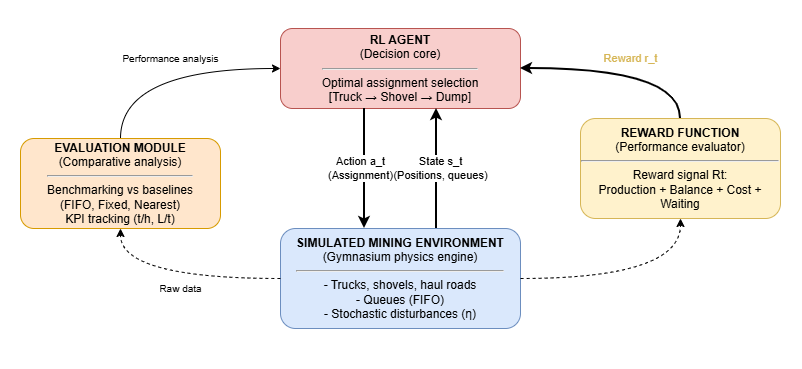
\includegraphics[width=0.88\textwidth]{figures/functional_architecture.png}
\caption{Boucle d'interaction entre l'agent et l'environnement.}
\label{fig:architecture}
\end{figure}

\rev{m6}{\ifrevmarks\small Fichier renommé \texttt{functional\_architecture.png} ; son contenu est déjà en anglais.\fi}

\begin{revbloc}{M28, m20, m24, v3}
Toutes les mesures sont faites sur le processeur d'un ordinateur portable à 8 cœurs, sans carte graphique.
\begin{itemize}
  \item \textbf{Entraînement :} un entraînement complet en conditions nominales, avec quatre entraînements en même temps sur la machine, a duré 223~min pour PPO, 168~min pour DQN, 253~min pour Q-Learning et 241~min pour SARSA. Chaque entraînement utilise un seul environnement simulé, exigence de l'actualisation par minute (\cref{sec:discount}). Collecter avec quatre environnements en parallèle n'accélérerait PPO que d'un facteur 1,47 et changerait le modèle obtenu (4\,096 pas par mise à jour au lieu de 1\,024) : ce choix n'a pas été retenu. L'entraînement est déterministe pour une graine donnée. La campagne complète compte 60 entraînements (4 algorithmes, 3 régimes, 5 graines), pour une durée totale de \pending{durée mesurée pendant la campagne}.
  \item \textbf{Évaluation :} chaque épisode d'évaluation ne dépend que de la politique et de sa graine, grâce aux flux aléatoires séparés (\cref{sec:simulator}). Les épisodes sont donc répartis entre plusieurs processus, avec exactement les mêmes résultats qu'en séquentiel, graine par graine. Sur 150 épisodes, 4 processus divisent la durée par 2 ; 8 processus font moins bien que 4, car chacun doit d'abord charger PyTorch.
  \item \textbf{Inférence :} la latence d'une décision, construction de l'état comprise, est inférieure à 1~milliseconde pour toutes les politiques : de 0,48 à 0,71~ms pour PPO et de 0,36 à 0,49~ms pour DQN, de 12 à 24 camions. Comme l'état a une taille fixe, elle dépend peu de la taille de la flotte. Elle est négligeable devant la durée d'un cycle de transport, mais son adéquation aux contraintes d'un système de gestion de flotte commercial n'a pas été évaluée.
  \item \textbf{Mémoire :} \pending{taille des fichiers des modèles de la campagne}.
\end{itemize}
\end{revbloc}

\adir{adéquation de la revue cible (Cluster Computing) si la dimension calcul reste limitée (M28).}


% ============================================================================
% Section 6 : Plan expérimental
% ============================================================================
\section{Plan expérimental}
\label{sec:design}

Cette section détaille les régimes de fonctionnement, le protocole d'entraînement et d'évaluation, les indicateurs et le cadre statistique.

\subsection{Régimes de fonctionnement}
\label{sec:scenarios}

Trois régimes sont définis (\cref{tab:scenarios,fig:scenarios}). Chaque épisode correspond à un poste de 8~heures (480~minutes).

\begin{revbloc}{M15}
Pour situer chaque régime par rapport à la capacité de chargement, nous utilisons le facteur d'appariement \cite{BurtCaccetta2014} :
\begin{equation}
\mathrm{MF} = \frac{N \times t_{\mathrm{chargement}}}{S \times t_{\mathrm{cycle}}} ,
\label{eq:mf}
\end{equation}
où $N$ est le nombre de camions, $S$ le nombre de pelles, $t_{\mathrm{chargement}} = 2$~min la durée moyenne de chargement et $t_{\mathrm{cycle}} \approx 22{,}7$~min la durée moyenne d'un cycle hors attente et hors panne, mesurée avec l'Affectation fixe. Un facteur inférieur à 1 indique que les pelles attendent les camions. Il vaut environ 0,35 en conditions nominales et 0,52 en forte charge : même avec 18 camions, la flotte reste en dessous de la capacité des trois pelles, qui peuvent charger ensemble environ 12\,600~t/h. Le régime de forte charge augmente donc la pression sur les files, mais ne constitue pas une sursaturation de la flotte ; seule une politique qui concentre les camions sur une seule pelle peut saturer celle-ci.
\end{revbloc}

\begin{table}[H]
\centering
\caption{Paramètres des trois régimes de fonctionnement.}
\label{tab:scenarios}
\footnotesize
\setlength{\tabcolsep}{4pt}
\begin{tabular}{lcccccl}
\toprule
\textbf{Régime} & \textbf{Camions} & \textbf{Pelles} & \textbf{Verses} & \textbf{Pannes par cycle} & \textbf{MF} & \textbf{Caractéristique} \\
\midrule
Nominal        & 12 & 3 & 2 & 2\,\%  & \rev{M15}{0,35} & Conditions de référence \\
Forte charge   & 18 & 3 & 2 & 2\,\%  & \rev{M15}{0,52} & \rev{M15}{Flotte augmentée de 50\,\%} \\
Fortes pannes  & 12 & 3 & 2 & 10\,\% & \rev{M15}{0,35} & Pannes de camions fréquentes \\
\bottomrule
\end{tabular}
\end{table}

\begin{figure}[H]
\centering
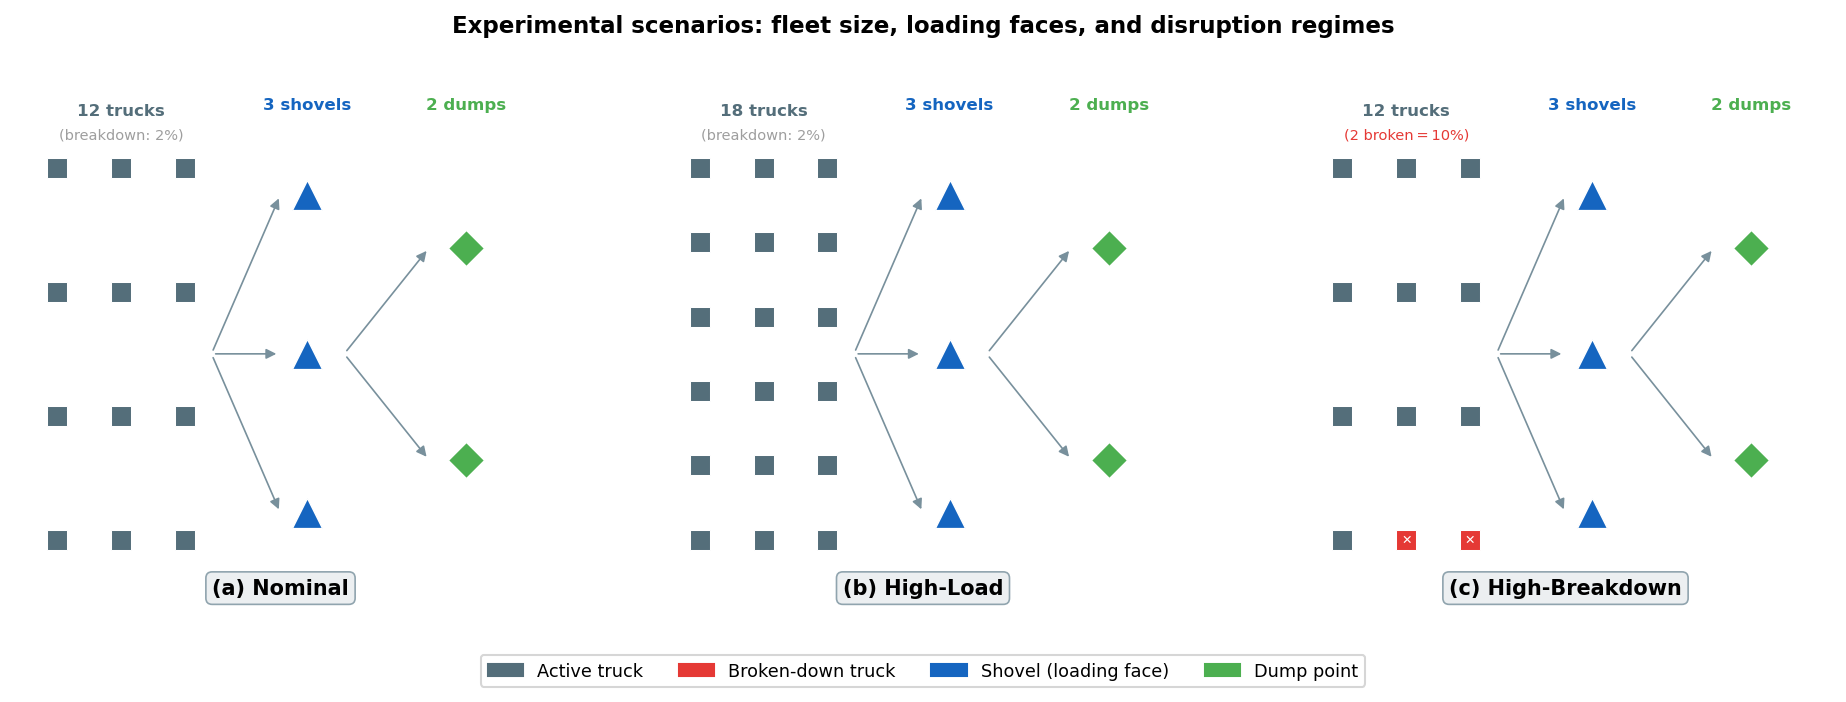
\includegraphics[width=0.95\textwidth]{figures/fig3_scenarios.png}
\caption{Configuration des trois régimes de fonctionnement.}
\label{fig:scenarios}
\end{figure}

\subsection{Protocole d'entraînement et d'évaluation}
\label{sec:protocol}

\begin{revbloc}{M1, M7, m19, A, v3}
\textbf{Trois ensembles de graines disjoints.} Les graines d'évaluation (42 à 71) donnent les 30 réplications de chaque résultat. Les graines de sélection (20\,000 à 20\,009) ont servi à tous les choix faits avant la campagne : réglage des hyperparamètres, choix de $u$ pour la politique LP et mise au point des agents (\cref{sec:tuning}). Les graines d'entraînement (1 à 5) initialisent les agents ; l'agent de graine $s$ joue ses épisodes d'entraînement sur les graines $s \times 10^6, s \times 10^6 + 1, \ldots$, qui ne croisent jamais les deux autres ensembles. Un test vérifie, pour les quatre algorithmes, que toutes les graines utilisées pendant un entraînement sont des graines d'entraînement. Aucun choix n'a été fait sur les graines d'évaluation, et aucun agent n'y a été évalué avant la campagne finale ; rien n'a été modifié après avoir vu ses résultats. Dans la version précédente, les graines d'évaluation étaient aussi les premiers épisodes d'entraînement.

\textbf{Agents spécialisés.} Chaque agent d'apprentissage est entraîné dans chacun des trois régimes avec 5 graines d'entraînement : 2~millions de pas pour PPO et DQN, 30\,000 épisodes pour Q-Learning et SARSA, soit 60 entraînements. Les résultats principaux comparent, dans chaque régime, les agents entraînés dans ce régime aux six heuristiques.

\textbf{Évaluation sans réentraînement.} Pour mesurer la capacité d'une politique apprise à supporter un changement de régime, les agents entraînés en conditions nominales sont en outre évalués, sans aucun réentraînement, en forte charge et en fortes pannes, sur les mêmes graines que les agents spécialisés. C'est possible pour les quatre agents, puisque l'état a la même taille quel que soit le nombre de camions (\cref{sec:smdp}). Les agents nominaux sont aussi évalués dans deux régimes intermédiaires jamais vus : 15 camions avec 2\,\% de pannes, et 12 camions avec 5\,\% de pannes.

\textbf{Évaluation.} Toutes les politiques sont évaluées sur les mêmes 30 réplications. Les agents choisissent l'action de plus grande valeur, sans exploration : mode déterministe pour PPO, $\varepsilon = 0$ pour DQN et choix glouton pour les agents tabulaires.

\textbf{Deux sources de variabilité.} Les 30 réplications mesurent la variabilité due à l'environnement ; les 5 graines d'entraînement mesurent celle due à l'apprentissage. Les deux sont rapportées séparément (\cref{sec:proto}).
\end{revbloc}

\subsection{Mise au point des agents}
\label{sec:tuning}

\begin{revbloc}{M7, M12, v3}
Après les corrections du simulateur (moteur à événements, décision à la verse), les agents réglés selon la procédure de la version précédente faisaient moins bien qu'une politique au hasard. Plusieurs essais ont alors été faits pour comprendre et améliorer l'apprentissage. Multiplier les essais jusqu'à ce que l'apprentissage par renforcement dépasse les heuristiques serait un biais : chaque essai est une chance de tomber par hasard sur une version favorable. Cette section décrit donc la règle suivie et rapporte \emph{tous} les essais, y compris ceux qui ont échoué.

\textbf{Règle.} Elle a été écrite et datée avant les essais qu'elle encadre, et complétée avant chaque nouvelle étape :
\begin{itemize}
  \item tous les essais se font en conditions nominales, avec la graine d'entraînement 1, et sont jugés sur la productivité moyenne de la politique sans exploration sur les graines de sélection ; les graines d'évaluation ne servent jamais ;
  \item chaque étape est fixée à l'avance, avec son critère de décision, et une variante n'est retenue que si elle fait mieux que la version précédente ;
  \item tout ce qui est retenu pour PPO s'applique à DQN quand cela a un sens, et les agents tabulaires reçoivent un réglage de même taille ;
  \item la liste des étapes est close : après la dernière, les agents partent en campagne quel que soit leur résultat, et ce résultat est présenté tel quel, même si les heuristiques restent devant.
\end{itemize}
Chaque essai est enregistré avec sa configuration et le commit du code utilisé, et peut être refait par une seule commande.

\textbf{Essais.} Le \cref{tab:tuning} les rapporte dans l'ordre. Les repères sur les mêmes graines sont : MTWT 4\,443~t/h, LP 4\,412, FIFO 4\,246, Affectation fixe 4\,226, politique au hasard 4\,167, Pelle la plus proche 3\,915.
\end{revbloc}

\begin{table}[H]
\centering
\caption{\rev{v3}{Essais de la mise au point des agents (productivité en t/h sur les graines de sélection 20\,000 à 20\,009, conditions nominales, graine d'entraînement 1). Entre parenthèses : la part des décisions ATTENDRE ou la part des cycles envoyés à une seule pelle, quand elle est remarquable.}}
\label{tab:tuning}
\scriptsize
\setlength{\tabcolsep}{3pt}
\begin{tabularx}{\textwidth}{>{\raggedright\arraybackslash}p{0.9cm}>{\raggedright\arraybackslash}X>{\raggedright\arraybackslash}p{4.6cm}>{\raggedright\arraybackslash}p{2.6cm}}
\toprule
\textbf{N\textsuperscript{o}} & \textbf{Essai} & \textbf{Résultat} & \textbf{Décision} \\
\midrule
\multicolumn{4}{l}{\emph{Actualisation par décision}} \\
0 & Réglage de PPO et DQN, 200\,000 pas & PPO 3\,953 (99\,\% pelle 1) ; DQN 3\,992 & point de départ \\
1, 2, 4 & Récompense estimée et versée à la décision, avec ou sans coût des minutes en file & PPO 3\,915 à 3\,981 ; DQN 4\,106 à 4\,191 (ATTENDRE 52 à 65\,\%) & rejetée \\
3 & PPO, budget complet, récompense versée à la fin du cycle & PPO 4\,260 & gardée \\
5 & Attente prévue par route dans l'état (23 composantes) & PPO 4\,345 & retenue \\
6 & Récompense normalisée et $\gamma = 0{,}995$ & PPO 4\,405 (ATTENDRE 36\,\%) & retenue \\
7 & Contrôle de DQN, budget complet, $\gamma = 0{,}995$ & DQN 3\,593 (99\,\% pelle 3) & gardé, sans variante \\
8, 9 & Q-Learning et SARSA, configuration de la version précédente & Q-Learning 3\,955 (62\,\% pelle 3) ; SARSA 3\,535 (98\,\% pelle 3) & point de départ \\
\midrule
\multicolumn{4}{l}{\emph{Coût d'opportunité étendu à tous les cycles (abandonné)}} \\
10--13 & Même configuration, récompense modifiée & PPO 210 (ATTENDRE 99,8\,\%) ; DQN 3\,532 (ATTENDRE 94,8\,\%) ; Q-Learning 4\,099 ; SARSA 4\,134 & abandonné \\
\midrule
\multicolumn{4}{l}{\emph{Actualisation par minute}} \\
14--17 & Même configuration que les essais 6 à 9 & PPO 4\,414 (ATTENDRE 0\,\%) ; DQN 121 (ATTENDRE 99,8\,\%) ; Q-Learning 3\,974 ; SARSA 3\,602 (100\,\% pelle 3) & PPO et DQN figés \\
16--23 & Réglage tabulaire : $\alpha \in \{0{,}1 ; 0{,}2\}$ × \{6 ; 8\} intervalles & Q-Learning 3\,369 à \textbf{4\,181} ($\alpha = 0{,}2$, 6 int.) ; SARSA 3\,481 à \textbf{3\,626} ($\alpha = 0{,}1$, 6 int.), 98 à 100\,\% pelle 3 & meilleures configurations \\
24, 25 & Sixième variable de l'état : route de plus petite attente prévue & \pending{résultats des essais 24 et 25} & \pending{retenue ou non} \\
\bottomrule
\end{tabularx}
\end{table}

\begin{revbloc}{v3}
\textbf{Ce qui a été retenu, et pourquoi.} Chaque changement retenu se justifie indépendamment de son score. Le bloc des attentes prévues par route donne à l'agent la même information que MTWT. La normalisation de la récompense et un horizon plus long sont des pratiques usuelles pour PPO. L'actualisation par minute corrige la formulation du problème (\cref{sec:discount}). Pendant la même période, les heuristiques de référence ont été renforcées : prévision des camions en route pour MTWT et FIFO, et ajout de la politique LP. La comparaison est donc devenue plus difficile pour l'apprentissage par renforcement.

\textbf{Le défaut trouvé, et la variante abandonnée.} Avec l'actualisation par décision, les trois agents à valeurs (DQN, Q-Learning, SARSA) dérivaient vers la pelle la plus éloignée, et leur productivité baissait à mesure que l'exploration diminuait. Une mesure sans réentraînement en a montré la cause. Aller toujours à la pelle 3 plutôt qu'à la pelle 1 fait perdre 9\,\% de productivité, mais ne change presque pas la récompense par décision (0,813 contre 0,820), car un cycle rapporte 1 quelle que soit sa durée. Une première correction, décidée avec la directrice de recherche, étendait le coût d'opportunité à tous les cycles (durée du cycle divisée par 23,2~min). La récompense d'un poste n'en changeait que d'une constante, et la dérive a disparu (essais 10 à 13). Mais un cycle rapportait alors en moyenne une valeur négative. Avec une actualisation par décision, repousser une récompense négative la rend moins coûteuse, et intercaler des attentes de 0,2~min devenait le moyen de la repousser. PPO a ainsi appris à attendre dans 99,8\,\% de ses décisions. Les deux défauts ont donc la même cause : une actualisation par décision alors que les décisions n'ont pas la même durée. Cette variante a été abandonnée, la récompense est revenue à sa définition précédente, et l'actualisation par minute a été introduite pour les quatre algorithmes, sans autre changement. Ces deux décisions ont été prises après avoir vu des résultats sur les graines de sélection : elles sont déclarées comme telles.

\textbf{L'effondrement de DQN.} Avec l'actualisation par minute, DQN choisit ATTENDRE dans 99,8\,\% de ses décisions (essai 15). Rejoué de façon gloutonne, le modèle final produit 840~t par poste, alors que les derniers postes d'entraînement, joués avec mises à jour et exploration, produisaient de 25\,620 à 30\,660~t. Notre interprétation, cohérente avec cette mesure mais non démontrée, est la suivante. Une attente de 0,2~min ne repousse la production suivante que de 0,2~min : sa valeur est donc presque égale à celle de la meilleure action, ce qui est juste. L'écart devient alors plus petit que l'erreur d'approximation du réseau. Dès que cette erreur place l'attente en tête, le modèle attend, et une attente en entraîne d'autres. PPO, qui apprend une politique et non des valeurs à comparer, n'est pas touché. Le test d'équivalence de la \cref{sec:discount} exclut une erreur d'implémentation. Conformément à la règle, DQN part en campagne dans cette version.
\end{revbloc}

\subsection{Indicateurs}
\label{sec:metrics}

\begin{revbloc}{M2, M21, M15, m18}
Dans cette étude, la résilience opérationnelle désigne la capacité d'une politique à conserver son débit et à contenir l'attente en file lorsque le système passe des conditions nominales à des conditions perturbées. Elle est mesurée par les indicateurs suivants, calculés pour chaque réplication.

\begin{enumerate}
  \item \textbf{Productivité :} tonnage livré par heure (t/h), et productivité par camion (t/h/camion), qui permet de comparer des régimes dont la flotte n'a pas la même taille.
  \item \textbf{Attente en file :} temps total passé par un camion en file d'attente aux pelles et aux verses pendant le poste, moyenné sur les camions (min par camion et par poste). Ce n'est pas une attente par cycle : avec environ 19 cycles par camion en conditions nominales, 22~min d'attente en file par poste correspondent à environ 1,1~min par cycle.
  \item \textbf{Temps d'immobilisation total :} somme, par camion et par poste, de l'attente en file, de l'immobilisation pour panne et du temps passé à attendre volontairement par l'action ATTENDRE. C'est l'indicateur rapporté sous le nom de « temps d'attente » dans la version précédente de cet article.
  \item \textbf{Utilisation des camions :} part du poste pendant laquelle les camions roulent, chargent ou déversent (\%). Le temps d'activité du dernier cycle qui dépasse la fin du poste est exclu.
  \item \textbf{Utilisation des pelles :} part du poste pendant laquelle les pelles chargent (\%).
  \item \textbf{Consommation spécifique :} carburant consommé par tonne livrée (L/t).
  \item \textbf{Nombre de cycles terminés} et \textbf{récompense cumulée} avec les poids de référence.
  \item \textbf{Ratio de robustesse :} rapport entre la performance dans un régime perturbé et la performance nominale :
  \begin{equation}
  \mathrm{RR}(p,s) = \frac{\mathrm{Performance}(p,s)}{\mathrm{Performance}(p,\mathrm{nominal})} .
  \label{eq:rr}
  \end{equation}
  En forte charge, ce ratio est calculé sur la productivité par camion, faute de quoi il refléterait surtout l'ajout de camions.
\end{enumerate}
\end{revbloc}

\subsection{Protocole statistique}
\label{sec:proto}

\begin{revbloc}{M3, M4, M5, M6, M7, M22, v3}
\textbf{Unité statistique.} Pour les comparaisons appariées, l'unité d'analyse est la réplication : chaque couple (politique, régime) fournit exactement 30 valeurs, une par graine d'évaluation. Pour un agent, la valeur d'une réplication est la moyenne de ses 5 modèles (un par graine d'entraînement) sur cette graine.

\textbf{Appariement.} La même graine est utilisée par toutes les politiques dans une réplication donnée, et le simulateur utilise un flux aléatoire séparé par processus et un flux de pannes par camion (\cref{sec:simulator}). Deux politiques jouées avec la même graine subissent donc les mêmes aléas : en particulier, le $k$-ième cycle d'un camion donné a la même panne, de même durée, quelle que soit la politique. Les observations sont appariées par graine, et les réplications sont traitées comme des blocs. Les temps de trajet et de service restent tirés dans l'ordre des événements, qui dépend des décisions : l'appariement est fort, sans être parfait.

\textbf{Tests.} Dans chaque régime, le test de Friedman \cite{Friedman1937} vérifie l'existence d'un effet de la politique. Les comparaisons par paires utilisent le test des rangs signés de Wilcoxon \cite{Wilcoxon1945}, bilatéral, avec une correction de Holm \cite{Holm1979} sur la famille des comparaisons rapportées dans chaque régime \cite{Demsar2006}. La dépendance du classement au régime (H2) est testée par un modèle linéaire de la productivité par camion comprenant la politique, les blocs (régime, graine) et l'interaction entre politique et régime.

\textbf{Tailles d'effet et intervalles.} Les différences sont rapportées en unités physiques, avec un intervalle de confiance bootstrap apparié à 95\,\% (10\,000 rééchantillonnages des différences par graine) \cite{EfronTibshirani1993}. Le $d$ de Cohen est rapporté à titre descriptif ; dans un simulateur, la variabilité entre réplications est faible, si bien qu'un $d$ élevé ne signifie pas un effet pratique important. Les valeurs $p$ inférieures à 0,001 sont rapportées sous la forme $p<0{,}001$.

\textbf{Variabilité d'entraînement.} Pour chaque agent et chaque régime, le score d'un modèle est sa moyenne sur les 30 graines d'évaluation. Les 5 modèles sont résumés par leur moyenne interquartile (IQM), avec un intervalle de confiance à 95\,\% par bootstrap stratifié par régime, ainsi que par le plus mauvais et le meilleur modèle \cite{Agarwal2021}. La probabilité d'amélioration $P(X > Y)$ entre deux agents est aussi rapportée. Pour l'agrégat sur les trois régimes, les scores sont divisés par la moyenne de l'Affectation fixe du même régime. Les courbes d'apprentissage sont la moyenne des 5 modèles évalués, avec un intervalle bootstrap point par point ; elles sont lues dans les journaux d'entraînement de ces modèles, et non dans des entraînements séparés.
\end{revbloc}

\subsection{Paramètres de reproductibilité}

\begin{revbloc}{M3, A}
La simulation est implémentée en Python 3.11.11 avec Gymnasium 1.2.3 \cite{MarkTowers2025}, Stable-Baselines3 2.8.0 \cite{AntoninRaffin2021} et PyTorch 2.5.1, sur processeur. Les poids de récompense ($w_1 = 1$, $w_2 = 0{,}1$, $w_3 = 0{,}05$, $w_4 = 0{,}3$) sont constants dans toutes les expériences, sauf dans l'étude d'ablation. \rev{v3}{Le facteur d'actualisation par minute est déduit de $\gamma$ et n'est jamais réglé (\cref{sec:discount}).} Les résultats par réplication, à raison d'une ligne par politique, régime et graine, sont fournis avec le code. Une version antérieure de l'analyse statistique avait été calculée sur un fichier de résultats dans lequel chaque réplication figurait deux fois, par suite de deux exécutions successives du banc d'essai ; toutes les valeurs $p$, tous les intervalles et tous les tests de cette version sont recalculés sur les 30 réplications uniques.
\end{revbloc}

\adir{la phrase sur la version antérieure de l'analyse est utile pour la directrice ; la retirer de la version soumise.}

\rev{N11, v3}{Tous les agents de cette version sont entraînés pendant la même campagne, avec le même simulateur et la même récompense. Chaque modèle est accompagné d'un fichier de métadonnées (version du code, hyperparamètres, durée d'entraînement), la configuration utilisée est archivée avec les résultats, et chaque essai de la mise au point peut être refait par une seule commande.}


% ============================================================================
% Section 7 : Résultats
% ============================================================================
\section{Résultats}
\label{sec:results}

Cette section présente la productivité, l'attente, le comportement des politiques, les compromis entre ces critères, la robustesse et le transfert sans réentraînement, puis la significativité statistique, la variabilité, la convergence et l'étude d'ablation. \rev{M3}{Toutes les statistiques sont calculées sur les 30 réplications uniques de chaque couple (politique, régime).}

\subsection{Productivité}
\label{sec:productivity}

Le \cref{tab:productivity} rapporte la productivité moyenne des huit politiques dans les trois régimes, ainsi que la productivité par camion. \rev{m16}{Les consommations de carburant figurent dans le \cref{tab:fuel}.}

\begin{table}[H]
\centering
\caption{Productivité (moyenne $\pm$ écart-type sur 30 réplications) et productivité par camion. N : nominal ; FC : forte charge ; FP : fortes pannes.}
\label{tab:productivity}
\footnotesize\setlength{\tabcolsep}{3pt}
\begin{tabular}{@{}lccc|ccc@{}}
\toprule
 & \multicolumn{3}{c|}{\textbf{Productivité (t/h)}} & \multicolumn{3}{c}{\rev{M15}{\textbf{Par camion (t/h/camion)}}} \\
\textbf{Politique} & \textbf{N} & \textbf{FC} & \textbf{FP} & \textbf{N} & \textbf{FC} & \textbf{FP} \\
\midrule
FIFO                 & 3\,285,9 $\pm$ 41 & 4\,754,8 $\pm$ 63  & 3\,117,9 $\pm$ 62 & 273,8 & 264,2 & 259,8 \\
Affectation fixe     & 4\,071,7 $\pm$ 43 & \textbf{5\,873,6 $\pm$ 76} & 3\,818,5 $\pm$ 67 & 339,3 & \textbf{326,3} & 318,2 \\
Pelle la plus proche & 3\,824,9 $\pm$ 67 & 3\,948,0 $\pm$ 39  & 3\,661,6 $\pm$ 67 & 318,7 & 219,3 & 305,1 \\
Plus court chemin    & 3\,868,1 $\pm$ 46 & 3\,962,0 $\pm$ 38  & 3\,692,5 $\pm$ 59 & 322,3 & 220,1 & 307,7 \\
Q-Learning           & 3\,586,3 $\pm$ 99 & 4\,769,3 $\pm$ 102 & 3\,180,9 $\pm$ 92 & 298,9 & 265,0 & 265,1 \\
SARSA                & 3\,085,3 $\pm$ 62 & 4\,044,8 $\pm$ 76  & 2\,980,8 $\pm$ 78 & 257,1 & 224,7 & 248,4 \\
DQN                  & 4\,134,7 $\pm$ 68 & 5\,651,3 $\pm$ 74  & \textbf{3\,949,2 $\pm$ 72} & 344,6 & 314,0 & \textbf{329,1} \\
PPO                  & \textbf{4\,176,7 $\pm$ 64} & 5\,149,1 $\pm$ 325 & 3\,899,6 $\pm$ 85 & \textbf{348,1} & 286,1 & 325,0 \\
\bottomrule
\end{tabular}
\end{table}

\begin{revbloc}{M15, M16, m12}
En conditions nominales, PPO obtient la productivité la plus élevée (4\,177~t/h), devant DQN (4\,135~t/h) et l'Affectation fixe (4\,072~t/h). En forte charge, l'Affectation fixe est en tête (5\,874~t/h), devant DQN (5\,651~t/h) et PPO (5\,149~t/h), dont la productivité varie fortement d'une réplication à l'autre. En fortes pannes, DQN est en tête (3\,949~t/h), devant PPO (3\,900~t/h) et l'Affectation fixe (3\,819~t/h). Pelle la plus proche et Plus court chemin restent entre 3\,660 et 3\,960~t/h dans les trois régimes : comme elles concentrent toute la flotte sur la pelle 1 (\cref{sec:behaviour}), leur productivité est plafonnée par la capacité d'une seule pelle, d'environ 4\,200~t/h.

Ramenée au nombre de camions, la productivité baisse pour toutes les politiques entre les conditions nominales et la forte charge. La baisse est faible pour l'Affectation fixe ($-3{,}8\,\%$) et FIFO ($-3{,}5\,\%$), plus marquée pour DQN ($-8{,}9\,\%$) et PPO ($-17{,}8\,\%$), et maximale pour les deux règles fondées sur la distance ($-31\,\%$).
\end{revbloc}

\begin{figure}[H]
\centering
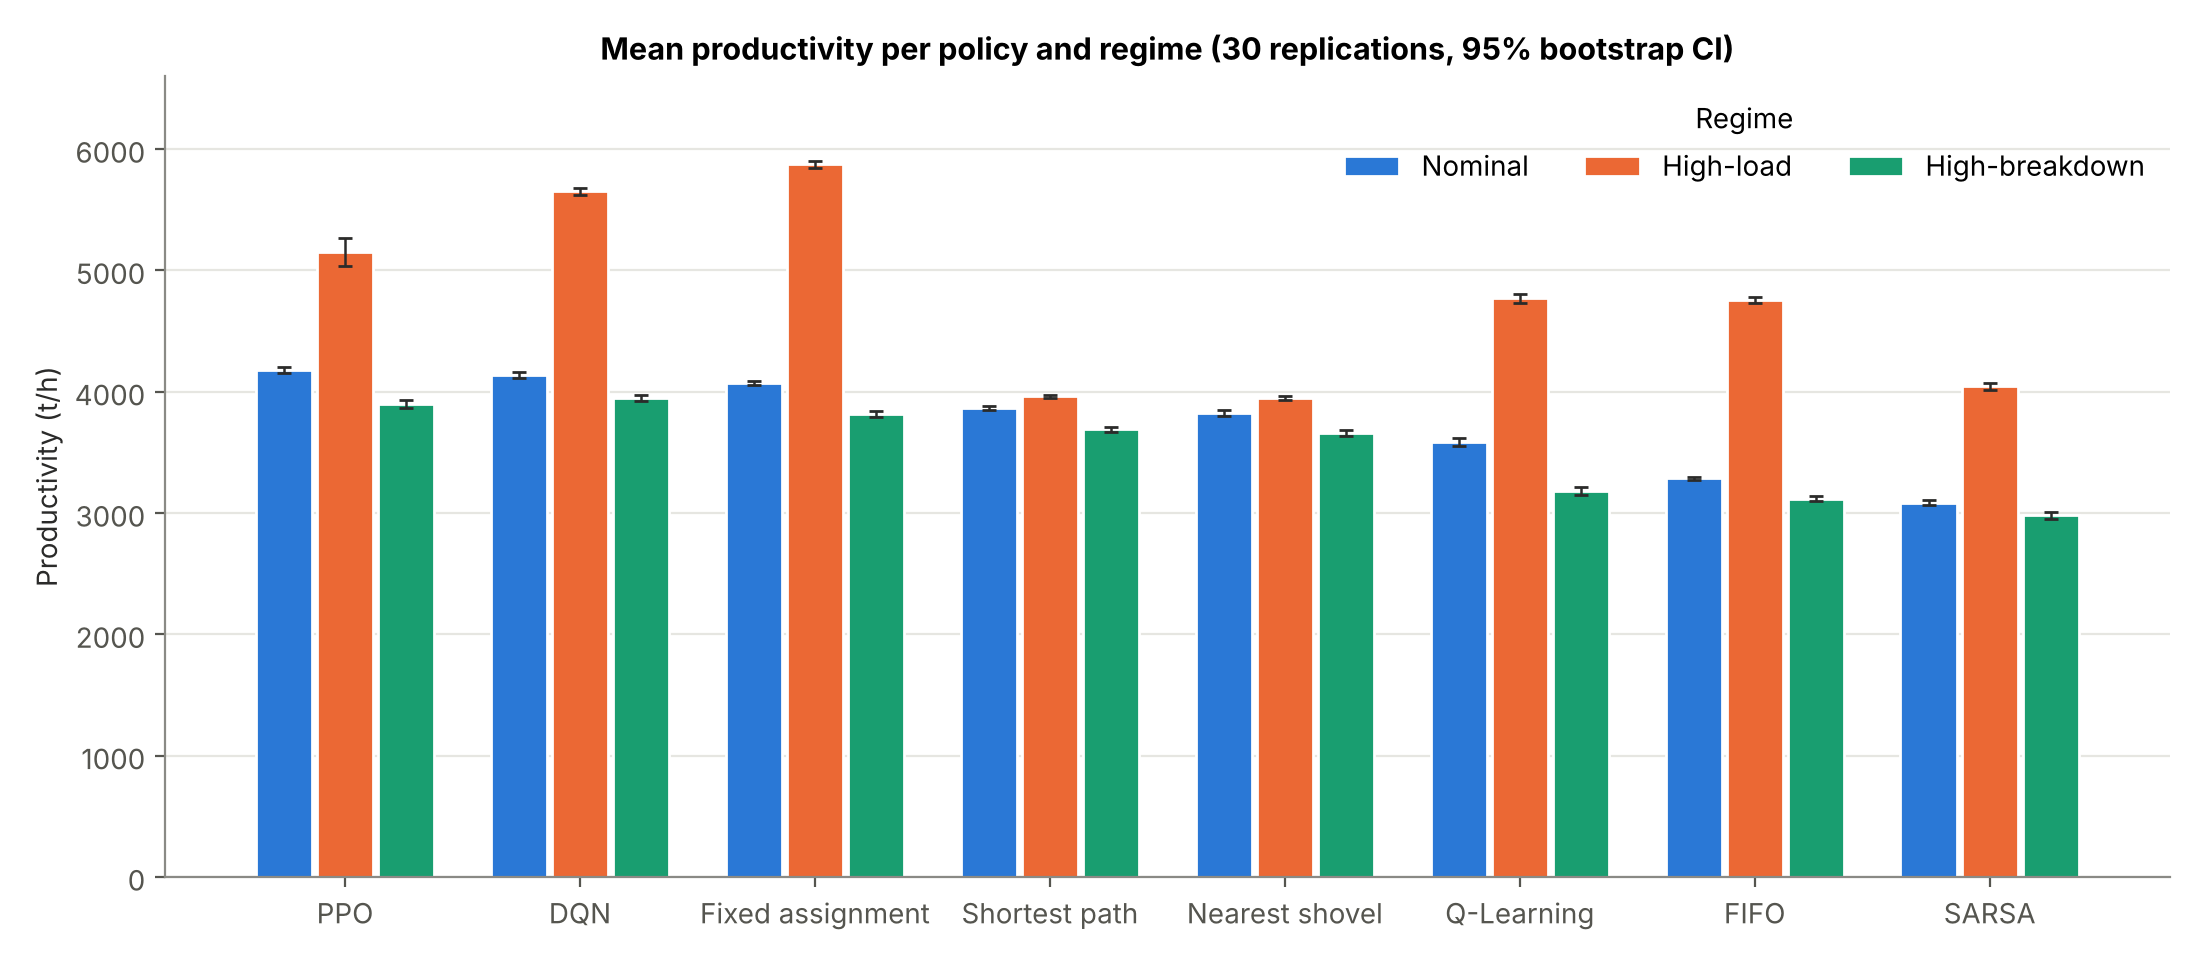
\includegraphics[width=0.92\textwidth]{figures/barplot_productivite_scenarios.png}
\caption{Productivité moyenne par politique et par régime. Les barres d'erreur indiquent les intervalles de confiance bootstrap à 95\,\% sur les 30 réplications uniques.}
\label{fig:productivity}
\end{figure}

\rev{M3}{\ifrevmarks\small Figure régénérée à partir des 30 réplications uniques.\fi}

Le \cref{tab:cycles_reward} rapporte le nombre de cycles terminés et la récompense cumulée. \rev{M18}{Le classement selon la récompense cumulée coïncide avec celui de la productivité en conditions nominales et en fortes pannes ; en forte charge, deux paires sont inversées (FIFO et Q-Learning, Pelle la plus proche et Plus court chemin).} La faible récompense de Pelle la plus proche et de Plus court chemin en forte charge (161,4 et 160,5) reflète à la fois un nombre de cycles plus faible et les pénalités d'attente et de déséquilibre entre pelles.

\begin{table}[H]
\centering
\caption{Nombre moyen de cycles terminés et récompense cumulée par politique et par régime, sur 30 réplications (N : nominal, FC : forte charge, FP : fortes pannes).}
\label{tab:cycles_reward}
\small
\setlength{\tabcolsep}{4pt}
\renewcommand{\arraystretch}{1.05}
\begin{tabularx}{\textwidth}{@{}l*{6}{>{\centering\arraybackslash}X}@{}}
\toprule
\multirow{2}{*}{\textbf{Politique}}
  & \multicolumn{3}{c}{\textbf{Cycles terminés}}
  & \multicolumn{3}{c}{\textbf{Récompense cumulée}} \\
\cmidrule(lr){2-4}\cmidrule(lr){5-7}
  & \textbf{N} & \textbf{FC} & \textbf{FP}
  & \textbf{N}   & \textbf{FC}   & \textbf{FP} \\
\midrule
FIFO              & 187,8 & 271,7 & 178,2 & 163,1 & 234,0 & 155,0 \\
Affectation fixe  & 232,7 & \textbf{335,6} & 218,2 & 210,7 & \textbf{301,3} & 197,7 \\
Pelle la plus proche & 218,6 & 225,6 & 209,2 & 193,0 & 161,4 & 185,7 \\
Plus court chemin & 221,0 & 226,4 & 211,0 & 194,7 & 160,5 & 187,0 \\
Q-Learning        & 204,9 & 272,5 & 181,8 & 178,9 & 230,6 & 155,6 \\
SARSA             & 176,3 & 231,1 & 170,3 & 147,3 & 179,7 & 143,2 \\
DQN               & 236,3 & 322,9 & \textbf{225,7} & 213,8 & 288,9 & \textbf{204,4} \\
PPO               & \textbf{238,7} & 294,2 & 222,8 & \textbf{216,6} & 253,0 & 201,5 \\
\bottomrule
\end{tabularx}
\end{table}

\subsection{Attente en file et immobilisation}
\label{sec:waiting}

\begin{revbloc}{M2, M17, m13, m14}
Le \cref{tab:waiting} distingue l'attente en file, qui mesure la congestion, du temps d'immobilisation total, qui y ajoute les pannes et l'attente volontaire. Les deux indicateurs sont exprimés en minutes par camion et par poste.

En conditions nominales, l'Affectation fixe présente l'attente en file la plus faible (22,2~min par camion et par poste, soit environ 1,1~min par cycle), suivie de PPO (24,5~min) et de FIFO (27,1~min). En forte charge, DQN présente l'attente en file la plus faible (31,6~min), devant l'Affectation fixe (35,6~min), PPO (38,2~min) et FIFO (39,6~min). Les deux règles fondées sur la distance atteignent environ 195 à 199~min de file, car toute la flotte attend devant la même pelle. Le temps d'immobilisation total de PPO en forte charge (99,3~min) provient pour plus de la moitié d'attentes volontaires : PPO choisit l'action ATTENDRE dans 87\,\% de ses décisions et cumule ainsi 54,7~min d'attente volontaire par camion, contre 38,2~min de file et 6,4~min de panne.

En fortes pannes, l'attente en file diminue pour la plupart des politiques par rapport aux conditions nominales, puisque moins de camions sont disponibles en même temps. L'augmentation du temps d'immobilisation total dans ce régime provient essentiellement des réparations, de 30 à 38~min par camion et par poste selon la politique, et non de la congestion.
\end{revbloc}

\begin{table}[H]
\centering
\caption{\rev{M2}{Attente en file et temps d'immobilisation total, en minutes par camion et par poste (moyenne $\pm$ écart-type de l'attente en file sur 30 réplications). Immobilisation totale = attente en file + panne + attente volontaire (action ATTENDRE).}}
\label{tab:waiting}
\footnotesize
\setlength{\tabcolsep}{4pt}
\begin{tabular}{lcc|cc|cc}
\toprule
 & \multicolumn{2}{c|}{\textbf{Nominal}} & \multicolumn{2}{c|}{\textbf{Forte charge}} & \multicolumn{2}{c}{\textbf{Fortes pannes}} \\
\textbf{Politique} & \textbf{File} & \textbf{Totale} & \textbf{File} & \textbf{Totale} & \textbf{File} & \textbf{Totale} \\
\midrule
FIFO                 & 27,1 $\pm$ 3,4 & 33,5 & 39,6 $\pm$ 3,2 & 45,2 & 23,4 $\pm$ 2,9 & 55,1 \\
Affectation fixe     & \textbf{22,2 $\pm$ 2,3} & \textbf{29,4} & 35,6 $\pm$ 3,2 & \textbf{43,2} & \textbf{19,5 $\pm$ 2,2} & 57,2 \\
Pelle la plus proche & 68,3 $\pm$ 6,9 & 75,1 & 194,6 $\pm$ 9,4 & 199,6 & 57,0 $\pm$ 5,8 & 93,8 \\
Plus court chemin    & 69,8 $\pm$ 6,5 & 76,6 & 199,3 $\pm$ 7,2 & 204,3 & 57,6 $\pm$ 5,5 & 94,7 \\
Q-Learning           & 52,6 $\pm$ 5,9 & 58,1 & 63,8 $\pm$ 3,7 & 69,3 & 56,6 $\pm$ 4,7 & 87,9 \\
SARSA                & 62,0 $\pm$ 6,0 & 68,2 & 114,2 $\pm$ 12,1 & 119,9 & 49,1 $\pm$ 5,5 & 81,8 \\
DQN                  & 29,0 $\pm$ 3,7 & 43,7 & \textbf{31,6 $\pm$ 2,5} & 47,8 & 29,7 $\pm$ 3,0 & 71,8 \\
PPO                  & 24,5 $\pm$ 2,7 & 33,5 & 38,2 $\pm$ 6,1 & 99,3 & 23,9 $\pm$ 3,5 & 69,9 \\
\bottomrule
\end{tabular}
\end{table}

\begin{figure}[H]
\centering
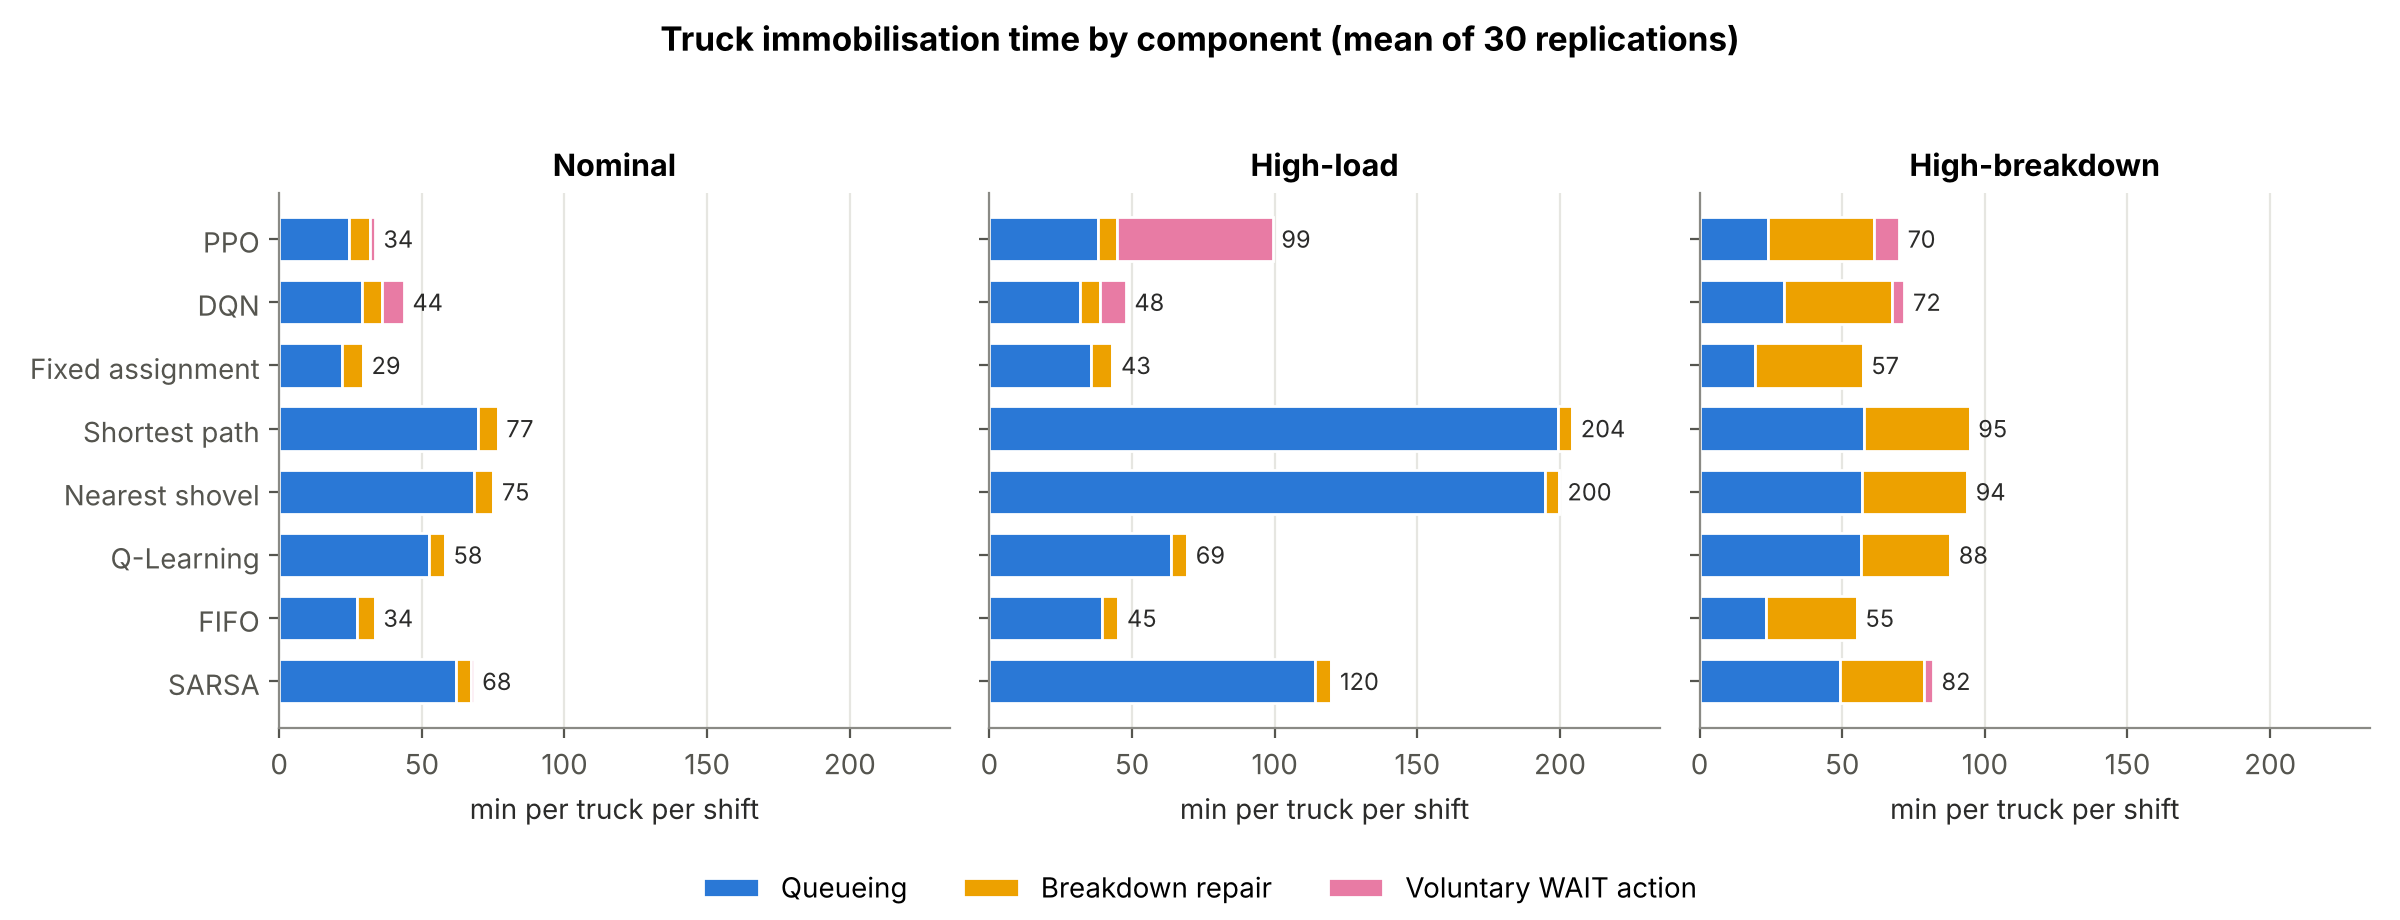
\includegraphics[width=\textwidth]{figures/wait_decomposition.png}
\caption{\rev{M2}{Décomposition du temps d'immobilisation des camions en attente en file, réparation après panne et attente volontaire (action ATTENDRE), en minutes par camion et par poste, pour les huit politiques et les trois régimes (moyennes sur 30 réplications).}}
\label{fig:waiting}
\end{figure}


\subsection{Comportement d'affectation des politiques}
\label{sec:behaviour}

\begin{revbloc}{M16, C3}
Le \cref{tab:behaviour} décrit, sur les 30 réplications, la répartition des cycles entre les trois pelles et la part des décisions consacrées à l'action ATTENDRE. Il explique plusieurs des écarts observés.

\begin{itemize}
  \item Pelle la plus proche et Plus court chemin réalisent 100\,\% de leurs cycles à la pelle 1, dans les trois régimes. La pelle 1 charge alors presque en permanence, tandis que les deux autres restent inutilisées. La congestion de ces deux règles n'est donc pas propre à la forte charge : elle existe dans tous les régimes et s'aggrave avec le nombre de camions qui attendent devant la même pelle.
  \item FIFO et l'Affectation fixe répartissent les cycles presque uniformément entre les pelles. L'Affectation fixe y parvient sans changer les camions de pelle, alors que FIFO déplace fréquemment les camions, ce qui allonge ses cycles (29,8~min contre 24,1~min en conditions nominales).
  \item En forte charge, PPO et DQN utilisent les trois pelles de façon équilibrée, mais choisissent très souvent d'attendre (87\,\% et 64\,\% des décisions). L'usage intensif de l'action ATTENDRE par PPO explique son temps d'immobilisation total élevé et sa grande variabilité dans ce régime.
  \item En fortes pannes, les deux agents profonds entraînés dans ce régime n'utilisent jamais la pelle 3, la plus éloignée, alors que les agents nominaux évalués sans réentraînement dans ce même régime utilisent les trois pelles (\cref{sec:robustness}).
\end{itemize}
\end{revbloc}

\begin{table}[H]
\centering
\caption{\rev{M16}{Répartition des cycles entre les pelles 1, 2 et 3 (\%) et part des décisions ATTENDRE (\%), moyennes sur 30 réplications.}}
\label{tab:behaviour}
\footnotesize
\setlength{\tabcolsep}{4pt}
\begin{tabular}{lcc|cc|cc}
\toprule
 & \multicolumn{2}{c|}{\textbf{Nominal}} & \multicolumn{2}{c|}{\textbf{Forte charge}} & \multicolumn{2}{c}{\textbf{Fortes pannes}} \\
\textbf{Politique} & \textbf{P1 / P2 / P3} & \textbf{Att.} & \textbf{P1 / P2 / P3} & \textbf{Att.} & \textbf{P1 / P2 / P3} & \textbf{Att.} \\
\midrule
FIFO                 & 36 / 34 / 30 & 0 & 36 / 34 / 30 & 0 & 35 / 34 / 32 & 0 \\
Affectation fixe     & 35 / 33 / 31 & 0 & 35 / 33 / 32 & 0 & 35 / 33 / 32 & 0 \\
Pelle la plus proche & 100 / 0 / 0 & 0 & 100 / 0 / 0 & 0 & 100 / 0 / 0 & 0 \\
Plus court chemin    & 100 / 0 / 0 & 0 & 100 / 0 / 0 & 0 & 100 / 0 / 0 & 0 \\
Q-Learning           & 17 / 52 / 31 & 0 & 28 / 30 / 41 & 1 & 42 / 37 / 21 & 0 \\
SARSA                & 9 / 50 / 41 & 5 & 5 / 60 / 34 & 1 & 5 / 29 / 66 & 10 \\
DQN                  & 63 / 16 / 21 & 35 & 26 / 41 / 33 & 64 & 59 / 41 / 0 & 31 \\
PPO                  & 43 / 41 / 16 & 10 & 34 / 34 / 32 & 87 & 63 / 37 / 0 & 48 \\
\bottomrule
\end{tabular}
\end{table}

\begin{figure}[H]
\centering
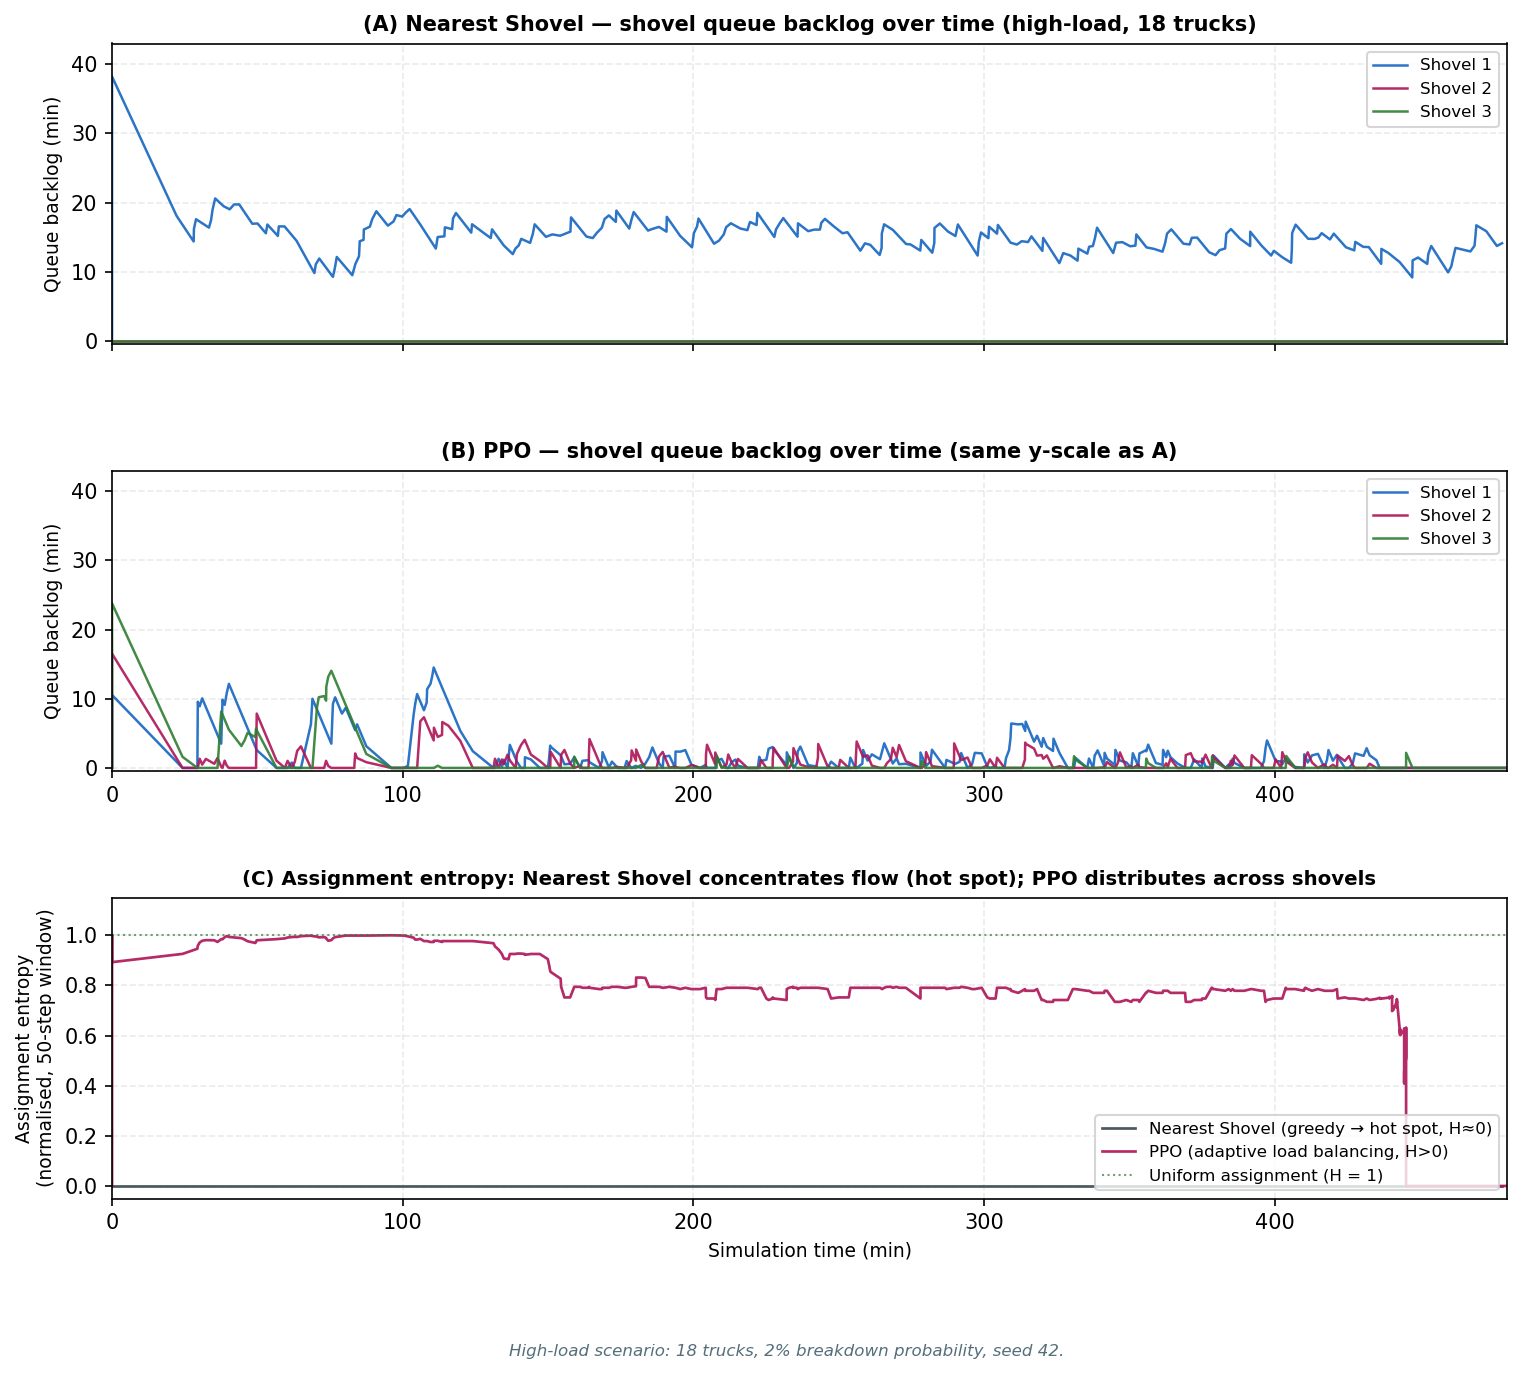
\includegraphics[width=0.96\textwidth]{figures/behavioral_analysis.png}
\caption{\rev{M16}{Illustration sur un seul épisode (forte charge, 18 camions, graine 42) : file résiduelle aux trois pelles pour Pelle la plus proche (A) et PPO (B), et entropie de Shannon normalisée de la répartition des affectations entre pelles sur une fenêtre glissante de 50 décisions (C), où 1 correspond à une répartition uniforme. Les valeurs agrégées sur 30 réplications figurent dans le \cref{tab:behaviour}.}}
\label{fig:behavioral}
\end{figure}

\afig{dans le panneau (C), retirer les mentions interprétatives de la légende (« adaptive load balancing », « greedy → hot spot ») : en forte charge, PPO choisit ATTENDRE dans 87\,\% de ses décisions, ce que la figure ne montre pas (M16).}

\subsection{Compromis entre productivité et attente en file}
\label{sec:pareto}

\begin{revbloc}{M19, H3}
Le \cref{tab:pareto} indique, pour chaque régime, les politiques non dominées au sens de Pareto lorsque l'on cherche à maximiser la productivité et à minimiser l'attente en file. Dans chaque régime, deux ou trois politiques forment le front : l'Affectation fixe et PPO en conditions nominales, l'Affectation fixe et DQN en forte charge, et DQN, PPO et l'Affectation fixe en fortes pannes. Le compromis entre les deux critères reste donc limité : les politiques les plus productives sont aussi, dans l'ensemble, celles qui attendent le moins, tandis que Pelle la plus proche et Plus court chemin sont dominées dans les trois régimes. Ces fronts sont définis à l'intérieur de chaque régime ; une comparaison entre régimes mélangerait des flottes de tailles différentes.
\end{revbloc}

\begin{table}[H]
\centering
\caption{\rev{M19}{Politiques non dominées au sens de Pareto dans chaque régime (productivité maximale, attente en file minimale).}}
\label{tab:pareto}
\small
\begin{tabularx}{\textwidth}{lX}
\toprule
\textbf{Régime} & \textbf{Front de Pareto} \\
\midrule
Nominal & Affectation fixe (4\,072~t/h ; 22,2~min), PPO (4\,177~t/h ; 24,5~min) \\
Forte charge & Affectation fixe (5\,874~t/h ; 35,6~min), DQN (5\,651~t/h ; 31,6~min) \\
Fortes pannes & Affectation fixe (3\,819~t/h ; 19,5~min), PPO (3\,900~t/h ; 23,9~min), DQN (3\,949~t/h ; 29,7~min) \\
\bottomrule
\end{tabularx}
\end{table}

\begin{figure}[H]
\centering
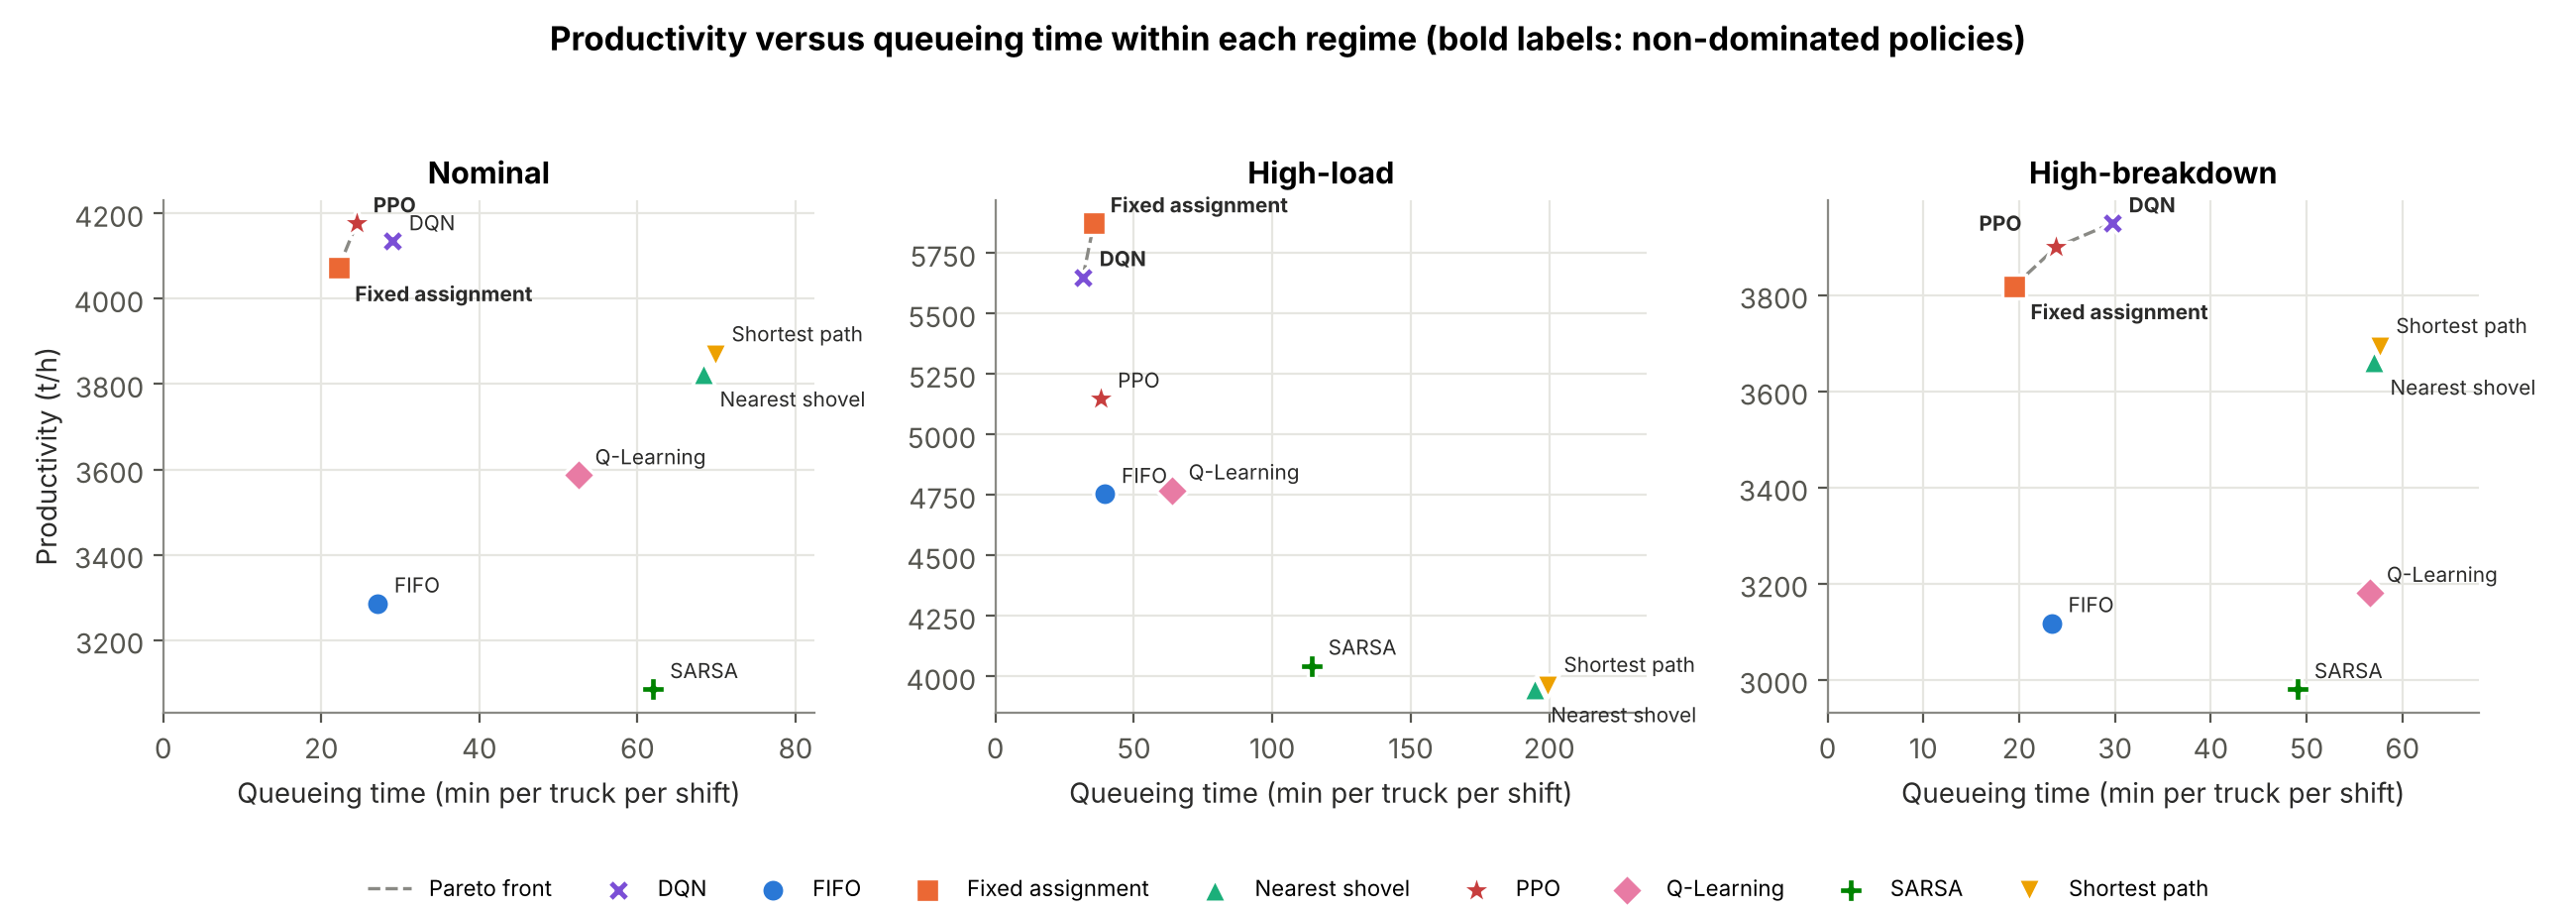
\includegraphics[width=0.88\textwidth]{figures/pareto_productivity_waiting.png}
\caption{\rev{M19}{Productivité en fonction de l'attente en file, dans chaque régime. Les politiques non dominées sont indiquées en gras et reliées par le front de Pareto en pointillés.}}
\label{fig:pareto}
\end{figure}


\subsection{Robustesse et transfert sans réentraînement}
\label{sec:robustness}

\begin{revbloc}{M1, M15, M17, QR3}
Les agents d'apprentissage comparés dans chaque régime ayant été entraînés dans ce régime, les ratios de robustesse du \cref{tab:robustness} comparent, pour ces agents, deux modèles différents : ils mesurent la performance obtenue après adaptation, et non la capacité d'un même agent à supporter un changement de régime. Cette seconde question est traitée par l'évaluation sans réentraînement du \cref{tab:transfer}.

L'indice d'augmentation de l'attente en file dans le régime $s$ est défini par :
\begin{equation}
\Delta_{\mathrm{file}}^{s} = \frac{W_{s} - W_{\mathrm{nominal}}}{W_{\mathrm{nominal}}} \times 100 ,
\label{eq:delta_wait}
\end{equation}
où $W$ est l'attente en file moyenne par camion et par poste.
\end{revbloc}

\begin{table}[H]
\centering
\caption{\rev{M15, M2, M17}{Robustesse par rapport aux conditions nominales. En forte charge (FC), le ratio est calculé sur la productivité par camion ; en fortes pannes (FP), sur la productivité. Les augmentations sont calculées sur l'attente en file, et, pour comparaison, sur le temps d'immobilisation total.}}
\label{tab:robustness}
\small
\setlength{\tabcolsep}{4pt}
\begin{tabular}{lcc|cc|c}
\toprule
 & \multicolumn{2}{c|}{\textbf{Ratio de robustesse}} & \multicolumn{2}{c|}{$\boldsymbol{\Delta_{\mathrm{file}}}$ \textbf{(\%)}} & \textbf{Immob. totale} \\
\textbf{Politique} & \textbf{FC (par camion)} & \textbf{FP} & \textbf{FC} & \textbf{FP} & \textbf{FC (\%)} \\
\midrule
FIFO                 & \textbf{0,965} & 0,949 & +45,9  & $-13{,}8$ & +35,0 \\
Affectation fixe     & 0,962 & 0,938 & +60,5  & $-12{,}2$ & +47,0 \\
Pelle la plus proche & 0,688 & 0,957 & +184,8 & $-16{,}6$ & +165,9 \\
Plus court chemin    & 0,683 & 0,955 & +185,4 & $-17{,}5$ & +166,7 \\
Q-Learning           & 0,887 & 0,887 & +21,4  & +7,8      & +19,4 \\
SARSA                & 0,874 & \textbf{0,966} & +84,2  & $-20{,}9$ & +75,9 \\
DQN                  & 0,911 & 0,955 & \textbf{+9,1} & +2,5 & \textbf{+9,3} \\
PPO                  & 0,822 & 0,934 & +56,0  & $-2{,}6$  & +196,4 \\
\bottomrule
\end{tabular}
\end{table}

\begin{revbloc}{M15, M17, M18}
En forte charge, une fois la productivité ramenée au nombre de camions, FIFO et l'Affectation fixe sont les politiques les plus robustes (ratios de 0,965 et 0,962), devant DQN (0,911) et PPO (0,822) ; les deux règles fondées sur la distance perdent près d'un tiers de leur productivité par camion. Les ratios supérieurs à 1 rapportés dans la version précédente reflétaient seulement l'ajout de 50\,\% de camions. Sur l'attente en file, DQN est la politique dont l'attente augmente le moins (+9,1\,\%), mais à partir d'un niveau nominal plus élevé que celui de l'Affectation fixe ; en valeur absolue, l'attente en file de DQN en forte charge (31,6~min) reste proche de celle de l'Affectation fixe (35,6~min). L'augmentation de 196\,\% du temps d'immobilisation total de PPO ne traduit pas une congestion, puisque son attente en file n'augmente que de 56\,\%, mais l'usage massif de l'action ATTENDRE.

En fortes pannes, toutes les politiques perdent entre 3 et 11\,\% de productivité. Les ratios les plus élevés de SARSA et des règles fondées sur la distance s'expliquent par leur productivité nominale déjà basse ; en valeur absolue, DQN, PPO et l'Affectation fixe restent les trois politiques les plus productives.
\end{revbloc}

\begin{table}[H]
\centering
\caption{\rev{M1, QR3}{Évaluation sans réentraînement : agents entraînés en conditions nominales et évalués dans un régime perturbé, comparés aux agents entraînés dans ce régime (productivité en t/h, moyenne $\pm$ écart-type sur 30 réplications ; $\Delta$ = transféré $-$ spécialisé, test de Wilcoxon apparié corrigé par Holm sur les six comparaisons). Référence : Affectation fixe, 3\,818,5~t/h en fortes pannes et 5\,873,6~t/h en forte charge.}}
\label{tab:transfer}
\small
\setlength{\tabcolsep}{4pt}
\begin{tabular}{llcccc}
\toprule
\textbf{Régime} & \textbf{Agent} & \textbf{Spécialisé} & \textbf{Nominal transféré} & \textbf{$\Delta$ (t/h)} & \textbf{$p$ (Holm)} \\
\midrule
Fortes pannes & PPO        & 3\,899,6 $\pm$ 85  & 3\,926,4 $\pm$ 62  & +26,8   & 0,062 \\
              & DQN        & 3\,949,2 $\pm$ 72  & 3\,882,1 $\pm$ 69  & $-67{,}1$ & $<0{,}001$ \\
              & Q-Learning & 3\,180,9 $\pm$ 92  & 3\,410,8 $\pm$ 127 & +229,8  & $<0{,}001$ \\
              & SARSA      & 2\,980,8 $\pm$ 78  & 2\,923,1 $\pm$ 59  & $-57{,}8$ & 0,005 \\
Forte charge  & Q-Learning & 4\,769,3 $\pm$ 102 & 4\,702,3 $\pm$ 195 & $-67{,}1$ & 0,18 \\
              & SARSA      & 4\,044,8 $\pm$ 76  & 4\,136,4 $\pm$ 87  & +91,6   & 0,002 \\
\bottomrule
\end{tabular}
\end{table}

\begin{revbloc}{M1, QR3}
Le \cref{tab:transfer} montre que réentraîner les agents dans le régime perturbé n'apporte qu'un gain limité, voire aucun. En fortes pannes, l'agent PPO nominal transféré obtient une productivité au moins égale à celle de l'agent spécialisé (+26,8~t/h, différence non significative après correction), et l'agent DQN nominal transféré perd 67,1~t/h par rapport à l'agent spécialisé. Les deux agents profonds transférés restent nettement plus productifs que l'Affectation fixe (+107,9 et +63,6~t/h, $p<0{,}001$). Leurs ratios de robustesse sont de 0,940 pour PPO et 0,939 pour DQN, contre 0,938 pour l'Affectation fixe. L'agent PPO transféré utilise les trois pelles et n'attend presque jamais (1\,\% des décisions), alors que l'agent spécialisé attend dans 48\,\% de ses décisions. Pour les agents tabulaires, les écarts entre agent transféré et agent spécialisé sont de signes variables, ce qui est cohérent avec la non-convergence de leur entraînement (\cref{sec:convergence}). Ces résultats ont été obtenus en rejouant les agents nominaux, sans modification, dans le simulateur de l'étude.
\end{revbloc}

\aexp{reproduire le \cref{tab:transfer} avec la fonction \texttt{run\_benchmark} et l'argument \texttt{model\_scenario="nominal"} pour le régime de fortes pannes, et prévoir une observation de taille fixe (remplissage jusqu'à 18 camions avec masque, ou variables agrégées par pelle) pour évaluer PPO et DQN sans réentraînement en forte charge (M1).}

\begin{figure}[H]
\centering
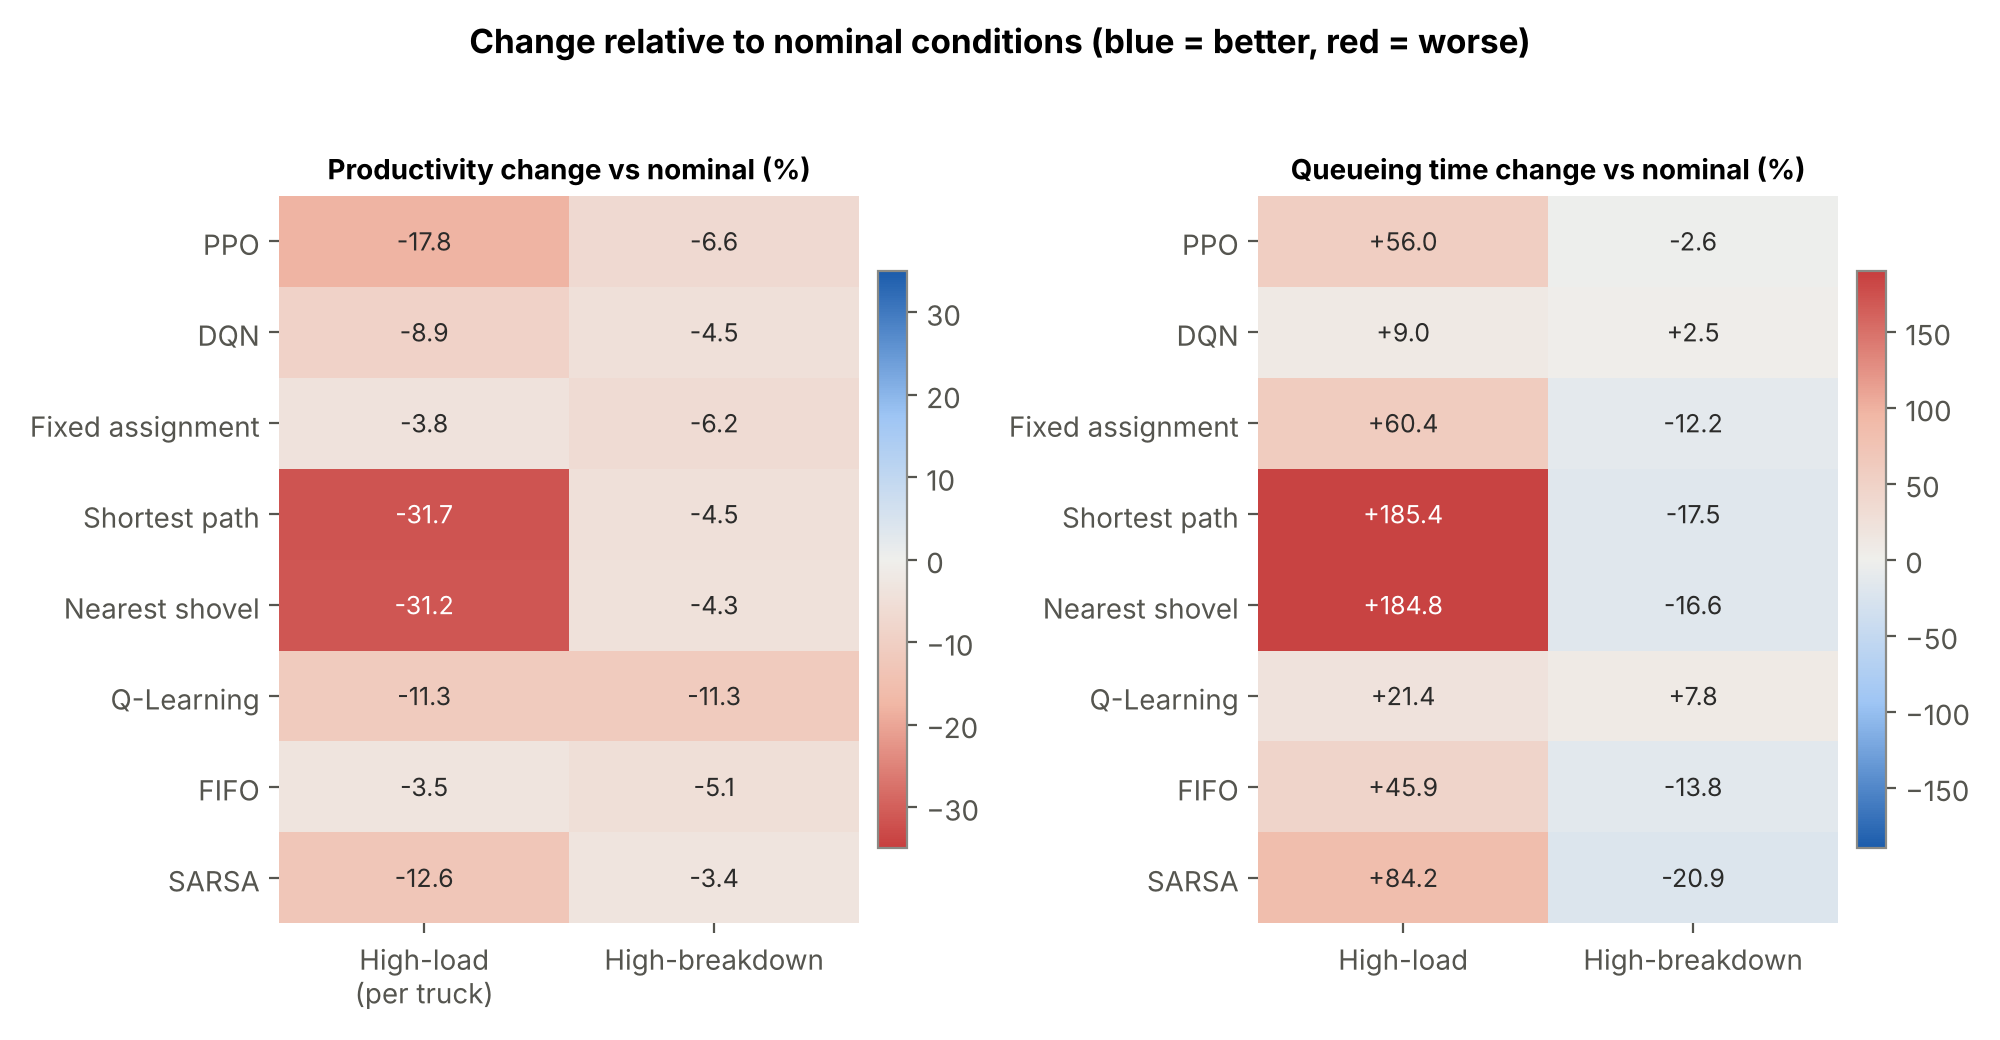
\includegraphics[width=0.9\textwidth]{figures/robustness_heatmap.png}
\caption{\rev{M15, M2}{Variation par rapport aux conditions nominales, en \%. Gauche : productivité (par camion en forte charge). Droite : attente en file. Le bleu indique une amélioration et le rouge une dégradation.}}
\label{fig:heatmap}
\end{figure}


\subsection{Significativité statistique}
\label{sec:stats}

\begin{revbloc}{M3, M4, M5, M6}
Le test de Friedman met en évidence un effet de la politique sur la productivité dans chacun des trois régimes ($\chi^2(7) = 207{,}6$ en conditions nominales, 200,7 en forte charge et 202,6 en fortes pannes ; $p<0{,}001$ dans les trois cas). Le modèle linéaire de la productivité par camion révèle une interaction significative entre politique et régime ($F(14, 609) = 430{,}4$, $p<0{,}001$, $\eta^2_p = 0{,}91$) : l'effet de la politique dépend du régime, ce qui constitue la preuve principale de l'hypothèse H2.

Le \cref{tab:stats} rapporte les comparaisons par paires entre les deux agents profonds et l'Affectation fixe, meilleure heuristique dans les trois régimes, ainsi qu'entre PPO et DQN. Toutes ces différences sont significatives après correction de Holm. En particulier, l'avantage de l'Affectation fixe sur DQN en forte charge, celui de PPO sur l'Affectation fixe en fortes pannes et celui de DQN sur PPO en fortes pannes, que le test de Dunn utilisé dans la version précédente ne détectait pas, apparaissent clairement avec le test apparié. Ces comparaisons portent toutefois sur un modèle entraîné par algorithme : elles opposent deux agents entraînés, et non deux algorithmes (\cref{sec:limitations}).
\end{revbloc}

\begin{table}[H]
\centering
\caption{\rev{M3, M4, M6}{Comparaisons par paires de la productivité : différence moyenne appariée (t/h) avec intervalle de confiance bootstrap à 95\,\%, $d$ de Cohen et valeur $p$ du test de Wilcoxon apparié, bilatéral, corrigée par Holm sur les trois comparaisons de chaque régime.}}
\label{tab:stats}
\footnotesize
\setlength{\tabcolsep}{4pt}
\begin{tabular}{llccc}
\toprule
\textbf{Régime} & \textbf{Comparaison} & \textbf{Différence [IC 95\,\%]} & \textbf{$d$} & \textbf{$p$ (Holm)} \\
\midrule
Nominal       & PPO $-$ Aff. fixe & +105,0 [88,1 ; 120,8]   & 1,93 & $<0{,}001$ \\
              & DQN $-$ Aff. fixe & +63,0 [45,5 ; 81,1]     & 1,10 & $<0{,}001$ \\
              & PPO $-$ DQN       & +42,0 [28,6 ; 56,6]     & 0,64 & $<0{,}001$ \\
Forte charge  & PPO $-$ Aff. fixe & $-724{,}5$ [$-836{,}5$ ; $-606{,}1$] & $-3{,}07$ & $<0{,}001$ \\
              & DQN $-$ Aff. fixe & $-222{,}2$ [$-242{,}7$ ; $-200{,}7$] & $-2{,}98$ & $<0{,}001$ \\
              & PPO $-$ DQN       & $-502{,}2$ [$-617{,}8$ ; $-380{,}9$] & $-2{,}13$ & $<0{,}001$ \\
Fortes pannes & PPO $-$ Aff. fixe & +81,1 [54,3 ; 106,2]    & 1,06 & $<0{,}001$ \\
              & DQN $-$ Aff. fixe & +130,7 [112,0 ; 148,8]  & 1,88 & $<0{,}001$ \\
              & PPO $-$ DQN       & $-49{,}6$ [$-74{,}1$ ; $-26{,}3$] & $-0{,}63$ & $<0{,}001$ \\
\bottomrule
\end{tabular}
\end{table}

\subsection{Variabilité entre réplications d'évaluation}
\label{sec:stability}

\begin{revbloc}{M7}
Le coefficient de variation de la productivité sur les 30 réplications mesure la variabilité due à l'environnement pour un agent entraîné donné. Plus court chemin présente le coefficient moyen le plus faible sur les trois régimes (1,25\,\%), suivi de l'Affectation fixe (1,37\,\%), de FIFO (1,52\,\%) et de Pelle la plus proche (1,53\,\%). DQN est l'agent d'apprentissage le moins variable (1,59\,\%). PPO présente la variabilité la plus élevée (3,34\,\%), due presque entièrement à la forte charge (6,31\,\%, écart-type de 325~t/h), régime dans lequel il recourt massivement à l'action ATTENDRE. Les agents tabulaires présentent également une variabilité élevée (Q-Learning : 2,59\,\%, SARSA : 2,18\,\%). Cette analyse ne renseigne pas sur la variabilité due à l'entraînement, qui exigerait plusieurs graines d'entraînement par agent.
\end{revbloc}

\subsection{Convergence}
\label{sec:convergence}

\begin{revbloc}{M7, m24}
Les courbes d'entraînement des quatre agents sont présentées dans la \cref{fig:convergence}. Chaque courbe correspond à un seul entraînement, lissé par une moyenne mobile ; aucune bande de confiance ne peut donc être tracée.

\begin{itemize}
  \item \textbf{Agents profonds :} PPO et DQN atteignent un plateau dans leur budget de 2~millions de pas. La productivité de PPO augmente de façon monotone jusqu'à un plateau d'environ 4\,000 à 4\,200~t/h ; DQN présente des oscillations initiales plus importantes, liées à son exploration, avant de se stabiliser à un niveau similaire.
  \item \textbf{Agents tabulaires :} Q-Learning stagne pendant environ 12\,000 épisodes, puis s'améliore régulièrement jusqu'à la fin du budget sans atteindre de plateau ; sa performance rapportée doit donc être lue comme une borne inférieure. SARSA ne montre pas d'amélioration mesurable sur le même budget. Ces résultats indiquent que la représentation réduite à six variables discrétisées ne suffit pas, dans le budget retenu, à apprendre une politique compétitive.
\end{itemize}

Les agents profonds et tabulaires sont tracés sur des panneaux séparés, car ils sont enregistrés sur des grandeurs différentes : la productivité pour les agents profonds, la récompense cumulée par épisode pour les agents tabulaires.
\end{revbloc}

\begin{figure}[H]
\centering
\begin{subfigure}[b]{0.49\textwidth}
  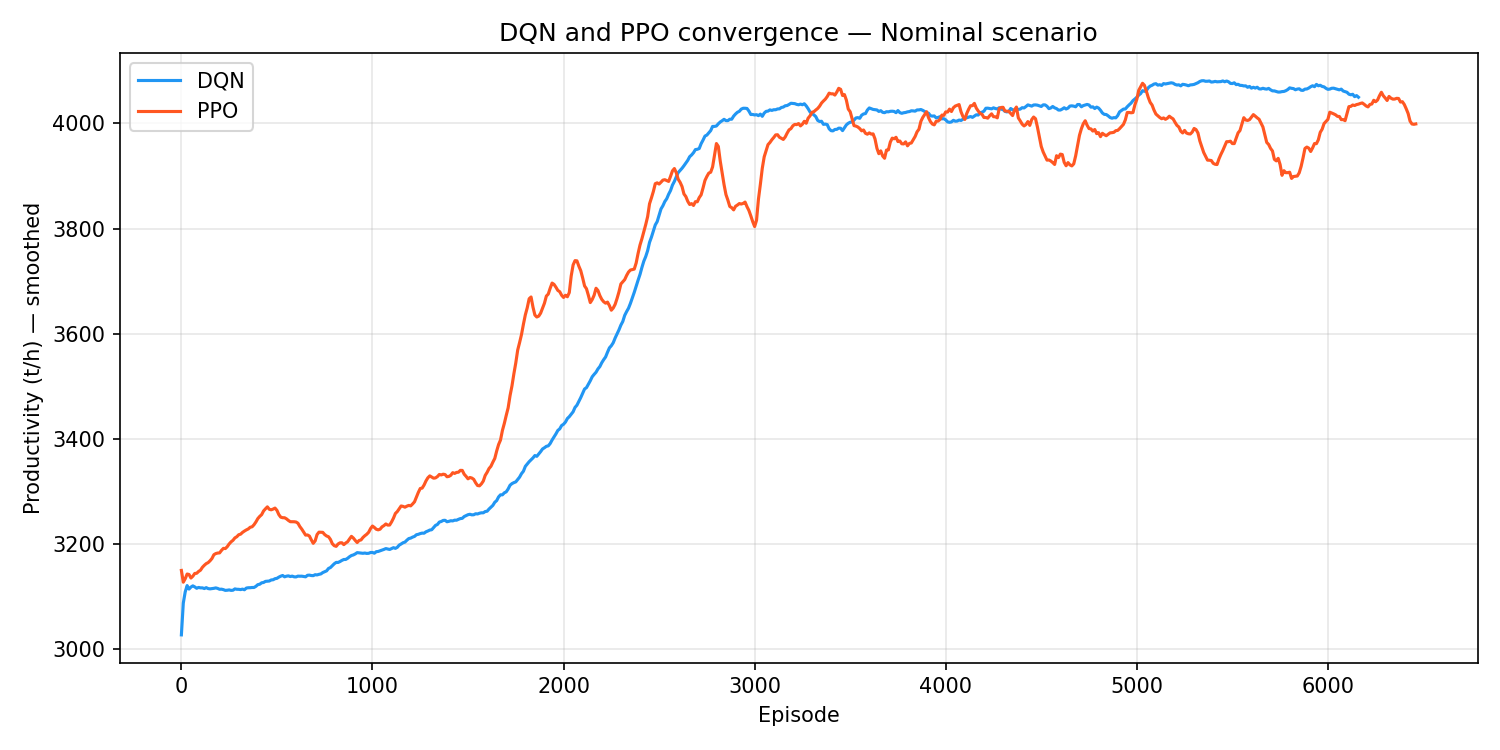
\includegraphics[width=\textwidth]{figures/learning_curves_deeprl_nominal.png}
  \caption{Agents profonds (DQN, PPO), régime nominal}
\end{subfigure}
\hfill
\begin{subfigure}[b]{0.49\textwidth}
  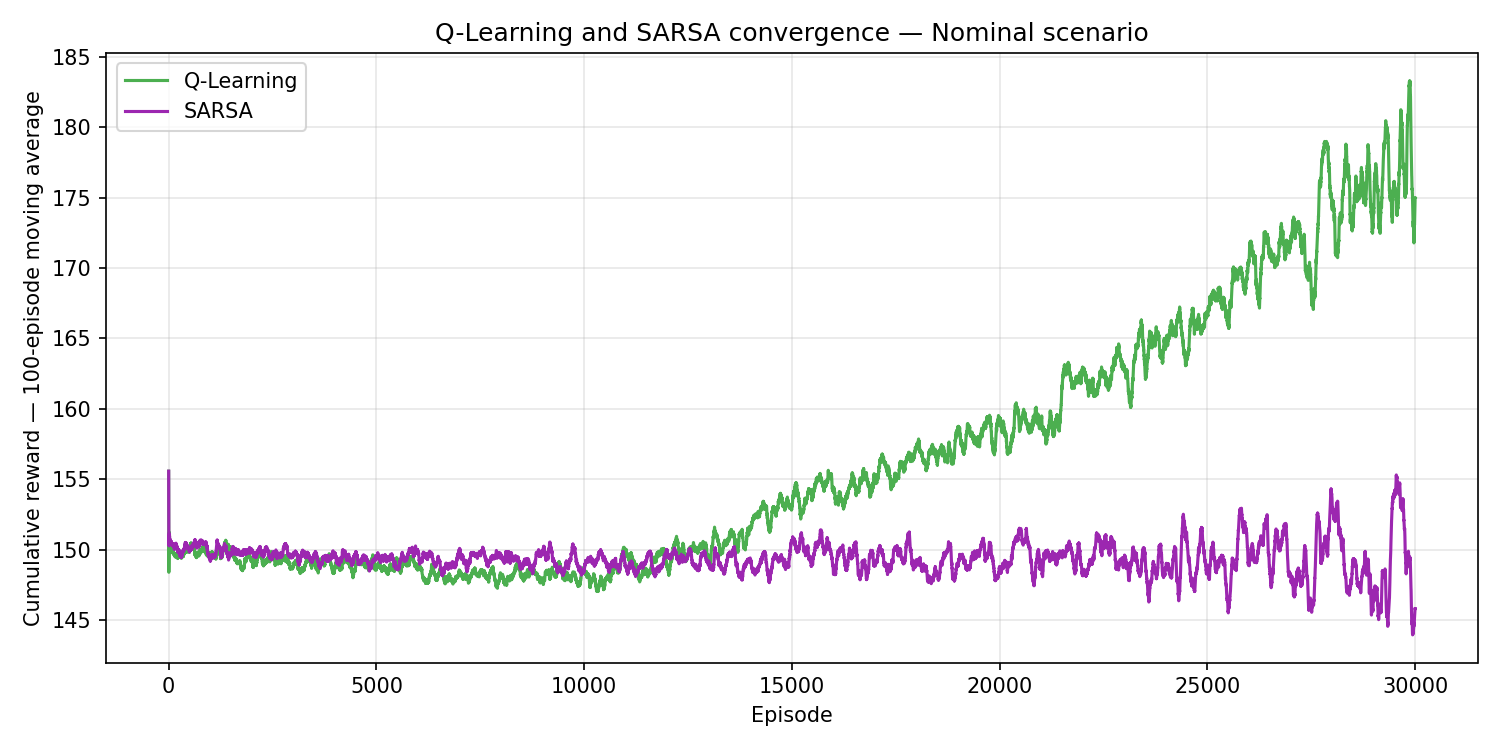
\includegraphics[width=\textwidth]{figures/learning_curves_nominal.png}
  \caption{Agents tabulaires (Q-Learning, SARSA), régime nominal}
\end{subfigure}
\caption{Courbes d'entraînement dans le régime nominal, un seul entraînement par agent. Gauche : productivité des agents profonds. Droite : récompense cumulée par épisode des agents tabulaires, moyenne mobile sur 100 épisodes.}
\label{fig:convergence}
\end{figure}

\aexp{tracer les courbes de convergence en moyenne $\pm$ intervalle sur 5 graines d'entraînement (M7, Dir. plan).}

\subsection{Étude d'ablation}
\label{sec:ablation}

\begin{revbloc}{M13, A}
L'étude d'ablation porte sur le poids de la pénalité d'attente $w_4$, les autres poids étant constants. Pour chaque valeur de $w_4$, PPO et DQN ont été entraînés une fois, avec la graine 42 ; la moyenne et l'écart-type sont calculés sur les 30 réplications d'évaluation de chaque modèle. L'entraînement étant déterministe, le modèle obtenu pour $w_4 = 0{,}3$ est identique à celui des résultats principaux.

Pour PPO, la relation entre $w_4$ et la performance n'est pas monotone : la productivité vaut 4\,161~t/h pour $w_4 = 0$, chute à 3\,932~t/h pour $w_4 = 0{,}1$, remonte à 4\,177~t/h pour $w_4 = 0{,}3$ et chute à 3\,684~t/h pour $w_4 = 0{,}5$, avec une variabilité nettement plus grande (écart-type de 158~t/h). Pour DQN, la productivité diminue légèrement et régulièrement avec $w_4$ (de 4\,174 à 4\,092~t/h), tandis que le temps d'immobilisation est le plus faible pour $w_4 = 0{,}5$. Comme chaque configuration repose sur un seul entraînement, la dégradation observée pour PPO à $w_4 = 0{,}1$ est compatible avec un compromis de récompense défavorable, mais plusieurs entraînements indépendants seraient nécessaires pour la distinguer de la variabilité de l'entraînement. Le choix $w_4 = 0{,}3$ donne la meilleure productivité pour PPO, mais pas pour DQN, qui obtient sa meilleure productivité sans pénalité d'attente.
\end{revbloc}

\begin{table}[H]
\centering
\caption{\rev{M13}{Étude d'ablation sur le poids de la pénalité d'attente $w_4$, régime nominal. Productivité (t/h) et temps d'immobilisation total (min par camion et par poste), moyenne $\pm$ écart-type sur 30 réplications d'un seul modèle entraîné par configuration.}}
\label{tab:ablation}
\small
\begin{tabular}{lcccc}
\toprule
 & \multicolumn{2}{c}{\textbf{PPO}} & \multicolumn{2}{c}{\textbf{DQN}} \\
\cmidrule(lr){2-3}\cmidrule(lr){4-5}
\textbf{$w_4$} & \textbf{Productivité} & \textbf{Immobilisation} & \textbf{Productivité} & \textbf{Immobilisation} \\
\midrule
0,0  & 4\,160,9 $\pm$ 64 & 41,5 $\pm$ 4,8 & \textbf{4\,174,3 $\pm$ 55} & 44,2 $\pm$ 5,1 \\
0,1  & 3\,931,7 $\pm$ 52 & 74,8 $\pm$ 4,6 & 4\,156,3 $\pm$ 63 & 39,2 $\pm$ 4,3 \\
0,3 (réf.) & \textbf{4\,176,7 $\pm$ 64} & \textbf{33,5 $\pm$ 4,8} & 4\,134,7 $\pm$ 68 & 43,7 $\pm$ 5,2 \\
0,5  & 3\,683,8 $\pm$ 158 & 79,3 $\pm$ 20,3 & 4\,091,5 $\pm$ 61 & \textbf{31,0 $\pm$ 4,2} \\
\bottomrule
\end{tabular}
\end{table}

\aexp{entraîner 3 à 5 graines par valeur de $w_4$ pour distinguer l'effet de la récompense de la variabilité de l'entraînement (M13).}

\paragraph{Sensibilité aux hyperparamètres.}
\begin{revbloc}{M12}
La configuration de PPO suit les réglages usuels de l'algorithme \cite{JohnSchulman2017} et les valeurs par défaut de Stable-Baselines3. Des essais préliminaires sur le coefficient d'entropie ($c_H \in \{0\,;\,0{,}01\,;\,0{,}02\,;\,0{,}05\}$) ont conduit à retenir $c_H = 0{,}02$. DQN a été utilisé avec ses valeurs par défaut, à l'exception de la taille du tampon et du calendrier d'exploration indiqués dans le \cref{tab:hyper}. L'effort de réglage n'a donc pas été le même pour les deux agents profonds, ce qui constitue une limite de la comparaison entre PPO et DQN.
\end{revbloc}

\adir{les essais préliminaires sur $c_H$ ne figurent dans aucun script du projet : fournir un tableau chiffré (valeurs testées, régime, critère, graines distinctes de l'évaluation) ou supprimer cette mention (M12).}


% ============================================================================
% Section 8 : Discussion
% ============================================================================
\section{Discussion}
\label{sec:discussion}

Cette section interprète les résultats au regard des questions de recherche, discute les implications pour l'exploitation et la durabilité, puis les limites de l'étude.

\subsection{Réponses aux questions de recherche}

\begin{revbloc}{M18, M23}
\textbf{QR1.} Aucune politique n'atteint la productivité la plus élevée dans les trois régimes : PPO est en tête en conditions nominales, l'Affectation fixe en forte charge et DQN en fortes pannes. Le classement dépend donc de l'interaction entre la logique de dispatching et le régime, et non de la seule famille d'algorithmes.

\textbf{QR2.} Dans chaque régime, productivité et attente en file évoluent globalement dans le même sens : les politiques les plus productives sont aussi celles qui attendent le moins, et le front de Pareto ne compte que deux ou trois politiques. Le type de logique de dispatching compte davantage que la distinction entre apprentissage et règles : les deux règles qui ignorent les files concentrent la flotte sur une pelle et sont dominées partout, tandis que l'Affectation fixe, qui répartit les camions de façon équilibrée et stable, reste compétitive dans les trois régimes.

\textbf{QR3.} En fortes pannes, les agents profonds entraînés en conditions nominales conservent, sans réentraînement, une productivité proche de celle des agents entraînés dans ce régime et supérieure à celle de l'Affectation fixe. Dans cette étude, la robustesse aux pannes de camions ne dépend donc pas d'un réentraînement spécifique. La question reste ouverte pour la forte charge, où la représentation de l'état empêche le transfert des agents profonds.

\textbf{QR4.} Le classement selon la consommation spécifique ne suit pas exactement celui de la productivité (\cref{sec:sustainability}) : DQN consomme le moins par tonne en conditions nominales et en fortes pannes, sans être le plus productif en conditions nominales.
\end{revbloc}

Le \cref{tab:hypotheses} résume le statut des trois hypothèses.

\begin{table}[H]
\caption{\rev{M23, M3}{Validation des hypothèses de recherche.}}
\label{tab:hypotheses}
\footnotesize\setlength{\tabcolsep}{4pt}
\begin{tabularx}{\textwidth}{@{}lXXl@{}}
\toprule
\textbf{Hyp.} & \textbf{Énoncé} & \textbf{Éléments clés} & \textbf{Verdict} \\
\midrule
H1 & En conditions nominales, les agents profonds dépassent la meilleure heuristique en productivité. & PPO : +105~t/h (+2,6\,\%) et DQN : +63~t/h (+1,6\,\%) par rapport à l'Affectation fixe, $p<0{,}001$ (\cref{tab:stats}). Résultat obtenu avec un seul entraînement par agent. & \textbf{Validée} \\[4pt]
H2 & Aucune politique ne domine dans les trois régimes. & Meilleure politique différente dans chaque régime ; interaction entre politique et régime significative ($F(14,609)=430{,}4$, $p<0{,}001$). & \textbf{Validée} \\[4pt]
H3 & Une productivité élevée ne s'accompagne pas nécessairement d'une faible attente en file. & Compromis limité entre l'Affectation fixe et PPO en conditions nominales, entre l'Affectation fixe et DQN en forte charge ; dans l'ensemble, productivité et faible attente vont de pair, et les règles fondées sur la distance sont mauvaises sur les deux critères. & Partiellement validée \\
\bottomrule
\end{tabularx}
\end{table}

\subsection{Interprétation}

\begin{revbloc}{M14, M16, M18, M27}
\begin{itemize}
  \item \textbf{L'équilibre de la répartition explique une grande part des écarts.} Les trois politiques les plus productives répartissent les cycles entre plusieurs pelles, alors que les deux règles fondées sur la distance les concentrent sur une seule. L'Affectation fixe, qui fige une répartition équilibrée, est ainsi très difficile à battre lorsque la flotte augmente, car elle évite à la fois la congestion et les déplacements inutiles entre pelles.
  \item \textbf{PPO et DQN.} En conditions nominales, PPO devance DQN de 42~t/h ; en fortes pannes, DQN devance PPO de 50~t/h. Ces écarts opposent deux modèles entraînés une fois chacun, et non deux algorithmes. Une explication possible de l'avantage de DQN en fortes pannes est la réutilisation, par son tampon de rejeu, des transitions impliquant des pannes ; aucune expérience de cette étude ne permet toutefois de l'établir, et le transfert sans réentraînement montre que l'agent PPO nominal fait aussi bien que l'agent PPO spécialisé dans ce régime.
  \item \textbf{L'action ATTENDRE.} En forte charge, PPO a appris à faire patienter les camions dans la grande majorité de ses décisions. Cette stratégie limite peu l'attente en file mais réduit la productivité par camion et rend la performance très variable d'une réplication à l'autre. Elle montre que la conception de l'espace d'actions et de la récompense, et pas seulement l'algorithme, détermine le comportement appris.
  \item \textbf{Un problème multi-objectif et stochastique.} Le dispatching doit être évalué sur plusieurs critères et plusieurs régimes : une évaluation limitée aux conditions nominales aurait désigné PPO comme la politique à déployer, alors qu'il est troisième en forte charge.
\end{itemize}
\end{revbloc}

\subsection{Implications pour l'exploitation}

\begin{revbloc}{M27}
Les résultats portent sur la performance relative des politiques dans l'environnement simulé proposé, et leur transposition à un site réel exigerait une calibration et une validation préalables. Sous cette réserve, trois enseignements se dégagent. Premièrement, un agent d'apprentissage devrait d'abord être utilisé comme aide à la décision, ses recommandations étant validées par un répartiteur, plutôt que comme un remplacement des systèmes de gestion de flotte. Deuxièmement, une politique candidate devrait être évaluée sur plusieurs régimes contrastés, à l'aide d'un jumeau numérique, avant tout déploiement. Troisièmement, une règle simple et bien équilibrée, telle que l'Affectation fixe, constitue une référence exigeante qu'une politique apprise doit dépasser dans tous les régimes pertinents.

Le passage à de grandes flottes de 50 à 200 camions et l'exploitation des données de télémétrie que produisent ces flottes constituent une perspective importante. La représentation de l'état utilisée ici, dont la taille croît avec le nombre de camions, ne s'y prête pas ; des représentations indépendantes de la taille de la flotte, telles que des réseaux de neurones sur graphe, et des formulations multi-agents \cite{Zhao2025} pourraient le permettre. Un préentraînement sur des historiques de dispatching suivi d'un ajustement en simulation pourrait réduire l'écart entre simulation et réalité ; ces pistes restent à évaluer.
\end{revbloc}

\subsection{Durabilité}
\label{sec:sustainability}

Le \cref{tab:efficiency} rapporte l'utilisation des camions et des pelles, et le \cref{tab:fuel} la consommation spécifique de carburant.

\begin{table}[H]
\centering
\caption{\rev{M2, m18}{Utilisation des camions (temps d'activité dans le poste) et des pelles (temps de chargement), en \%, moyennes sur 30 réplications.}}
\label{tab:efficiency}
\footnotesize\setlength{\tabcolsep}{4pt}
\begin{tabular}{lccc|ccc}
\toprule
 & \multicolumn{3}{c|}{\textbf{Utilisation des camions (\%)}} & \multicolumn{3}{c}{\textbf{Utilisation des pelles (\%)}} \\
\textbf{Politique} & \textbf{N} & \textbf{FC} & \textbf{FP} & \textbf{N} & \textbf{FC} & \textbf{FP} \\
\midrule
FIFO                 & 93,0 & 90,6 & \textbf{88,5} & 27,9 & 40,3 & 26,4 \\
Affectation fixe     & \textbf{93,9} & \textbf{91,0} & 88,1 & 34,0 & \textbf{49,2} & 32,0 \\
Pelle la plus proche & 84,4 & 58,4 & 80,5 & 32,0 & 33,8 & 30,8 \\
Plus court chemin    & 84,0 & 57,4 & 80,3 & 32,4 & 34,0 & 31,0 \\
Q-Learning           & 87,9 & 85,6 & 81,7 & 30,2 & 40,4 & 26,9 \\
SARSA                & 85,8 & 75,0 & 83,0 & 26,2 & 34,6 & 25,4 \\
DQN                  & 91,1 & 90,1 & 85,1 & 33,4 & 45,6 & \textbf{32,1} \\
PPO                  & 93,1 & 79,4 & 85,5 & \textbf{34,4} & 41,0 & 31,4 \\
\bottomrule
\end{tabular}
\end{table}

\begin{table}[H]
\centering
\caption{\rev{M20, m16}{Consommation spécifique de carburant (L/t), moyenne $\pm$ écart-type sur 30 réplications.}}
\label{tab:fuel}
\footnotesize\setlength{\tabcolsep}{4pt}
\begin{tabular}{lccc}
\toprule
\textbf{Politique} & \textbf{N} & \textbf{FC} & \textbf{FP} \\
\midrule
FIFO                 & $0{,}0534\pm0{,}0006$ & $0{,}0546\pm0{,}0004$ & $0{,}0555\pm0{,}0007$ \\
Affectation fixe     & $0{,}0431\pm0{,}0003$ & $\mathbf{0{,}0444\pm0{,}0004}$ & $0{,}0453\pm0{,}0006$ \\
Pelle la plus proche & $0{,}0430\pm0{,}0004$ & $0{,}0582\pm0{,}0006$ & $0{,}0445\pm0{,}0005$ \\
Plus court chemin    & $0{,}0432\pm0{,}0004$ & $0{,}0588\pm0{,}0005$ & $0{,}0447\pm0{,}0006$ \\
Q-Learning           & $0{,}0482\pm0{,}0012$ & $0{,}0537\pm0{,}0010$ & $0{,}0534\pm0{,}0014$ \\
SARSA                & $0{,}0555\pm0{,}0009$ & $0{,}0612\pm0{,}0008$ & $0{,}0571\pm0{,}0014$ \\
DQN                  & $\mathbf{0{,}0408\pm0{,}0006}$ & $0{,}0445\pm0{,}0005$ & $\mathbf{0{,}0419\pm0{,}0006}$ \\
PPO                  & $0{,}0415\pm0{,}0006$ & $0{,}0475\pm0{,}0023$ & $0{,}0427\pm0{,}0008$ \\
\bottomrule
\end{tabular}
\end{table}

\begin{revbloc}{M2, M18, M20, M22}
\begin{itemize}
  \item \textbf{Utilisation.} L'utilisation des camions de Pelle la plus proche et de Plus court chemin chute à environ 58\,\% en forte charge, contre 91\,\% pour l'Affectation fixe : leurs camions passent une grande partie du poste en file devant la pelle 1. L'utilisation des pelles reste inférieure à 50\,\% pour toutes les politiques, ce qui confirme que la flotte n'atteint pas la capacité de chargement, même en forte charge.
  \item \textbf{Consommation spécifique.} DQN consomme le moins de carburant par tonne en conditions nominales et en fortes pannes. Par rapport à l'Affectation fixe, l'écart vaut $-0{,}0024$~L/t ($-5{,}5\,\%$) en conditions nominales et $-0{,}0033$~L/t ($-7{,}3\,\%$) en fortes pannes, soit environ 2,4 et 3,3~litres pour 1\,000~tonnes transportées ; PPO présente des écarts de $-3{,}9\,\%$ et $-5{,}6\,\%$. Ces quatre différences sont significatives (test de Wilcoxon apparié, $p<0{,}001$). En forte charge, DQN et l'Affectation fixe sont presque à égalité (écart de 0,2\,\%), tandis que PPO consomme 7,0\,\% de plus que l'Affectation fixe ($p<0{,}001$).
  \item \textbf{Portée de ces chiffres.} Les tailles d'effet sont très grandes ($|d|>3$) parce que la consommation varie très peu d'une réplication à l'autre dans le simulateur ; elles ne signifient pas un effet pratique important. Surtout, le modèle de carburant est simplifié et n'a pas été calibré : une consommation d'environ 6~litres par cycle pour un camion de 140~tonnes paraît faible au regard des consommations publiées pour cette classe de camions. Les valeurs absolues ne doivent donc pas être interprétées, et seuls les écarts relatifs entre politiques ont un sens. Comme la combustion du diesel est la principale source d'émissions directes des flottes de transport, une réduction de la consommation par tonne se traduirait en principe par une réduction proportionnelle des émissions ; aucune émission n'a cependant été mesurée.
\end{itemize}
\end{revbloc}

\aexp{confronter le modèle de carburant à une donnée de constructeur ou de terrain (consommation horaire du camion de référence) avant toute interprétation en valeur absolue (M20).}

\subsection{Limites}
\label{sec:limitations}

\begin{revbloc}{M7, M8, M9, M11, M12, M25, N1--N5}
\begin{itemize}
  \item \textbf{Simulation et absence de validation sur site :} l'étude repose entièrement sur un simulateur non calibré sur des données réelles. Les conditions météorologiques, le comportement des opérateurs, les incidents routiers et les décisions de maintenance ne sont pas représentés.
  \item \textbf{Une seule graine d'entraînement :} chaque agent a été entraîné une fois. Les 30 réplications mesurent la variabilité due à l'environnement, pas celle due à l'entraînement ; les comparaisons entre PPO et DQN opposent donc deux modèles, et non deux algorithmes \cite{Henderson2018, Agarwal2021}. Par ailleurs, les graines d'évaluation coïncident avec celles des premiers épisodes d'entraînement.
  \item \textbf{Représentation de l'état :} sa taille dépend du nombre de camions, ce qui empêche le transfert des agents profonds entre flottes de tailles différentes, et plus d'un tiers de ses composantes sont constantes. Les agents tabulaires n'utilisent qu'une représentation réduite à six variables et n'atteignent pas la convergence dans le budget retenu ; leur performance est une borne inférieure.
  \item \textbf{Modèle de simulation :} les cycles sont simulés d'un seul tenant au moment de la décision, et les pelles et les verses servent les camions dans l'ordre des décisions plutôt que dans l'ordre exact d'arrivée. Seuls les camions tombent en panne, au plus une fois par cycle, selon un processus stationnaire ; les pannes de pelles, souvent les plus pénalisantes, ne sont pas représentées. Le modèle de carburant n'est pas calibré.
  \item \textbf{Aléas non synchronisés :} un seul générateur aléatoire est utilisé ; les aléas ne sont donc identiques entre politiques que jusqu'à leur première décision différente.
  \item \textbf{Actualisation par décision :} l'horizon effectif en minutes dépend de la politique et de la taille de la flotte (\cref{sec:smdp}).
  \item \textbf{Références et réglage :} deux des quatre heuristiques sont dégénérées dans l'implémentation évaluée, et aucune règle tenant compte à la fois des files et des temps de trajet ni aucune politique fondée sur l'optimisation n'est incluse. L'effort de réglage des hyperparamètres n'a pas été identique pour PPO et DQN.
  \item \textbf{Espace d'actions et algorithmes :} l'agent choisit parmi un ensemble discret de couples pelle--verse ; d'autres algorithmes, tels que Soft Actor-Critic \cite{Haarnoja2018, SampsonNwachukwu2025}, Advantage Actor-Critic ou des approches multi-agents \cite{Zhao2025}, n'ont pas été comparés.
  \item \textbf{Taille du système :} trois pelles, deux verses et 12 à 18 camions sont loin des grandes exploitations. Les résultats décrivent une performance relative dans ce cadre.
\end{itemize}
\end{revbloc}


% ============================================================================
% Section 9 : Conclusion
% ============================================================================
\section{Conclusion et travaux futurs}
\label{sec:conclusion}

\begin{revbloc}{M18, M23}
Cette étude a examiné si des politiques de dispatching apprises par renforcement conservent leur avantage sur des règles industrielles lorsque le régime de fonctionnement d'une mine à ciel ouvert change. Huit politiques, quatre heuristiques et quatre agents d'apprentissage, ont été comparées dans un même simulateur stochastique et dans trois régimes, sur 30 réplications appariées et avec des tests appariés corrigés pour les comparaisons multiples.

Trois résultats principaux se dégagent. Premièrement, le classement des politiques dépend du régime : PPO est le plus productif en conditions nominales (4\,177~t/h, soit 2,6\,\% de plus que l'Affectation fixe), l'Affectation fixe lorsque la flotte augmente de moitié, et DQN lorsque les pannes sont fréquentes, et l'interaction entre politique et régime est significative. Deuxièmement, les écarts s'expliquent en grande partie par la répartition des camions entre les pelles : les deux règles fondées sur la seule distance concentrent toute la flotte sur une pelle et sont dominées dans tous les régimes, tandis qu'une affectation fixe et équilibrée reste très compétitive ; en forte charge, l'agent PPO recourt massivement à l'action d'attente, ce qui réduit sa productivité par camion et la rend très variable. Troisièmement, en cas de pannes fréquentes, les agents profonds entraînés en conditions nominales et déployés sans réentraînement conservent une productivité proche de celle des agents entraînés dans ce régime et supérieure à celle de l'Affectation fixe.

Ces résultats suggèrent que la performance nominale prédit mal le comportement d'une politique sous perturbation, et que les politiques de gestion de flotte devraient être évaluées sur plusieurs régimes contrastés avant toute recommandation. Ils restent conditionnels au simulateur utilisé, qui n'a pas été calibré sur des données de site, et reposent sur un seul entraînement par agent.

Les travaux futurs porteront d'abord sur la consolidation de ces résultats : plusieurs graines d'entraînement par agent, une représentation de l'état indépendante de la taille de la flotte permettant l'évaluation sans réentraînement en forte charge, des références industrielles plus fortes, telles qu'une règle fondée sur le temps d'attente minimal des camions et une politique issue d'un programme linéaire, ainsi que la représentation des pannes de pelles. À plus long terme, des formulations multi-agents et une validation sur un jumeau numérique calibré avec des données opérationnelles permettront d'évaluer le passage à l'échelle et l'effet réel sur la consommation de carburant.
\end{revbloc}

\newpage

% ============================================================================
% Sections finales
% ============================================================================
\section*{Disponibilité des données}

\rev{M3}{Les résultats par réplication (une ligne par politique, régime et graine), ainsi que les journaux de simulation, sont disponibles auprès de l'auteur correspondant sur demande raisonnable et seront déposés avec le code.}

\section*{Disponibilité du code}

Le code source du simulateur, les scripts d'entraînement et d'évaluation et la liste des graines utilisées pour les 30 réplications (graines 42 à 71) sont accessibles sur GitHub à l'adresse \url{https://github.com/Juan-Lucas/memoire-master-rl-logistique}.

\adir{la version précédente mentionnait des fichiers YAML d'hyperparamètres dans un répertoire \texttt{configs/}. Ce répertoire existe, mais aucun script ne lit ses fichiers : les valeurs sont recopiées en dur dans le code et \texttt{experiment\_config.yaml} indique une version de Python erronée. Faire lire ces fichiers par les scripts, ou retirer la mention (plan de correction, T28). Les références internes au mémoire ont été retirées des commentaires du code le 7 octobre 2026 (rapport d'audit, N10).}

\section*{Contributions des auteurs}

\textbf{Jean-Luc MUPASA KALUNGA :} conceptualisation, méthodologie, logiciel, validation, analyse formelle, investigation, rédaction (première version), visualisation.

\textbf{Dr Olfa FERCHICHI :} supervision, conceptualisation, méthodologie, rédaction (relecture et édition), administration du projet.

\section*{Conflit d'intérêts}

Les auteurs déclarent n'avoir aucun intérêt financier concurrent connu ni aucune relation personnelle susceptible d'avoir influencé les travaux rapportés dans cet article.

% Bibliographie
\bibliographystyle{plain}
\bibliography{RL_references,RL_references_ajouts}

\adir{style bibliographique : utiliser le modèle de la revue cible (sn-jnl pour Springer) ; corriger les entrées de \texttt{RL\_references.bib} signalées dans le rapport de relecture (section 5.4).}

% ============================================================================
% Annexe de travail : journal des modifications (affichée seulement avec \revmarkstrue)
% ============================================================================
\ifrevmarks
\clearpage
\appendix
\section*{Annexe de travail : journal des modifications de la version 2}
\addcontentsline{toc}{section}{Journal des modifications}

Cette annexe disparaît dans la version propre (\texttt{\textbackslash revmarksfalse}). Elle relie chaque modification aux points du rapport de relecture (M, m) et du rapport d'audit du code (N, A).

\footnotesize
\begin{longtable}{p{2.2cm}p{4.3cm}p{8.6cm}}
\toprule
\textbf{Point} & \textbf{Où} & \textbf{Modification} \\
\midrule
\endhead
M1 & Résumé, §6.2, §7.5, tableaux \ref{tab:state} et \ref{tab:transfer} & Le protocole « sans réentraînement » était faux : chaque agent est entraîné dans chaque régime. Protocole décrit tel qu'il est, et ajout d'une vraie évaluation sans réentraînement en fortes pannes (et en forte charge pour les agents tabulaires). \\
M2 & §6.3, §7.2, tableau \ref{tab:waiting} & L'« attente par cycle » était une immobilisation cumulée par camion et par poste, pannes et attentes volontaires comprises. Séparation de l'attente en file et de l'immobilisation totale. \\
M3 & §6.4, §7.6, tableau \ref{tab:stats} & Chaque réplication figurait deux fois dans le fichier de résultats. Toutes les valeurs $p$, intervalles et tests recalculés sur 30 réplications. \\
M4, M6 & §6.4 & Tests appariés (Friedman, Wilcoxon, Holm) à la place de Welch, Kruskal--Wallis et Dunn ; suppression de l'affirmation erronée sur Games--Howell ; description honnête des graines communes. \\
M5 & §7.6 & Test de l'interaction entre politique et régime. \\
M7 & §6.2, §7.7, §7.8, limites & Une seule graine d'entraînement : QR5 supprimée, comparaisons présentées comme entre modèles. Expériences à faire signalées. \\
M8 & §5.6.3 & Description exacte de la représentation tabulaire (6 variables, 98\,304 états). \\
M9 & §5.4 & Formulation semi-markovienne, horizon effectif chiffré, attribution du mérite, références. \\
M10 & §5.5 & Formules exactes de la récompense et explication de son ordre de grandeur. \\
M11 & §5.1 à §5.3, tableau \ref{tab:simparams} & Paramètres du simulateur ; moteur décrit comme piloté par les événements ; pannes limitées aux camions. \\
M12 & §5.6, §7.9 & Suppression de « soigneusement réglés » ; inégalité de réglage reconnue. \\
M13 & §7.9, tableau \ref{tab:ablation} & Interprétation prudente ; ajout de DQN ; déterminisme de l'entraînement. \\
M14 & §5.6.2, §8.2 & Hypothèse du tampon de rejeu mentionnée une seule fois. \\
M15 & §6.1, §7.1, §7.5 & Facteur d'appariement ; suppression de « sursaturation » ; productivité et ratio de robustesse par camion. \\
M16, C3 & §5.7, §7.3, tableau \ref{tab:behaviour} & Pelle la plus proche et Plus court chemin envoient 100\,\% des cycles à la pelle 1 dans tous les régimes ; analyse sur 30 réplications. \\
M17, M18 & §7.1, §7.5, §8, §9 & Affirmations corrigées (classement par récompense, résilience de DQN, appel à abandonner les règles statiques, « confirme »). \\
M19 & §7.4, tableau \ref{tab:pareto} & Fronts de Pareto par régime. \\
M20, M22 & §8.4 & Économie de carburant corrigée (2,4~L et non 53~L pour 1\,000~t) ; mise en garde sur les tailles d'effet et la calibration. \\
M21 & §6.3 & Définition de la résilience opérationnelle. \\
M23 & §3.3, §4.1, §5 & Quatre questions de recherche et trois hypothèses ; contributions recentrées ; section 5 renommée. \\
M24 & Structure & Problématique après la revue de littérature ; contributions et cadre méthodologique séparés ; formulation intégrée à l'approche. \\
M25, Dir. corr. 1 & §5.7, tableau \ref{tab:baselines} & Heuristiques décrites telles qu'implémentées ; l'Affectation fixe n'a pas de réaffectation de secours. \\
M26 & §3.4 & Nouveauté formulée comme une combinaison ; Mining-Gym cité. \\
M27 & §3.4, §8.3 & Portée industrielle réduite et au conditionnel. \\
M28 & §5.8 & Coût de calcul et parallélisation. \\
m1, m2 & Résumé, mots-clés & Résumé d'environ 240 mots, sans abréviation, sans valeur $p$ ; mots-clés sans PPO ni DQN. \\
m3, m4, m5 & Ensemble & Abréviations définies dans l'introduction ; italiques supprimées dans le texte courant ; parenthèses d'exemples remplacées par « tels que ». \\
m6, m7 & Figures & Noms de fichiers sans espaces ; figures \ref{fig:productivity}, \ref{fig:waiting}, \ref{fig:pareto} et \ref{fig:heatmap} régénérées à partir des 30 réplications uniques ; textes des figures \ref{fig:simulation} et \ref{fig:behavioral} à corriger. \\
m12, m13, m14 & §7 & Chiffres arrondis dans le texte ; chiffres du texte alignés sur les tableaux. \\
m15, m16, m17 & Tableaux & Abréviation PCC supprimée ; colonne L/t retirée du tableau de productivité ; ligne « Étude proposée » du tableau de positionnement corrigée. \\
m19, m20 & §6.2, §5.8 & Mode d'évaluation déterministe ; latence précisée. \\
m21, m22 & §1, §2 & Renvois croisés ; accord « Comme le soulignent Newman et al. ». \\
m24 & §5.8, §7.8 & « stagne » ; phrase sur les cycles de 1\,024 pas et « standards de la recherche à fort impact » supprimées. \\
m26, m27 & Source, auteurs & Commentaires internes retirés ; auteur correspondant identifié. \\
N1--N3 & §5.4 & Composantes constantes de l'état et saturation du tonnage signalées. \\
N5 & §5.1, limites & Pas de panne de pelle. \\
N11 & §6.5 & Version de la récompense de DQN à vérifier. \\
Bibliographie & RL\_references\_ajouts.bib & Ajout de Mnih 2015, Watkins et Dayan 1992, Rummery et Niranjan 1994, Schulman 2016, Puterman 1994, Bradtke et Duff 1995, Sutton, Precup et Singh 1999, Henderson 2018, Agarwal 2021, Demšar 2006, Friedman 1937, Wilcoxon 1945, Holm 1979, Efron et Tibshirani 1993, Burt et Caccetta 2014. \\
\bottomrule
\end{longtable}
\normalsize
\fi

\end{document}
